\documentclass[UTF8]{ctexart}
\usepackage[colorlinks=true]{hyperref}
\usepackage[a4paper,scale=0.8,centering]{geometry}
\usepackage{amsmath,amssymb,mathtools}
\usepackage{xcolor}
\usepackage{longtable}
\usepackage{listings}
\lstset{
        columns=flexible,
        basicstyle=\ttfamily,
        commentstyle=\color{green}\rmfamily\itshape,
        backgroundcolor=\color{gray!20}}

\usepackage{tikz}

\usetikzlibrary{intersections,
                positioning,
                petri,
                backgrounds,
                fit,
                decorations.pathmorphing,
                arrows,
                arrows.meta,
                bending,
                calc,
                intersections,
                through,
                backgrounds,
                shapes.geometric,
                quotes,
                matrix,
                trees,
                shapes.symbols,
                graphs,
                math,
                patterns,
                external}

\title{Tikz 学习笔记}
\author{}



\begin{document}

\ttfamily

\setlength\parskip{0.3cm}

\maketitle

\tableofcontents

\newpage

\section{三类例子}

\subsection{单位圆与三角函数线}

本小节展示的代码绘制下面的图形
\begin{figure}[h]
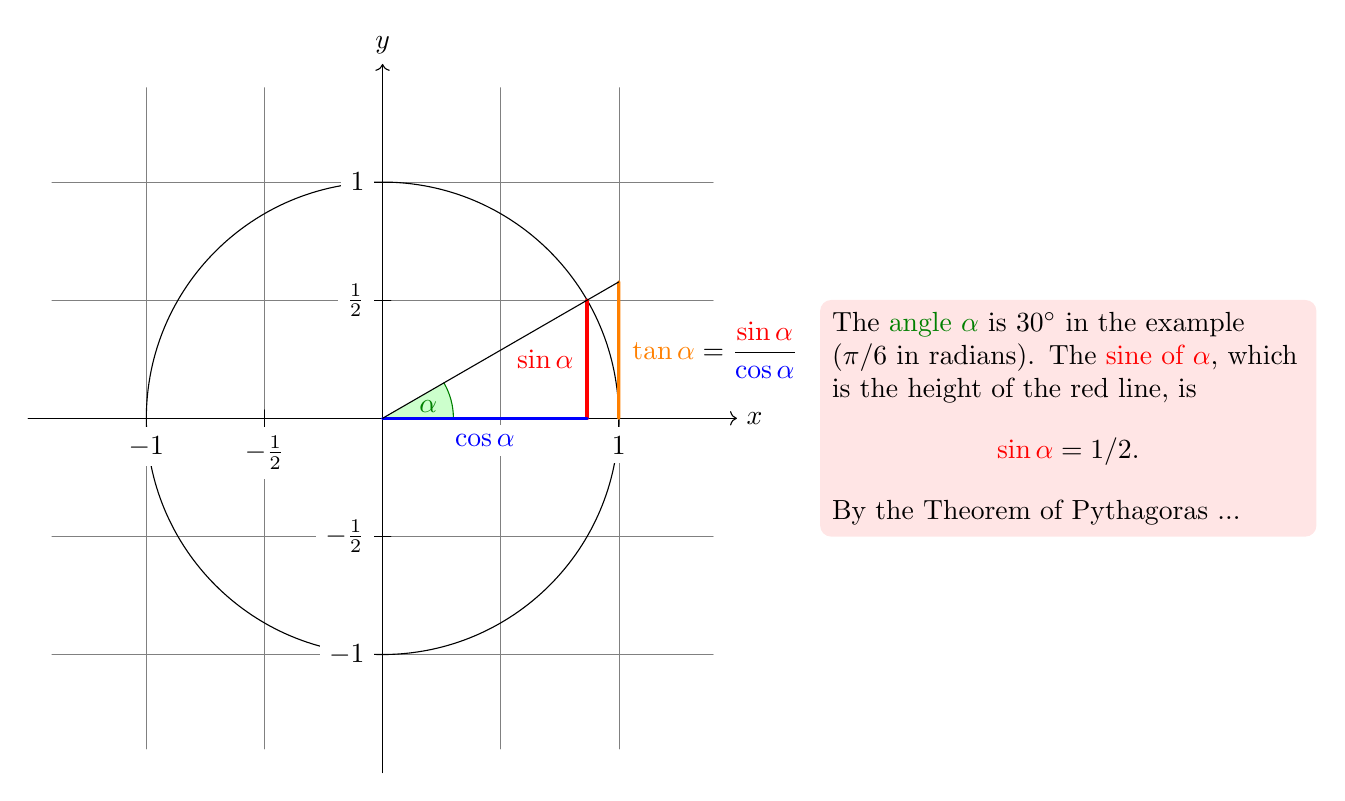
\begin{tikzpicture}
[scale=3,line cap=round,axes/.style=,important line/.style={very thick},
information text/.style={rounded corners,fill=red!10,inner sep=1ex}]
% Colors
\colorlet{anglecolor}{green!50!black}
\colorlet{sincolor}{red}
\colorlet{tancolor}{orange!80!black}
\colorlet{coscolor}{blue}
% The graphic
\draw[help lines,step=0.5cm] (-1.4,-1.4) grid (1.4,1.4);
\draw (0,0) circle [radius=1cm];
\begin{scope}
\draw[->] (-1.5,0) -- (1.5,0) node[right] {$x$} coordinate(x axis);
\draw[->] (0,-1.5) -- (0,1.5) node[above] {$y$} coordinate(y axis);
\foreach \x/\xtext in {-1, -.5/-\frac{1}{2}, 1}
\draw[xshift=\x cm] (0pt,1pt) -- (0pt,-1pt) node[below,fill=white] {$\xtext$};
\foreach \y/\ytext in {-1, -.5/-\frac{1}{2}, .5/\frac{1}{2}, 1}
\draw[yshift=\y cm] (1pt,0pt) -- (-1pt,0pt) node[left,fill=white] {$\ytext$};
\end{scope}
\filldraw[fill=green!20,draw=anglecolor] (0,0) -- (3mm,0pt)
arc [start angle=0, end angle=30, radius=3mm];
\draw (15:2mm) node[anglecolor] {$\alpha$};
\draw[important line,sincolor]
(30:1cm) -- node[left=1pt,fill=white] {$\sin \alpha$} (30:1cm |- x axis);
\draw[important line,coscolor]
(30:1cm |- x axis) -- node[below=2pt,fill=white] {$\cos \alpha$} (0,0);
\path [name path=upward line] (1,0) -- (1,1);
\path [name path=sloped line] (0,0) -- (30:1.5cm);
\draw [name intersections={of=upward line and sloped line, by=t}]
[very thick,orange] (1,0) -- node [right=1pt,fill=white]
{$\displaystyle \tan \alpha \color{black}=
\frac{{\color{red}\sin \alpha}}{\color{blue}\cos \alpha}$} (t);
\draw (0,0) -- (t);
\draw[xshift=1.85cm]
node[right,text width=6cm,information text]
{
The {\color{anglecolor} angle $\alpha$} is $30^\circ$ in the
example ($\pi/6$ in radians). The {\color{sincolor}sine of
$\alpha$}, which is the height of the red line, is
\[
{\color{sincolor} \sin \alpha} = 1/2.
\]
By the Theorem of Pythagoras ...
};
\end{tikzpicture}
\end{figure}

\begin{lstlisting}[name=example-1,numbers=left,    numberstyle=\footnotesize]
\begin{tikzpicture}
[scale=3,line cap=round,
% Styles
axes/.style=,
important line/.style={very thick},
information text/.style={rounded corners,
                              fill=red!10,inner sep=1ex}]
% Colors
\colorlet{anglecolor}{green!50!black}
\colorlet{sincolor}{red}
\colorlet{tancolor}{orange!80!black}
\colorlet{coscolor}{blue}
\end{lstlisting}

1行,开启tikzpicture环境。

2行,scale=3,缩放比例为3。line cap=round,线的端头采用圆形(rect为方形,butt为无头)。

4行,axes 采用默认样式。

5行,定义important line的样式,只要求线宽为very thick。

6行,定义information text的样式,圆角边框,颜色为red!10,文字与文字背景边界距离为1ex。

9行,命令 \verb!\colorlet! 定义颜色green!50!black的名称为anglecolor,可以用此名称引用该颜色。10、11、12行类似。

\begin{lstlisting}[name=example-1,numbers=left,    numberstyle=\footnotesize]
% The graphic
\draw[help lines,step=0.5cm] (-1.4,-1.4) grid (1.4,1.4);
\draw (0,0) circle [radius=1cm];
\begin{scope}[axes]
\draw[->] (-1.5,0) -- (1.5,0) node[right] {$x$} 
            coordinate(x axis);
\draw[->] (0,-1.5) -- (0,1.5) node[above] {$y$} 
            coordinate(y axis);
\foreach \x/\xtext in {-1, -.5/-\frac{1}{2}, 1}
\draw[xshift=\x cm] (0pt,1pt) -- (0pt,-1pt) 
                     node[below,fill=white] {$\xtext$};
\foreach \y/\ytext in {-1, -.5/-\frac{1}{2}, .5/\frac{1}{2}, 1}
\draw[yshift=\y cm] (1pt,0pt) -- (-1pt,0pt) 
                     node[left,fill=white] {$\ytext$};
\end{scope}
\end{lstlisting}

14行,\verb!\draw!命令开始绘图,grid 是网格命令,采用help lines的样式,步长step=0.5cm,以点(-1.4,-1.4)到(1.4,1.4)为对角线。

15行,画圆,圆心为(0,0),半径为radius=1cm。

16行,开启scope环境,即在整个大图中再绘制一个局部图。

17行,从(-1.5,0)到(1.5,0)画线段,选项[->]为线段末端添加箭头;点(1.5,0)后的node命令为该点添加标签,选项[right]指示标签在点的右侧,标签是 \LaTeX 符号$x$。

21行,\verb!\foreach!命令指示对数组中的每个元素进行后面的操作。\verb!\x/\xtext!
表示数组元素可以是\verb!\x!形式的或\verb!\x/\xtext!形式的;同一个元素位置上用符号/并列两种形式时,该元素可用两种形式之一引用。数组 \{1,...,10\}是公差为1的等差数列,数组\{1,1.5,,...,10\}是公差为前两项之差0.5的等差数列。

22行,是21行的\verb!\foreach!命令指向的操作。选项 \verb![xshift=\x cm]!指示将后面绘制的线段沿着x轴平移 \verb!\x cm!。

23行,node命令为22行的点(0pt,-1pt)加标签,标签用 \verb!$\xtext$!形式。选项[below,fill=white]表示标签在点下方,标签背景为白色。

27行,结束scope环境。

\begin{lstlisting}[name=example-1,numbers=left,    numberstyle=\footnotesize]
\filldraw[fill=green!20,draw=anglecolor] (0,0) -- (3mm,0pt)
arc [start angle=0, end angle=30, radius=3mm];
\draw (15:2mm) node[anglecolor] {$\alpha$};
\draw[important line,sincolor]
      (30:1cm) -- node[left=1pt,fill=white] {$\sin \alpha$} 
      (30:1cm |- x axis);
\draw[important line,coscolor]
      (30:1cm |- x axis) -- node[below=2pt,fill=white] 
      {$\cos \alpha$} (0,0);
\path [name path=upward line] (1,0) -- (1,1);
\path [name path=sloped line] (0,0) -- (30:1.5cm);
\draw [name intersections={of=upward line and sloped line, by=t}]
      [very thick,orange] (1,0) -- node [right=1pt,fill=white]
{$\displaystyle \tan \alpha \color{black}=
\frac{{\color{red}\sin \alpha}}{\color{blue}\cos \alpha}$}(t);
\draw (0,0) -- (t);
\end{lstlisting}

28行,\verb!\filldraw!是填充颜色命令\verb!\fill!和绘图命令\verb!\draw!的结合。fill=green!20表示用颜色green!20填充,draw=anglecolor表示用颜色anglecolor(已在9行定义)绘图。

29行,arc命令绘制圆弧线,选项start angle=0表示起始角度是$0^{\circ}$,end angle=30表示终止角度是$30^{\circ}$,radius=3mm表示半径是3mm,默认圆心是(0,0)。

30行,极坐标点(15:2mm)是$15^{\circ}$,2mm的点。

31行,选项important line,sincolor已在5行,10行定义。

32行,node命令在连接符号\verb!--!之后,表示标签加在路径中间,标签 \verb!$\sin \alpha$!是 \LaTeX 符号$\sin \alpha$。

33行,表示过点(30:1cm)的竖直线与x轴的交点。

35行,node命令的选项below=2pt表示标签在路径下方2pt处,fill=white表示标签文字背景填充为白色。

37行,\verb!\path!命令声明它后面的对象是路径,这里的路径是个线段,选项name path=upward line即命名路径为upward line。

39行,选项表示命名交点,把路径upward line与sloped line的交点记命名为t。

41行,\LaTeX 命令 \verb!\displaystyle!定义显示公式样式,注意颜色命令 \verb!\color{black}!只对42行的分数线有作用。


\begin{lstlisting}[name=example-1,numbers=left,    numberstyle=\footnotesize]
\draw[xshift=1.85cm]
       node[right,text width=6cm,information text]
{
  The {\color{anglecolor} angle $\alpha$} is $30^\circ$ in the
  example ($\pi/6$ in radians). The {\color{sincolor}sine of
  $\alpha$}, which is the height of the red line, is
  \[
    {\color{sincolor} \sin \alpha} = 1/2.
  \]
  By the Theorem of Pythagoras ...
};
\end{tikzpicture}
\end{lstlisting}

44行,选项[xshift=1.85cm]将绘制的标签右移1.85cm。

45行至54行,给原点加的标签,按44行的选项平移。

55行,结束\{tikzpicture\}环境。




\subsection{A Petri-Net}

本小节展示的代码绘制下面的图形
\begin{figure}[h]
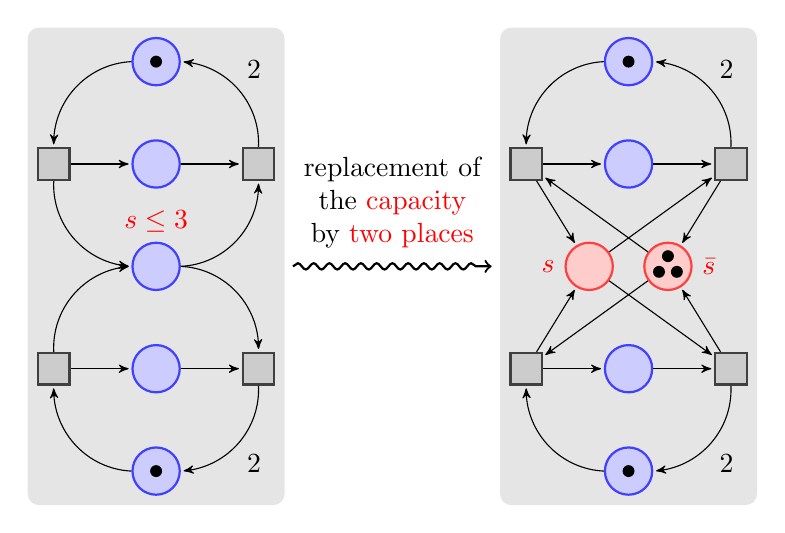
\begin{tikzpicture}
[node distance=1.3cm,on grid,>=stealth',bend angle=45,auto,
 every place/.style= {minimum size=6mm,thick,draw=blue!75,fill=blue!20},
 every transition/.style={thick,draw=black!75,fill=black!20},
red place/.style= {place,draw=red!75,fill=red!20},
every label/.style= {red}]

\node [place,tokens=1] (w1) {};
\node [place] (c1) [below=of w1] {};
\node [place] (s) [below=of c1,label=above:$s\le 3$] {};
\node [place] (c2) [below=of s] {};
\node [place,tokens=1] (w2) [below=of c2] {};
\node [transition] (e1) [left=of c1] {}
edge [pre,bend left] (w1)
edge [post,bend right] (s)
edge [post] (c1);
\node [transition] (e2) [left=of c2] {}
edge [pre,bend right] (w2)
edge [post,bend left] (s)
edge [post] (c2);
\node [transition] (l1) [right=of c1] {}
edge [pre] (c1)
edge [pre,bend left] (s)
edge [post,bend right] node[swap] {2} (w1);
\node [transition] (l2) [right=of c2] {}
edge [pre] (c2)
edge [pre,bend right] (s)
edge [post,bend left] node {2} (w2);

\begin{scope}[xshift=6cm]
\node [place,tokens=1] (w1’) {};
\node [place] (c1’) [below=of w1’] {};
\node [red place] (s1’) [below=of c1’,xshift=-5mm]
[label=left:$s$] {};
\node [red place,tokens=3] (s2’) [below=of c1’,xshift=5mm]
[label=right:$\bar s$] {};
\node [place] (c2’) [below=of s1’,xshift=5mm] {};
\node [place,tokens=1] (w2’) [below=of c2’] {};
\node [transition] (e1’) [left=of c1’] {}
edge [pre,bend left] (w1’)
edge [post] (s1’)
edge [pre] (s2’)
edge [post] (c1’);
\node [transition] (e2’) [left=of c2’] {}
edge [pre,bend right] (w2’)
edge [post] (s1’)
edge [pre] (s2’)
edge [post] (c2’);
\node [transition] (l1’) [right=of c1’] {}
edge [pre] (c1’)
edge [pre] (s1’)
edge [post] (s2’)
edge [post,bend right] node[swap] {2} (w1’);
\node [transition] (l2’) [right=of c2’] {}
edge [pre] (c2’)
edge [pre] (s1’)
edge [post] (s2’)
edge [post,bend left] node {2} (w2’);
\end{scope}

\begin{scope}[on background layer]
\node (r1) [fill=black!10,rounded corners,fit=(w1)(w2)(e1)(e2)(l1)(l2)] {};
\node (r2) [fill=black!10,rounded corners,fit=(w1’)(w2’)(e1’)(e2’)(l1’)(l2’)] {};
\end{scope}
\draw [shorten >=1mm,-to,thick,decorate,
decoration={snake,amplitude=.4mm,segment length=2mm,
pre=moveto,pre length=1mm,post length=2mm}]
(r1) -- (r2) node [above=1mm,midway,text width=3cm,align=center]
{replacement of the \textcolor{red}{capacity} by \textcolor{red}{two places}};
\end{tikzpicture}
\end{figure}

\begin{lstlisting}[name=example-2,numbers=left,    numberstyle=\footnotesize]
\begin{tikzpicture}
      [node distance=1.3cm,on grid,>=stealth',bend angle=45,auto,
       every place/.style= {minimum size=6mm,thick,draw=blue!75,fill=blue!20},
       every transition/.style={thick,draw=black!75,fill=black!20},
       red place/.style= {place,draw=red!75,fill=red!20},
       every label/.style= {red}]
\end{lstlisting}

2行,\verb!node distance!确定node的间距,如下设置该间距 \\
\verb!node distance=距离! \\
当环境带有on grid选项时,该值指的是node的中心之间的距离;当环境无on grid选项时,该值指的是node边界之间的距离,初始值为1cm。>=stealth’指示箭头样式。bend angle=45指示路径的转弯角度。auto指示路径标签与路径的相对位置。用 \\
\verb!auto=direction! \\
设置auto的位置,其中direction可以是left,right,false;当为路径标签选择above,below等位置时,或使用anchor选项时,auto的值是false;auto的值默认是scope的设置。

3行,every place定义所有place的样式。minimum size=6mm是最小尺寸为6mm;draw=blue!75,用颜色blue!75画出边界线;fill=blue!20,用颜色blue!20填充标签。

5行,定义 red place样式,其中调用了place样式。

6行,every label定义所有lable的样式。

\begin{lstlisting}[name=example-2,numbers=left,    numberstyle=\footnotesize]
\node [place,tokens=1] (w1)  {};
\node [place] (c1) [below=of w1] {};
\node [place] (s) [below=of c1,label=above:$s\le 3$] {};
\node [place] (c2) [below=of s] {};
\node [place,tokens=1] (w2) [below=of c2] {};
\node [transition] (e1) [left=of c1] {}
                        edge [pre,bend left] (w1)
                        edge [post,bend right] (s)
                        edge [post] (c1);
\node [transition] (e2) [left=of c2] {}
                        edge [pre,bend right] (w2)
                        edge [post,bend left] (s)
                        edge [post] (c2);
\node [transition] (l1) [right=of c1] {}
                        edge [pre] (c1)
                        edge [pre,bend left] (s)
                        edge [post,bend right] node[swap] {2} (w1);
\node [transition] (l2) [right=of c2] {}
                        edge [pre] (c2)
                        edge [pre,bend right] (s)
                        edge [post,bend left] node {2} (w2);
\end{lstlisting}

7行,命令 \verb!\node!指示绘制标签。选项place已在3行定义。tokens=1指示标记数目为1,(w1)中的w1是标签的名称。花括号无内容,表示标签无文字(但不能省略花括号)。

8行,(c1)指示标签的名称为c1。选项below=of w1表示标签在7行定义的标签w1的下方。

9行,选项 \verb!label=above:$s\le 3$!指示在node的上面加 \LaTeX 标签$s\le 3$。

12行,选项transition已在4行定义。

13-15行,从12行的e1分别向w1,s,c1画线,注意13、14行无分号,15行有分号。(选项pre,post)。bend left=angle,以出发点为原点,起点至终点的位移方向为初始边方向,逆时针方向为正,这样规定下的angle是起点处的出发方向;负的angle是终点处的进入方向。bend right=angle的意思与之类似,只是角的方向相反。如果不指定角度,它的默认值是前面最近出现的角度。

17-19行,从16行的e2向w2,s,c2画线。注意17、18行无分号,19行有分号。

23行,node给该行的edge加标签,标签内容是2。选项swap指示标签的位置与2行的auto规定的位置相反。

27行,node给该行的edge加标签。标签内容是2。

\begin{lstlisting}[name=example-2,numbers=left,    numberstyle=\footnotesize]
\begin{scope}[xshift=6cm]
\node [place,tokens=1] (w1’) {};
\node [place] (c1’) [below=of w1’] {};
\node [red place] (s1’) [below=of c1’,xshift=-5mm]
      [label=left:$s$] {};
\node [red place,tokens=3] (s2’) [below=of c1’,xshift=5mm]
      [label=right:$\bar s$] {};
\node [place] (c2’) [below=of s1’,xshift=5mm] {};
\node [place,tokens=1] (w2’) [below=of c2’] {};
\node [transition] (e1’) [left=of c1’] {}
                         edge [pre,bend left] (w1’)
                         edge [post] (s1’)
                         edge [pre] (s2’)
                         edge [post] (c1’);
\node [transition] (e2’) [left=of c2’] {}
                         edge [pre,bend right] (w2’)
                         edge [post] (s1’)
                         edge [pre] (s2’)
                         edge [post] (c2’);
\node [transition] (l1’) [right=of c1’] {}
                         edge [pre] (c1’)
                         edge [pre] (s1’)
                         edge [post] (s2’)
                         edge [post,bend right] node[swap] {2} (w1’);
\node [transition] (l2’) [right=of c2’] {}
                         edge [pre] (c2’)
                         edge [pre] (s1’)
                         edge [post] (s2’)
                         edge [post,bend left] node {2} (w2’);
\end{scope}
\end{lstlisting}

28行,开启scope环境,选项xshift=6cm使得环境生成的图右移6cm。

31行,选项xshift=-5mm使得标签左移5mm。

32行,给node加标签,选项left指示标签在node的左侧。

56行,node给edge加标签,标签内容是2。标签位置参照2行auto的指示。

57行,结束scope环境。

\begin{lstlisting}[name=example-2,numbers=left,    numberstyle=\footnotesize]
\begin{scope}[on background layer]
\node (r1) [fill=black!10,rounded corners,
             fit=(w1)(w2)(e1)(e2)(l1)(l2)] {};
\node (r2) [fill=black!10,rounded corners,
             fit=(w1’)(w2’)(e1’)(e2’)(l1’)(l2’)] {};
\end{scope}
\draw [shorten >=1mm,-to,thick,decorate,
       decoration={snake,amplitude=.4mm,segment length=2mm,
       pre=moveto,pre length=1mm,post length=2mm}]
      (r1) -- (r2) node [above=1mm,midway,
                          text width=3cm,align=center]
                         {replacement of the \textcolor{red}{capacity} 
                          by \textcolor{red}{two places}};
\end{tikzpicture}
\end{lstlisting}

58行,选项on background layer指示开启的scope环境所在的层属于主层(即tikzpicture环境所在层)之下的层。

59行,选项rounded corners指示标签边框用圆角。

60行,选项fit生成一个盒子(fit=(w1)(w2)(e1)(e2)(l1)(l2),等号右侧各项是坐标或node,各项之间不能加逗号),生成的盒子将等号右侧各项包围在内。各项与盒子边界的距离用选项inner sep=设置。



\subsection{平面几何绘图举例}

\subsubsection{Elements' Book I, Proposition I}

本小节展示的代码绘制下面的图形
\begin{figure}[h]
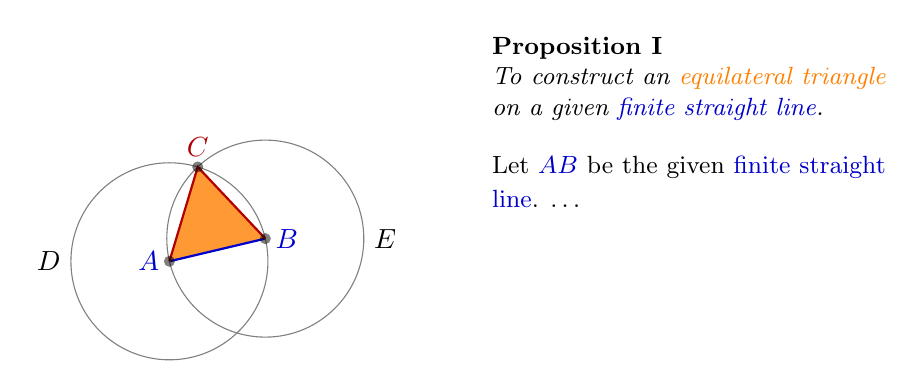
\begin{tikzpicture}[thick,help lines/.style={thin,draw=black!50}]
\def\A{\textcolor{input}{$A$}} \def\B{\textcolor{input}{$B$}}
\def\C{\textcolor{output}{$C$}} \def\D{$D$}
\def\E{$E$}
\colorlet{input}{blue!80!black} \colorlet{output}{red!70!black}
\colorlet{triangle}{orange}
\coordinate [label=left:\A] (A) at ($ (0,0) + .1*(rand,rand) $);
\coordinate [label=right:\B] (B) at ($ (1.25,0.25) + .1*(rand,rand) $);
\draw [input] (A) -- (B);
\node [name path=D,help lines,draw,label=left:\D] (D) at (A) [circle through=(B)] {};
\node [name path=E,help lines,draw,label=right:\E] (E) at (B) [circle through=(A)] {};
\path [name intersections={of=D and E,by={[label=above:\C]C}}];
\draw [output] (A) -- (C) -- (B);
\foreach \point in {A,B,C}
\fill [black,opacity=.5] (\point) circle (2pt);
\begin{pgfonlayer}{background}
\fill[triangle!80] (A) -- (C) -- (B) -- cycle;
\end{pgfonlayer}
\node [below right, text width=5cm,align=justify] at (4,3) {
\small\textbf{Proposition I}\par
\emph{To construct an \textcolor{triangle}{equilateral triangle}
on a given \textcolor{input}{finite straight line}.}
\par\vskip1em
Let \A\B\ be the given \textcolor{input}{finite straight line}. \dots
};
\end{tikzpicture}
\end{figure}

\begin{lstlisting}[name=example-3.1,numbers=left,    numberstyle=\footnotesize]
\begin{tikzpicture}[thick,help lines/.style={thin,draw=black!50}]
\def\A{\textcolor{input}{$A$}} 
\def\B{\textcolor{input}{$B$}}
\def\C{\textcolor{output}{$C$}} 
\def\D{$D$}
\def\E{$E$}
\colorlet{input}{blue!80!black} 
\colorlet{output}{red!70!black}
\colorlet{triangle}{orange}
\end{lstlisting}

1行,选项thick定义环境中的路径的线宽,help lines/.style=定义help lines的样式。

2行,\verb!\def!开启定义功能,\verb!\A!是定义的名称,\verb!{\textcolor{input}{$A$}}!是\verb!\A!的内容。

7行,\verb!\colorlet!开启定义颜色功能,\verb!{input}!是颜色名称,\verb.{blue!80!black}.是定义的颜色。

\begin{lstlisting}[name=example-3.1,numbers=left,    numberstyle=\footnotesize]
\coordinate [label=left:\A] (A) 
             at ($ (0,0) + .1*(rand,rand) $);
\coordinate [label=right:\B] (B) 
             at ($ (1.25,0.25) + .1*(rand,rand) $);
\draw [input] (A) -- (B);
\node [name path=D,help lines,draw,label=left:\D] (D) 
       at (A) [circle through=(B)] {};
\node [name path=E,help lines,draw,label=right:\E] (E) 
       at (B) [circle through=(A)] {};
\path [name intersections={of=D and E,by={[label=above:\C]C}}];
\draw [output] (A) -- (C) -- (B);
\foreach \point in {A,B,C}
\fill [black,opacity=.5] (\point) circle (2pt);
\end{lstlisting}

10行,\verb!\coordinate!开启定义坐标功能,选项 \verb!label=left:\A!指示给坐标加标签,标签在坐标的left侧,标签内容是2行定义的“\verb!\A!”;括号(A) 是定义的坐标的名称,at指示坐标的位置;\verb!($ (0,0) + .1*(rand,rand) $)!用向量运算定义一个点,其中rand是-1到1之间的随机数,注意分数或小数与rand相乘必须加*符号,两个美元符号表示计算,而不是 \LaTeX 的数学模式。

14行,画线段AB。

15行,\verb!\node!开启node(加标签)功能;选项name path=D定义node的边界是名称为D的路径;选项help lines调用1行定义的help lines样式;选项draw指示画出边界路径;括号(D)是该node的名称。

16行,at指示15行的node所指向的对象位置;(A)是node所指向的对象;(A) [circle through=(B)]画以(A) 为圆心,经过点(B)的圆,需要调用through程序库;花括号\{\}内是node的内容,尽管无内容,但不能没有花括号。

19行,\verb!\path!开启定义路径功能;\verb!name intersections=!用来定义两个路径的交点;of=D and E指示分析路径D和E的交点;\verb!by=!指示用C来做交点名称,而C带有标签\verb!{[label=above:\C]C}!,注意必须用花括号把\verb![label=above:\C]C!括起来。

21行,\verb!\foreach!开启foreach操作模式,对数组\verb!{A,B,C}!内的每个元素(用\verb!\point!代表)进行相同的操作。

22行,即21行\verb!\foreach!指向的操作。\verb!\fill!指示填充颜色;选项opacity=.5设置不透明度为0.5;circle命令指示以 \verb!\point!为圆心,以2pt为半径画圆;\verb!\fill!以半透明的黑色填充该圆,实际上是描三点A,B,C。

\begin{lstlisting}[name=example-3.1,numbers=left,    numberstyle=\footnotesize]
\begin{pgfonlayer}{background}
\fill[triangle!80] (A) -- (C) -- (B) -- cycle;
\end{pgfonlayer}
\node [below right, text width=5cm,align=justify] at (4,3) 
      {\small\textbf{Proposition I} \par 
           \emph{To construct an 
                 \textcolor{triangle}{equilateral triangle}
                 on a given 
                 \textcolor{input}{finite straight line}.}
           \par\vskip1em
        Let \A\B\ be the given 
        \textcolor{input}{finite straight line}. \dots
       };
\end{tikzpicture}
\end{lstlisting}

23行,在background层上作图。

25行,结束background层上作图。

26行,给(4,3) 点加标签,内容是一段文字。below right指示标签在点(4,3)的右下方;text width=5cm设置每行文字宽度为10cm;align=justify设置文字对齐方式是自适应方式。


\subsubsection{Elements' Book I, Proposition II}

本小节展示的代码绘制下面的图形
\begin{figure}[h]
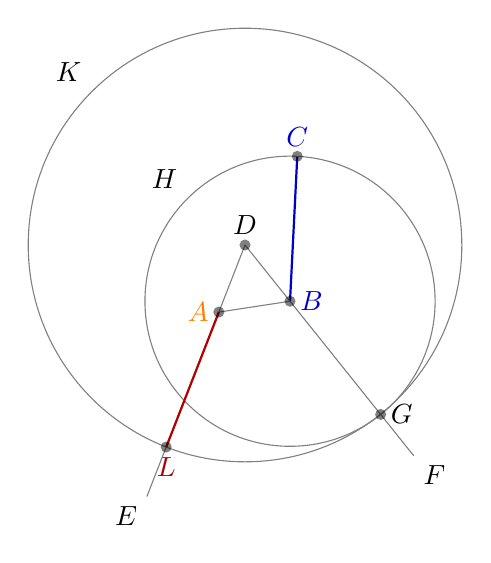
\begin{tikzpicture}[thick,help lines/.style={thin,draw=black!50}]
\def\A{\textcolor{orange}{$A$}} \def\B{\textcolor{input}{$B$}}
\def\C{\textcolor{input}{$C$}} \def\D{$D$}
\def\E{$E$} \def\F{$F$}
\def\G{$G$} \def\H{$H$}
\def\K{$K$} \def\L{\textcolor{output}{$L$}}
\colorlet{input}{blue!80!black} \colorlet{output}{red!70!black}
\coordinate [label=left:\A] (A) at ($ (0,0) + .1*(rand,rand) $);
\coordinate [label=right:\B] (B) at ($ (1,0.2) + .1*(rand,rand) $);
\coordinate [label=above:\C] (C) at ($ (1,2) + .1*(rand,rand) $);
\draw [input] (B) -- (C);
\draw [help lines] (A) -- (B);
\coordinate [label=above:\D] (D) at ($ (A)!.5!(B) ! {sin(60)*2} ! 90:(B) $);
\draw [help lines] (D) -- ($ (D)!3.75!(A) $) coordinate [label=-135:\E] (E);
\draw [help lines] (D) -- ($ (D)!3.75!(B) $) coordinate [label=-45:\F] (F);
\node (H) at (B) [name path=H,help lines,circle through=(C),draw,label=135:\H] {};
\path [name path=B--F] (B) -- (F);
\path [name intersections={of=H and B--F,by={[label=right:\G]G}}];
\node (K) at (D) [name path=K,help lines,circle through=(G),draw,label=135:\K] {};
\path [name path=A--E] (A) -- (E);
\path [name intersections={of=K and A--E,by={[label=below:\L]L}}];
\draw [output] (A) -- (L);
\foreach \point in {A,B,C,D,G,L}
\fill [black,opacity=.5] (\point) circle (2pt);
\end{tikzpicture}
\end{figure}

\begin{lstlisting}[name=example-3.2,numbers=left,    numberstyle=\footnotesize]
\begin{tikzpicture}[thick,help lines/.style={thin,draw=black!50}]
\def\A{\textcolor{orange}{$A$}} 
\def\B{\textcolor{input}{$B$}}
\def\C{\textcolor{input}{$C$}} 
\def\D{$D$}
\def\E{$E$} 
\def\F{$F$}
\def\G{$G$} 
\def\H{$H$}
\def\K{$K$} 
\def\L{\textcolor{output}{$L$}}
\colorlet{input}{blue!80!black} 
\colorlet{output}{red!70!black}
\coordinate [label=left:\A] (A) 
              at ($ (0,0) + .1*(rand,rand) $);
\coordinate [label=right:\B] (B) 
              at ($ (1,0.2) + .1*(rand,rand) $);
\coordinate [label=above:\C] (C) 
              at ($ (1,2) + .1*(rand,rand) $);
\end{lstlisting}

以上主要是为后面画图作定义。

\begin{lstlisting}[name=example-3.2,numbers=left,    numberstyle=\footnotesize]
\draw [input] (B) -- (C);
\draw [help lines] (A) -- (B);
\coordinate [label=above:\D] (D) 
      at ($ (A)!.5!(B) ! {sin(60)*2} ! 90:(B) $);
\draw [help lines] (D) -- ($ (D)!3.75!(A) $) 
         coordinate [label=-135:\E] (E);
\draw [help lines] (D) -- ($ (D)!3.75!(B) $) 
         coordinate [label=-45:\F] (F);
\node (H) at (B) 
      [name path=H,help lines,circle through=(C),
         draw,label=135:\H] {};
\path [name path=B--F] (B) -- (F);
\path [name intersections={of=H and B--F,
                            by={[label=right:\G]G}}];
\node (K) at (D) 
      [name path=K,help lines,circle through=(G),
         draw,label=135:\K] {};
\path [name path=A--E] (A) -- (E);
\path [name intersections={of=K and A--E,
                            by={[label=below:\L]L}}];
\draw [output] (A) -- (L);
\foreach \point in {A,B,C,D,G,L}
\fill [black,opacity=.5] (\point) circle (2pt);
\end{tikzpicture}
\end{lstlisting}

23行,表达式\verb.($ (A)!x!(B) $).确定直线AB上一个点,如果x在0到1之间,该点在线段AB内部;如果x大于1,该点在AB外部;如果x是正数,则该点与A、B的距离之比为x;如果x是负数,则该点是点\verb.($ (A)!|x|!(B) $).关于点A的对称点。

表达式\verb.($ (X) ! {sin(60)*2} ! 90:(B) $).指示以X为基点,将线段XB绕X旋转90度,再伸长sin(60)*2倍后,得到的线段端点。


表达式\verb&($ (A) ! .5 ! (B) ! {sin(60)*2} ! 90:(B) $)&指示先运算
\verb&($ (A)!.5!(B) $)&得到一个点,然后该点参与后面的运算。


\section{Tikz 的绘图环境和命令}

在 \LaTeX 中,要用 tikz 作图,首先调用 tikz 宏包和有关的程序库
\begin{lstlisting}
\usepackage{tikz}
\usetikzlibrary{<list of libraries>}
\end{lstlisting}
然后开启\{tikzpicture\}环境作图,或者用命令 \verb=\tikz=开始作图。

{\large \heiti \color{red} 各种命令必须以分号结束,否则报错。 }



\subsection{\{tikzpicture\}环境或 tikz 命令的格式}

\begin{lstlisting}
环境格式
\begin{tikzpicture}[<options>]
<environment contents>
\end{tikzpicture}

命令格式
\tikz[<options>]{<path commands>}
例如,\tikz{\draw (0,0) rectangle (2ex,1ex);}
\end{lstlisting}



\subsection{主要的绘图对象}

绘图时涉及的主要对象有
\begin{itemize}
\item 点

符号 (1,2) 指定笛卡尔坐标点,默认坐标单位长度是 1cm。

符号\verb=(30:1cm)=指定极坐标点,其中30表示 $30^{\circ}$。

符号\verb=(30:1cm |- 0,0)=表示过点\verb=(30:1cm)=的竖直线与过\verb=(0cm,0cm)=点的水平线的交点。(2,1 |- 3,4) 与 (3,4 -| 2,1) 所定义的点相同。注意其中坐标没有括号。

\item 线

主要有直线和曲线。

\item Path

以命令 \verb!\path! 开头的句子创建一个 path 对象,构成路径的元素可以是点,线,node,图形等,不仅仅只有点和线。

\item Coordinate

以命令 \verb!\coordinate! 开头的句子将某个对象(可以是点,线,node,图形等)设置为 coordinate 对象。注意点与 coordinate 对象不同,coordinate 对象可以带多个选项使得其本身的内容更加丰富,而点则不能。

\item Node

以命令 \verb!\node! 开头的句子将某个对象(可以是点,线,node,图形等)设置为 node 对象,可以为 node 对象设置位置,边界形状,文字,颜色,标签等属性。
\end{itemize}

注意,创建了以上对象不等于显示它们,要显示创建的对象需要给这些命令添加选项 draw,或者用 \verb!\draw! 开头的语句来绘图。

\verb!\draw <path>;! 相当于 \verb!\path [draw] ...;!。



\subsection{命令 \textbackslash def}

命令 \verb=\def= 用于自定义一个对象,该对象名称以反斜线 \textbackslash 开头。句法是
\begin{lstlisting}
\def<对象名称>{定义内容};
\end{lstlisting}

下面的例子定义 \verb!\wall! (需要调用 pattern 程序库)\\
{\begin{minipage}{12cm}
\begin{lstlisting}
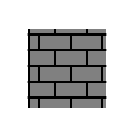
\begin{tikzpicture}
\def\wall{ \fill [fill=black!50] (1,-.5) rectangle (2,.5);
          \pattern [pattern=bricks] (1,-.5) rectangle (2,.5);
          \draw [line width=1pt] (1cm+.5pt,-.5) -- ++(0,1); }
\wall
\end{tikzpicture}
\end{lstlisting}
\end{minipage}
\hspace{1cm}
{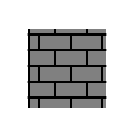
\begin{tikzpicture}
\def\wall{ \fill [fill=black!50] (1,-.5) rectangle (2,.5);
\pattern [pattern=bricks] (1,-.5) rectangle (2,.5);
\draw [line width=1pt] (1cm+.5pt,-.5) -- ++(0,1); }
\wall
\end{tikzpicture}}}


\subsection{创建 coordinate 对象的句法及其命名}

创建 coordinate 对象的句法是
\begin{lstlisting}
\path . . . coordinate[<options>](<name>)at(<coordinate>) . . . ;
将路径中的某个对象设置为 coordinate 对象,这个对象可以是点,线,node,标签等等。
\end{lstlisting}

\begin{lstlisting}
\coordinate  [<options>](<name>)at(<coordinate>);
这是上一句法的简写,注意最好不要在该命令后面用 node 命令。
\end{lstlisting}



\subsection{Bounding Box}

盒子是一个占据一定空间的对象,盒子有宽度(width),基线(baseline),基线到盒子的上界是高度(height),基线到盒子下界是深度(depth)。默认基线是图形的 x 轴。

将绘制的图形作为盒子,可用如下的选项或命令
\begin{lstlisting}
选项 use as bounding box
命令 \useasboundingbox,是 \path[use as bounding box] 的简写。
\end{lstlisting}

\noindent{\begin{minipage}{8cm}
\begin{lstlisting}
Left of picture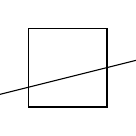
\begin{tikzpicture}
\draw[use as bounding box] 
      (2,0) rectangle (3,1);
\draw (1,0) -- (4,.75);
\end{tikzpicture}right of picture.
\end{lstlisting}
\end{minipage} 
\hspace{1cm}
Left of picture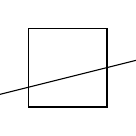
\begin{tikzpicture}
\draw[use as bounding box] (2,0) rectangle (3,1);
\draw (1,0) -- (4,.75);
\end{tikzpicture}right of picture. 
}

\noindent{\begin{minipage}{8cm}
\begin{lstlisting}
Left of picture

\begin{tikzpicture}
\useasboundingbox (0,0) rectangle (3,1);
\fill (.75,.25) circle (.5cm);
\end{tikzpicture}
right of picture.
\end{lstlisting}
\end{minipage} 
\hspace{0.1cm}
Left of picture

\begin{tikzpicture}
\useasboundingbox (0,0) rectangle (3,1);
\fill (.75,.25) circle (.5cm);
\end{tikzpicture}
right of picture.
}

\begin{lstlisting}
选项current bounding box
选项current path bounding box
这两个选项可以把当前的图形或者路径看作矩形盒子。
\end{lstlisting}

\begin{lstlisting}
trim left=<dimension or coordinate or default> 该选项将图形向左平移,将位置 x=dimension 
作为当前盒子的边界,该位置左侧的部分会被盒子左侧的内容覆盖,默认 0pt(即(0,0))。
trim left=<dimension or coordinate> 意义类似,只是没有默认值。
\end{lstlisting}

\begin{lstlisting}
Text before image.
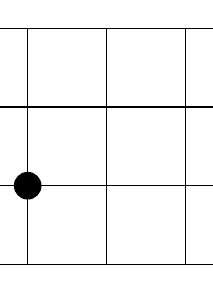
\begin{tikzpicture}[trim left, trim right=2cm, baseline]
\draw (-1,-1) grid (3,2);
\fill (0,0) circle (5pt);
\end{tikzpicture}
\end{lstlisting}
Text before image.
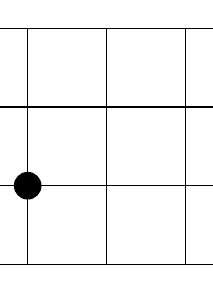
\begin{tikzpicture}[trim left, trim right=2cm, baseline]
\draw (-1,-1) grid (3,2);
\fill (0,0) circle (5pt);
\end{tikzpicture}
Text after image.

\noindent{\begin{minipage}{8cm}
\begin{lstlisting}
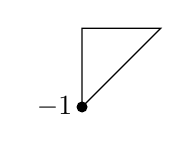
\begin{tikzpicture}
\draw (0,1) -- (0,0) -- (1,1) -- cycle;
\fill (0,0) circle (2pt);
\node[left] at (0,0) {$-1$};
\end{tikzpicture}
\par
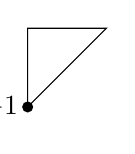
\begin{tikzpicture}[trim left]
\draw (0,1) -- (0,0) -- (1,1) -- cycle;
\fill (0,0) circle (2pt);
\node[left] at (0,0) {$-1$};
\end{tikzpicture}
\end{lstlisting}
\end{minipage} 
\hspace{1cm}
\begin{minipage}{3cm}
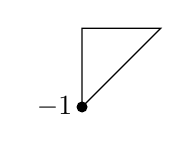
\begin{tikzpicture}
\draw (0,1) -- (0,0) -- (1,1) -- cycle;
\fill (0,0) circle (2pt);
\node[left] at (0,0) {$-1$};
\end{tikzpicture}
\par
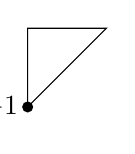
\begin{tikzpicture}[trim left]
\draw (0,1) -- (0,0) -- (1,1) -- cycle;
\fill (0,0) circle (2pt);
\node[left] at (0,0) {$-1$};
\end{tikzpicture}
\end{minipage}}




\subsection{设置图的底线位置}

通常,图的下端底线与两侧文字的基线平齐。baseline 选项设置图的底线与文字基线之间的距离。
\begin{lstlisting}
baseline=<dimension or coordinate or default> 该选项的 dimension 从 x 轴算起,
默认长度单位为 pt。若 dimension 为负数则基线从 x 轴下移。默认以 x 轴为基线。
coordinate 该选项指定基线通过该坐标。
baseline=default  使用默认值,基线在 x 轴上。
\end{lstlisting}

\noindent{\begin{minipage}{9cm}
\begin{lstlisting}
Top align:
\tikz[baseline=(current bounding box.north)]
\draw (0,0) rectangle (1cm,2ex);
\end{lstlisting}
\end{minipage} 
\hspace{1cm}
Top align:
\tikz[baseline=(current bounding box.north)]
\draw (0,0) rectangle (1cm,2ex);
}




\subsection{用 scope 环境或 scoped 命令嵌入图形 }

用这个环境或命令可以在 \verb!{tikzpicture}!环境或 \verb!\tikz!命令之内嵌入子图形。
\begin{lstlisting}
环境格式
\begin{scope}[<options>]
<environment contents>
\end{scope}

命令格式
\usetikzlibrary{scopes}  % 在导言区调用 scopes 程序库
\scoped[<options>]<path command>
\end{lstlisting}

例如\\
{\begin{minipage}{9cm}
\begin{lstlisting}
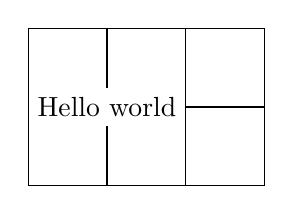
\begin{tikzpicture}
\node [fill=white] at (1,1) {Hello world};
\scoped [on background layer]
\draw (0,0) grid (3,2);
\end{tikzpicture}
\end{lstlisting}
\end{minipage} 
\hspace{1cm}
\begin{minipage}{5cm}
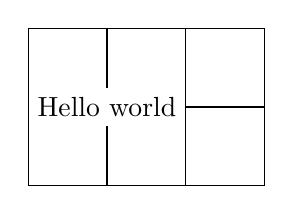
\begin{tikzpicture}
\node [fill=white] at (1,1) {Hello world};
\scoped [on background layer]
\draw (0,0) grid (3,2);
\end{tikzpicture}
\end{minipage}}




\subsection{全局选项设置语句以及 /.style 与 /.default 的设置 }

\begin{lstlisting}
\tikzset{<options>} 全局设置,影响整个分组
my style/.style={<options>} 定义名称为 my style 的样式
hkeyi/.default=<value> 设置名称为 hkeyi 的对象的默认值
\end{lstlisting}

例如,网格对象 help lines 是预定义的,其网格线宽的初始值是 line width=0.2pt,gray,可以用上述选项修改它。\\ 
{\begin{minipage}{12cm}
\begin{lstlisting}
\tikzset{help lines/.style=very thin} % 设置线宽为 very thin。
\tikzset{Karl’s grid/.style={help lines,color=blue!50}} 
% 定义名称为 Karl’s grid 的样式,样式内容是网格 help lines,
% 并设置网格线的颜色是 50% 的蓝色。
\draw[Karl’s grid] (0,0) grid (3,3);
\end{lstlisting}
\end{minipage} 
\hspace{1cm}
\begin{minipage}{5cm}
\tikzset{help lines/.style=very thin}
\tikzset{Karl’s grid/.style={help lines,color=blue!50}}
\tikz \draw [Karl’s grid] (0,0) grid (3,3);
\end{minipage} }

“/.style” 的选项可以带一个变量,用 \#1 表示,例如\\
{\begin{minipage}{12cm}
\begin{lstlisting}
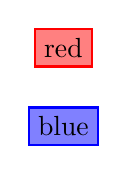
\begin{tikzpicture}[outline/.style={draw=#1,thick,fill=#1!50}]
\node [outline=red] at (0,1) {red};
\node [outline=blue] at (0,0) {blue};
\end{tikzpicture}
\end{lstlisting}
\end{minipage} 
\hspace{1cm}
\begin{minipage}{2cm}
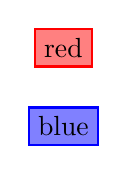
\begin{tikzpicture}[outline/.style={draw=#1,thick,fill=#1!50}]
\node [outline=red] at (0,1) {red};
\node [outline=blue] at (0,0) {blue};
\end{tikzpicture}
\end{minipage} }

\noindent{\begin{minipage}{12cm}
\begin{lstlisting}
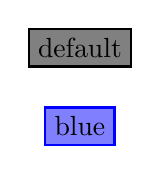
\begin{tikzpicture}[outline/.style={draw=#1,thick,fill=#1!50},
outline/.default=black]
\node [outline] at (0,1) {default};
\node [outline=blue] at (0,0) {blue};
\end{tikzpicture}
\end{lstlisting}
\end{minipage} 
\hspace{1cm}
\begin{minipage}{2cm}
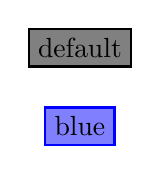
\begin{tikzpicture}[outline/.style={draw=#1,thick,fill=#1!50},
outline/.default=black]
\node [outline] at (0,1) {default};
\node [outline=blue] at (0,0) {blue};
\end{tikzpicture}
\end{minipage}}



\subsection{过指定点的水平线和竖直线 }

\begin{lstlisting}
在导言区调用through程序库 \usetikzlibrary{through},句法
horizontal line through={(<coordinate>)}
vertical line through={(<coordinate>)}
\end{lstlisting}




\section{Path 的相关操作}

\subsection{设置路径样式,在路径中插入路径}

\begin{lstlisting}
命令 \path 将它后面的内容定义为路径,它只能用在{tikzpicture}环境中。
every path/.style={样式定义} 设置环境中所有路径共同的样式(每个路径可以作本地修改)。
insert path=<path> 给路径内部的某个位置添加路径。
\end{lstlisting}

\noindent{\begin{minipage}{10cm}
\begin{lstlisting}
\tikz [c/.style={insert path={circle[radius=4pt]}}]
\draw (0,0) -- (1,1) [c] -- (3,2) [c];
\end{lstlisting}
\end{minipage} 
\hspace{1cm}
\begin{minipage}{5cm}
\tikz [c/.style={insert path={circle[radius=4pt]}}]
\draw (0,0) -- (1,1) [c] -- (3,2) [c];
\end{minipage}}



\subsection{三种路径连接方式以及环路}

Move-To,从路径的前一部分到后一部分没有连线。

Line-To,用直线段连接路径的前一部分与后一部分,用两个短线“\verb!--!”表示。

Curve-To,用曲线(贝塞尔曲线)连接路径的前一部分与后一部分,用两个点“\verb!..!”表示。

--cycle 是环路标识符号。

控制曲线采用如下格式
\begin{lstlisting}
.. controls <first control point> and <second control point> .. <end point>
\end{lstlisting}

例如
\begin{lstlisting}
\draw (0,0) .. controls (1,1) and (2,1) .. (2,0);
\end{lstlisting}
\begin{lstlisting}
\draw (-1,0) .. controls (-1,0.555) and (-0.555,1) .. (0,1)
.. controls (0.555,1) and (1,0.555) .. (1,0);
\end{lstlisting}

曲线也可用以连接 node 的位置
\begin{lstlisting}
\draw [->] (waiting.west) .. controls +(left:5mm) and +(up:5mm)
.. (enter critical.north);
\end{lstlisting}

三种路径连接方式在交接点处有不同的表现,下面是Move-To和Line-To的区别\\
{\begin{minipage}{8cm}
\begin{lstlisting}

\begin{tikzpicture}[line width=10pt]
\draw (0,0) --(1,1) (1,1) --(2,0);
\draw (3,0) -- (4,1) -- (5,0);
\end{tikzpicture}
\end{lstlisting}
\end{minipage} 
\hspace{1cm}
\begin{minipage}{8cm}

\begin{tikzpicture}[line width=10pt]
\draw (0,0) --(1,1) (1,1) --(2,0);
\draw (3,0) -- (4,1) -- (5,0);
\end{tikzpicture}
\end{minipage}}

环路对交接点处的影响如下例\\
{\begin{minipage}{8cm}
\begin{lstlisting}

\begin{tikzpicture}[line width=10pt]
\draw (0,0) -- (1,1) -- (1,0) -- (0,0)
      (2,0) -- (3,1) -- (3,0) -- (2,0);
\draw (5,0) -- (6,1) -- (6,0) -- cycle 
      (7,0) -- (8,1) -- (8,0) -- cycle;
\end{tikzpicture}
\end{lstlisting}
\end{minipage} 
\hspace{0.2cm}
\begin{minipage}{8cm}

\begin{tikzpicture}[line width=10pt]
\draw (0,0) -- (1,1) -- (1,0) -- (0,0)
      (2,0) -- (3,1) -- (3,0) -- (2,0);
\draw (5,0) -- (6,1) -- (6,0) -- cycle 
      (7,0) -- (8,1) -- (8,0) -- cycle;
\end{tikzpicture}
\end{minipage}}



\subsection{用横竖线连接路径部分 }

“\verb!<位置1> | - <位置2>!”表示用过 \verb!<位置1>! 的竖线和过 \verb!<位置2>! 横线把这两个位置连接起来,与 \verb!<位置2> - | <位置1>! 效果一样。这里的 \verb!<位置>! 可以是坐标,也可以是锚位置等。

\noindent{\begin{minipage}{12cm}
\begin{lstlisting}
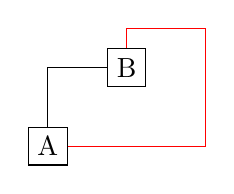
\begin{tikzpicture}
\draw (0,0) node(a) [draw] {A} (1,1) node(b) [draw] {B};
\draw (a.north) |- (b.west);
\draw[color=red] (a.east) -| (2,1.5) -| (b.north);
\end{tikzpicture}
\end{lstlisting}
\end{minipage} 
\hspace{1cm}
\begin{minipage}{3cm}
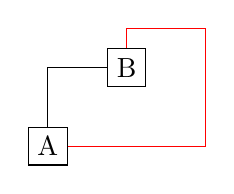
\begin{tikzpicture}
\draw (0,0) node(a) [draw] {A} (1,1) node(b) [draw] {B};
\draw (a.north) |- (b.west);
\draw[color=red] (a.east) -| (2,1.5) -| (b.north);
\end{tikzpicture}
\end{minipage}}



\subsection{连线算子to和edge}
参考node。


\subsection{常用路径选项,命名、颜色、线型等}

\begin{lstlisting}
name path=<name> 给路径命名
\end{lstlisting}
\begin{lstlisting}
color 路径使用默认颜色
color=<color name> 给路径设置颜色
\end{lstlisting}
\begin{lstlisting}
draw 画出路径
draw=<color name> 定义画笔颜色
draw=none 不画路径
\end{lstlisting}
\begin{lstlisting}
line width=<dimension> 定义线宽,初始值 0.4pt
\end{lstlisting}
\begin{lstlisting}
预定义的线宽,由细到粗依次是 
ultra thin,very thin,thin,semithick,thick,very thick,ultra thick
\end{lstlisting}
\begin{lstlisting}
line cap=<type> 定义线端头样式,初始值 butt, 可选round, rect 或 butt
\end{lstlisting}
\begin{lstlisting}
line join=<type> 定义两线交接处的样式,初始值 miter, 可选round, bevel, miter
miter limit=<factor> 初始值 10
\end{lstlisting}
\begin{lstlisting}
dash pattern=<dash pattern>, dash phase=<dash phase>,
预定义的线条样式
solid,dotted,densely dotted,loosely dotted,dashed,densely dashed,loosely dashed,
dash dot,densely dash dot,loosely dash dot,dash dot dot,densely dash dot dot,
loosely dash dot dot
\end{lstlisting}
\begin{lstlisting}
double 设置路径为双线
double=<core color> 设置双线中的第二条线的颜色
double distance=<dimension> 设置双线的间距
\end{lstlisting}
\begin{lstlisting}
fill=<color> 设置填充区域的颜色
fill=none 不填充颜色
\end{lstlisting}
\begin{lstlisting}
pattern=<name> 设置样式线条,需要调用 patterns 程序库
pattern color=<color> 设置样式线条的颜色
\end{lstlisting}
\begin{lstlisting}
decorate 启用装饰样式,需调用相应程序库
decoration=<style> 设置装饰样式,需调用 decoration 程序库
\end{lstlisting}
\begin{lstlisting}
shade 启用颜色渐变效果
shading=<name> 设置颜色渐变的样式,需要调用 shadings 程序库。
\end{lstlisting}
\begin{lstlisting}
shadow 启用阴影,需要调用 shadows 程序库
\end{lstlisting}



\subsection{剪贴命令 clip }

用矩形剪贴\\
{\begin{minipage}{12cm}
\begin{lstlisting}
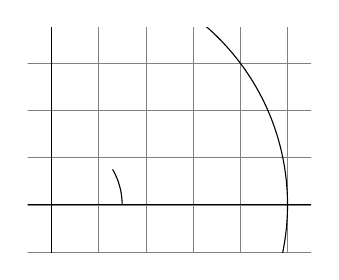
\begin{tikzpicture}[scale=3]
\clip (-0.1,-0.2) rectangle (1.1,0.75);
\draw[step=.2cm,gray,very thin] (-1.4,-1.4) grid (1.4,1.4);
\draw (-1.5,0) -- (1.5,0);
\draw (0,-1.5) -- (0,1.5);
\draw (0,0) circle [radius=1cm];
\draw (3mm,0mm) arc [start angle=0, end angle=30, radius=3mm];
\end{tikzpicture}
\end{lstlisting}
\end{minipage} 
\hspace{0.5cm}
\begin{minipage}{5cm}
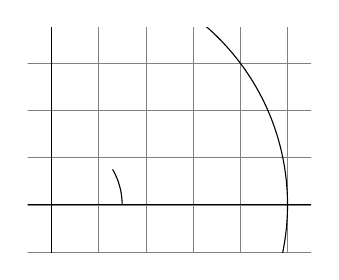
\begin{tikzpicture}[scale=3]
\clip (-0.1,-0.2) rectangle (1.1,0.75);
\draw[step=.2cm,gray,very thin] (-1.4,-1.4) grid (1.4,1.4);
\draw (-1.5,0) -- (1.5,0);
\draw (0,-1.5) -- (0,1.5);
\draw (0,0) circle [radius=1cm];
\draw (3mm,0mm) arc [start angle=0, end angle=30, radius=3mm];
\end{tikzpicture}
\end{minipage}}

用圆形剪贴\\
{\begin{minipage}{12cm}
\begin{lstlisting}
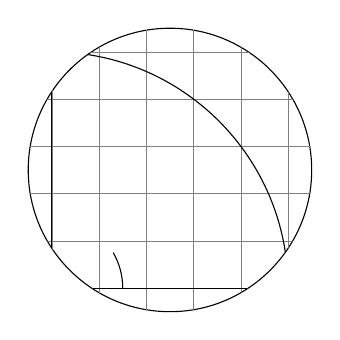
\begin{tikzpicture}[scale=3]
\clip[draw] (0.5,0.5) circle (.6cm);
\draw[step=.2cm,gray,very thin] (-1.4,-1.4) grid (1.4,1.4);
\draw (-1.5,0) -- (1.5,0);
\draw (0,-1.5) -- (0,1.5);
\draw (0,0) circle [radius=1cm];
\draw (3mm,0mm) arc [start angle=0, end angle=30, radius=3mm];
\end{tikzpicture}
\end{lstlisting}
\end{minipage} 
\hspace{0.5cm}
\begin{minipage}{5cm}
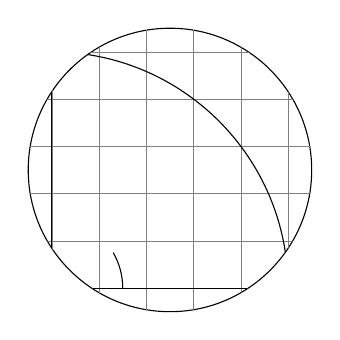
\begin{tikzpicture}[scale=3]
\clip[draw] (0.5,0.5) circle (.6cm);
\draw[step=.2cm,gray,very thin] (-1.4,-1.4) grid (1.4,1.4);
\draw (-1.5,0) -- (1.5,0);
\draw (0,-1.5) -- (0,1.5);
\draw (0,0) circle [radius=1cm];
\draw (3mm,0mm) arc [start angle=0, end angle=30, radius=3mm];
\end{tikzpicture}
\end{minipage}}



\subsection{填充颜色}

颜色填充规则
\begin{itemize}
\item nonzero rule,这是默认填色规则;为了确定点A是否属于被填充的区域,考虑从A出发的射线$\vec l$,并从0开始计数;如果$\vec l$与区域的边界相交且边界从$\vec l$左侧穿到右侧,则计数加1,否则计数减1;若计数结果非0,则点A属于该区域,否则不属于该区域。
\item even odd rule,与上一规则做法类似,如果$\vec l$与区域边界相交的次数是奇数,则点A属于该区域,否则不属于该区域。
\end{itemize}

用 \verb!\fill! 命令填充颜色\\
{\begin{minipage}{10cm}
\begin{lstlisting}
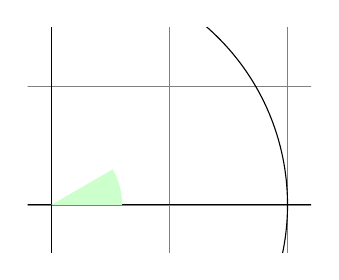
\begin{tikzpicture}[scale=3]
\clip (-0.1,-0.2) rectangle (1.1,0.75);
\draw[step=.5cm,gray,very thin] 
      (-1.4,-1.4) grid (1.4,1.4);
\draw (-1.5,0) -- (1.5,0);
\draw (0,-1.5) -- (0,1.5);
\draw (0,0) circle [radius=1cm];
\fill[green!20!white] (0,0) -- (3mm,0mm)
     arc [start angle=0, end angle=30, radius=3mm]
      -- (0,0);
\end{tikzpicture}
\end{lstlisting}
\end{minipage} 
\hspace{1cm}
\begin{minipage}{6cm}
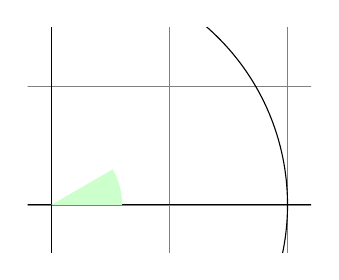
\begin{tikzpicture}[scale=3]
\clip (-0.1,-0.2) rectangle (1.1,0.75);
\draw[step=.5cm,gray,very thin] (-1.4,-1.4) grid (1.4,1.4);
\draw (-1.5,0) -- (1.5,0);
\draw (0,-1.5) -- (0,1.5);
\draw (0,0) circle [radius=1cm];
\fill[green!20!white] (0,0) -- (3mm,0mm)
arc [start angle=0, end angle=30, radius=3mm] -- (0,0);
\end{tikzpicture}
\end{minipage}}

符号green!20!white的意思是绿色占 20\%、白色占 80\%。上面最后的代码可以用 -- cycle 结尾:
\begin{lstlisting}
\fill[green!20!white] (0,0) -- (3mm,0mm)
      arc [start angle=0, end angle=30, radius=3mm] -- cycle;
\end{lstlisting}

\verb!\filldraw!命令先画出路径,然后填充颜色\\
{\begin{minipage}{12cm}
\begin{lstlisting}
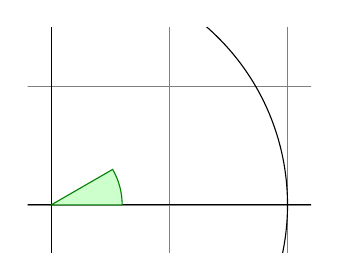
\begin{tikzpicture}[scale=3]
\clip (-0.1,-0.2) rectangle (1.1,0.75);
\draw[step=.5cm,gray,very thin] (-1.4,-1.4) grid (1.4,1.4);
\draw (-1.5,0) -- (1.5,0);
\draw (0,-1.5) -- (0,1.5);
\draw (0,0) circle [radius=1cm];
\filldraw [fill=green!20!white, draw=green!50!black] 
          (0,0) -- (3mm,0mm)
          arc [start angle=0, end angle=30, 
              radius=3mm] -- cycle;
\end{tikzpicture}
\end{lstlisting}
\end{minipage} 
\hspace{0.5cm}
\begin{minipage}{5cm}
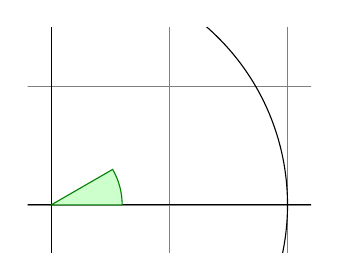
\begin{tikzpicture}[scale=3]
\clip (-0.1,-0.2) rectangle (1.1,0.75);
\draw[step=.5cm,gray,very thin] (-1.4,-1.4) grid (1.4,1.4);
\draw (-1.5,0) -- (1.5,0);
\draw (0,-1.5) -- (0,1.5);
\draw (0,0) circle [radius=1cm];
\filldraw[fill=green!20!white, draw=green!50!black] (0,0) -- (3mm,0mm)
arc [start angle=0, end angle=30, radius=3mm] -- cycle;
\end{tikzpicture}
\end{minipage}}



\subsection{颜色渐变}

颜色渐变命令\verb=\shade=和\verb=\shadedraw=\\
{\begin{minipage}{12cm}
\begin{lstlisting}
\tikz \shade (0,0) rectangle (2,1) (3,0.5) circle (.5cm);
\end{lstlisting}
\end{minipage} 
\hspace{1cm}
\begin{minipage}{5cm}
\tikz \shade (0,0) rectangle (2,1) (3,0.5) circle (.5cm);
\end{minipage}}

默认的是由灰色到白的渐变。如下选择颜色渐变\\
{\begin{minipage}{10cm}
\begin{lstlisting}

\begin{tikzpicture}[rounded corners,ultra thick]
\shade [top color=yellow,bottom color=black] 
       (0,0) rectangle +(2,1);
\shade [left color=yellow,right color=black] 
       (3,0) rectangle +(2,1);
\shadedraw [inner color=yellow,outer color=black,
           draw=yellow] (6,0) rectangle +(2,1);
\shade[ball color=green] (9,.5) circle (.5cm);
\end{tikzpicture}
\end{lstlisting}
\end{minipage} \\
\begin{minipage}{12cm}

\begin{tikzpicture}[rounded corners,ultra thick]
\shade[top color=yellow,bottom color=black] (0,0) rectangle +(2,1);
\shade[left color=yellow,right color=black] (3,0) rectangle +(2,1);
\shadedraw[inner color=yellow,outer color=black,draw=yellow] (6,0) rectangle +(2,1);
\shade[ball color=green] (9,.5) circle (.5cm);
\end{tikzpicture}
\end{minipage}}



\subsection{用 + 表示的平移}

平移 ++(acm, bcm) 是将紧邻此符号之前的点加上向量 (acm, bcm)\\
{\begin{minipage}{10cm}
\begin{lstlisting}
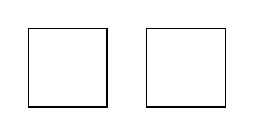
\begin{tikzpicture}
\def\rectanglepath{-- ++(1cm,0cm) -- ++(0cm,1cm) -- 
                   ++(-1cm,0cm) -- cycle}
\draw (0,0) \rectanglepath;
\draw (1.5,0) \rectanglepath;
\end{tikzpicture}
\end{lstlisting}
\end{minipage} 
\hspace{1cm}
\begin{minipage}{5cm}
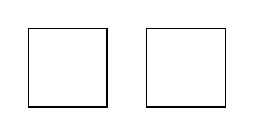
\begin{tikzpicture}
\def\rectanglepath{-- ++(1cm,0cm) -- ++(0cm,1cm) -- ++(-1cm,0cm) -- cycle}
\draw (0,0) \rectanglepath;
\draw (1.5,0) \rectanglepath;
\end{tikzpicture}
\end{minipage}}

上面的小方形可以简化为:\\
{\begin{minipage}{12cm}
\begin{lstlisting}
\tikz \draw (0,0) rectangle +(1,1) (1.5,0) rectangle +(1,1);
\end{lstlisting}
\end{minipage} 
\hspace{0.5cm}
\begin{minipage}{5cm}
\tikz \draw (0,0) rectangle +(1,1) (1.5,0) rectangle +(1,1);
\end{minipage}}

平移 +(acm, bcm) 是将最初的(不是紧邻的)起始点加上向量 (acm, bcm)\\
{\begin{minipage}{12cm}
\begin{lstlisting}
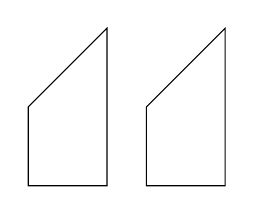
\begin{tikzpicture}
\def\rectanglepath{-- +(1cm,0cm) -- +(1cm,2cm) -- 
                   +(0cm,1cm) -- cycle}
\draw (0,0) \rectanglepath;
\draw (1.5,0) \rectanglepath;
\end{tikzpicture}
\end{lstlisting}
\end{minipage} 
\hspace{1cm}
\begin{minipage}{5cm}
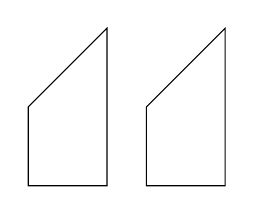
\begin{tikzpicture}
\def\rectanglepath{-- +(1cm,0cm) -- +(1cm,2cm) -- +(0cm,1cm) -- cycle}
\draw (0,0) \rectanglepath;
\draw (1.5,0) \rectanglepath;
\end{tikzpicture}
\end{minipage}}



\section{基本的坐标计算,用比例确定点}

在导言区设置 \verb!\usetikzlibrary{calc}! 调用程序库 calc,然后对坐标做基本计算。

句法格式
\begin{lstlisting}
([<options>]$<coordinate computation>$)
\end{lstlisting}
数乘向量必须加 * 号;必须是小数乘向量这种简单的运算,更复杂的运算,比如,分数或函数表达式乘以向量都是无法计算的。
\begin{lstlisting}
<coordinate>!<number>!<angle>:<second coordinate>
\end{lstlisting}
其中“!<angle>:”可以没有;但如果有“!<angle>:”,则“!<number>”必须有。

表达式\verb.($ (A)!x!(B) $).确定直线AB上一个点,该点与点A的距离比上AB的长度就是x;如果x大于0,该点在射线AB上;如果x小于0,该点在射线BA上,且点A介于该点与点B之间。

表达式\verb.($ (X) ! {sin(60)*2} ! 90:(B) $).指示以X为基点,将线段XB绕X旋转90度,再伸长sin(60)*2倍后,得到的线段端点。

表达式\verb&($ (A) ! .5 ! (B) ! {sin(60)*2} ! 90:(B) $)&指示先运算
\verb&($ (A)!.5!(B) $)&得到一个点,然后该点参与后面的运算。

表达式\verb&($ (A) ! (B) ! (C) $)&指示点B在直线AC上的正交射影点(垂足)。\\
{\begin{minipage}{12cm}
\begin{lstlisting}
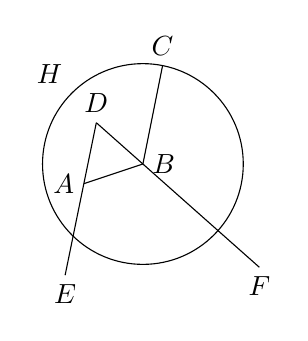
\begin{tikzpicture}
\coordinate [label=left:$A$] (A) at (0,0);
\coordinate [label=right:$B$] (B) at (0.75,0.25);
\coordinate [label=above:$C$] (C) at (1,1.5);
\draw (A) -- (B) -- (C);
\coordinate [label=above:$D$] (D) 
            at ($ (A) ! .5 ! (B) ! {sin(60)*2} ! 90:(B) $) {};
\node (H) [label=135:$H$,draw,circle through=(C)] at (B) {};
\draw (D) -- ($ (D) ! 3.5 ! (B) $) 
             coordinate [label=below:$F$] (F);
\draw (D) -- ($ (D) ! 2.5 ! (A) $) 
             coordinate [label=below:$E$] (E);
\end{tikzpicture}
\end{lstlisting}
\end{minipage} 
\hspace{1cm}
\begin{minipage}{4cm}
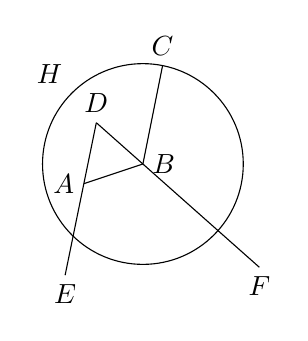
\begin{tikzpicture}
\coordinate [label=left:$A$] (A) at (0,0);
\coordinate [label=right:$B$] (B) at (0.75,0.25);
\coordinate [label=above:$C$] (C) at (1,1.5);
\draw (A) -- (B) -- (C);
\coordinate [label=above:$D$] (D) at
($ (A) ! .5 ! (B) ! {sin(60)*2} ! 90:(B) $) {};
\node (H) [label=135:$H$,draw,circle through=(C)] at (B) {};
\draw (D) -- ($ (D) ! 3.5 ! (B) $) coordinate [label=below:$F$] (F);
\draw (D) -- ($ (D) ! 2.5 ! (A) $) coordinate [label=below:$E$] (E);
\end{tikzpicture}
\end{minipage}}

\noindent{\begin{minipage}{10cm}
\begin{lstlisting}
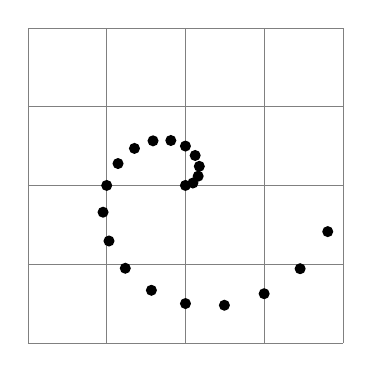
\begin{tikzpicture}
\draw [help lines] (0,0) grid (4,4);
\foreach \i in {0,0.1,...,2}
\fill ($(2,2) !\i! \i*180:(3,2)$) circle (2pt);
\end{tikzpicture}
\end{lstlisting}
\end{minipage} 
\hspace{1cm}
\begin{minipage}{5cm}
\begin{tikzpicture}
\draw [help lines] (0,0) grid (4,4);
\foreach \i in {0,0.1,...,2}
\fill ($(2,2) !\i! \i*180:(3,2)$) circle (2pt);
\end{tikzpicture}
\end{minipage}}

\noindent{\begin{minipage}{11cm}
\begin{lstlisting}
\begin{tikzpicture}
\draw [help lines] (0,0) grid (3,2);
\coordinate (a) at (0,1);
\coordinate (b) at (3,2);
\coordinate (c) at (2.5,0);
\draw (a) node[red,left]{a} -- (b) node[red,right]{b} -- 
      (c) node[red,below]{c} -- cycle;
\draw[red] (a) -- ($(b)!(a)!(c)$);
\draw[orange] (b) -- ($(a)!(b)!(c)$);
\draw[blue] (c) -- ($(a)!(c)!(b)$);
\end{tikzpicture}
\end{lstlisting}
\end{minipage} 
\hspace{1cm}
\begin{minipage}{3cm}
\begin{tikzpicture}
\draw [help lines] (0,0) grid (3,2);
\coordinate (a) at (0,1);
\coordinate (b) at (3,2);
\coordinate (c) at (2.5,0);
\draw (a) node[red,left]{a} -- (b) node[red,right]{b} -- (c) node[red,below]{c} -- cycle;
\draw[red] (a) -- ($(b)!(a)!(c)$);
\draw[orange] (b) -- ($(a)!(b)!(c)$);
\draw[blue] (c) -- ($(a)!(c)!(b)$);
\end{tikzpicture}
\end{minipage}}




\section{交点}

调用intersections程序库,可对交点设置多个选项。选项 name path=\verb!<name>!给当前画的路径命名,用选项 name intersections=\verb!<options>! 给两个路径的交点命名。

name intersections也可带选项
\begin{lstlisting}
name intersections={of=<path1> and <path2>, name=<prefix>, 
              total=<macro>, by={<comma-separated list>}, 
               sort by=<path name>}
\end{lstlisting}
其中,of= 指定两个路径;name= 给交点命名(交点的共名),如果name=i,则这些交点就可用i-1,i-2,i-3这种形式来引用;total=macro,macro是以命令符号 \textbackslash 开头的一组符号,代表交点的总数目;sort by=,按指定路径的方向将交点排序;by=\{comma-separated list\},一组符号或构造对象(个数随意),之间用逗号隔开,用来列举交点;用方括号把 comma-separated list 中列举的对象括起来,方括号内用省略号...,可以按规律自动生成列举项目。

\noindent{\begin{minipage}{11cm}
\begin{lstlisting}
\begin{tikzpicture}
\clip (-2,-2) rectangle (2,2);
\draw [name path=curve 1] (-2,-1) .. controls (8,-1) 
                            and (-8,1) .. (2,1);
\draw [name path=curve 2] (-1,-2) .. controls (-1,8) 
                            and (1,-8) .. (1,2);
\fill [name intersections={
           of=curve 1 and curve 2,
           by={[label=center:a],[label=center:...],
                [label=center:i]}}];
\end{tikzpicture}
\end{lstlisting}
\end{minipage} 
\hspace{1cm}
\begin{minipage}{5cm}
\begin{tikzpicture}
\clip (-2,-2) rectangle (2,2);
\draw [name path=curve 1] (-2,-1) .. controls (8,-1) and (-8,1) .. (2,1);
\draw [name path=curve 2] (-1,-2) .. controls (-1,8) and (1,-8) .. (1,2);
\fill [name intersections={
of=curve 1 and curve 2,
by={[label=center:a],[label=center:...],[label=center:i]}}];
\end{tikzpicture}
\end{minipage}}

\noindent{\begin{minipage}{11cm}
\begin{lstlisting}
\begin{tikzpicture}
\clip (-2,-2) rectangle (2,2);
\draw [name path=curve 1] (-2,-1) .. controls (8,-1) 
                            and (-8,1) .. (2,1);
\draw [name path=curve 2] (-1,-2) .. controls (-1,8) 
                            and (1,-8) .. (1,2);
\fill [name intersections={of=curve 1 and curve 2, 
        name=i,        total=\t}]
      [every node/.style={above left, black, opacity=1},
        red, opacity=0.5]
\foreach \s in {1,...,\t}{(i-\s) circle (2pt) 
            node {\footnotesize\s}};
\end{tikzpicture}
\end{lstlisting}
\end{minipage} 
\hspace{1cm}
\begin{minipage}{5cm}
\begin{tikzpicture}
\clip (-2,-2) rectangle (2,2);
\draw [name path=curve 1] (-2,-1) .. controls (8,-1) 
                            and (-8,1) .. (2,1);
\draw [name path=curve 2] (-1,-2) .. controls (-1,8) 
                            and (1,-8) .. (1,2);
\fill [name intersections={of=curve 1 and curve 2, name=i, total=\t}]
      [every node/.style={above left, black, opacity=1},
        red, opacity=0.5]
\foreach \s in {1,...,\t}{(i-\s) circle (2pt) node {\footnotesize\s}};
\end{tikzpicture}
\end{minipage}}

下图中用了选项 sort by=\verb!\pathname!,所以画了两个图\\
{\begin{minipage}{11cm}
\begin{lstlisting}
\begin{tikzpicture}
\clip (-0.5,-0.75) rectangle (3.25,2.25);
\foreach \pathname/\shift in {line/0cm, curve/2cm}{
\tikzset{xshift=\shift}
\draw [->, name path=curve] (1,1.5) .. controls (-1,1) 
                               and (2,0.5) .. (0,0);
\draw [->, name path=line] (0,-.5) -- (1,2) ;
\fill [name intersections={of=line and curve,
        sort by=\pathname, name=i}]
      [every node/.style={left=.25cm, black, opacity=1},
        red, opacity=0.5]
\foreach \s in {1,2,3}{(i-\s) circle (2pt) 
         node {\footnotesize\s}};
}
\end{tikzpicture}
\end{lstlisting}
\end{minipage} 
\hspace{1cm}
\begin{minipage}{5cm}
\begin{tikzpicture}
\clip (-0.5,-0.75) rectangle (3.25,2.25);
\foreach \pathname/\shift in {line/0cm, curve/2cm}{
\tikzset{xshift=\shift}
\draw [->, name path=curve] (1,1.5) .. controls (-1,1) and (2,0.5) .. (0,0);
\draw [->, name path=line] (0,-.5) -- (1,2) ;
\fill [name intersections={of=line and curve,sort by=\pathname, name=i}]
[red, opacity=0.5, every node/.style={left=.25cm, black, opacity=1}]
\foreach \s in {1,2,3}{(i-\s) circle (2pt) node {\footnotesize\s}};
}
\end{tikzpicture}
\end{minipage}}

\noindent{\begin{minipage}{11.2cm}
\begin{lstlisting}
\begin{tikzpicture}
\coordinate [label=left:$A$] (A) at (0,0);
\coordinate [label=right:$B$] (B) at (1.25,0.25);
\draw [name path=A--B] (A) -- (B);
\node (D) [name path=D,draw,circle through=(B),
             label=left:$D$] 
           at (A) {};
\node (E) [name path=E,draw,circle through=(A),
           label=right:$E$] 
           at (B) {};
\path [name intersections={of=D and E, 
        by={[label=above:$C$]C, [label=below:$C’$]C’} }];
\draw [name path=C--C’,red] (C) -- (C’);
\path [name intersections={of=A--B and C--C’,by=F}];
\node [fill=red,inner sep=1pt,label=-45:$F$] at (F) {};
\end{tikzpicture}
\end{lstlisting}
\end{minipage} 
\hspace{0.3cm}
\begin{minipage}{5cm}
\begin{tikzpicture}
\coordinate [label=left:$A$] (A) at (0,0);
\coordinate [label=right:$B$] (B) at (1.25,0.25);
\draw [name path=A--B] (A) -- (B);
\node (D) [name path=D,draw,circle through=(B),label=left:$D$] at (A) {};
\node (E) [name path=E,draw,circle through=(A),label=right:$E$] at (B) {};
\path [name intersections={of=D and E, by={[label=above:$C$]C, 
         [label=below:$C’$]C’}}];
\draw [name path=C--C’,red] (C) -- (C’);
\path [name intersections={of=A--B and C--C’,by=F}];
\node [fill=red,inner sep=1pt,label=-45:$F$] at (F) {};
\end{tikzpicture}
\end{minipage}}




\section{ 重复操作 }

用含 foreach 的语句实现重复操作,句法
\begin{lstlisting}
\path . . . foreach <variables> [options] in {path commands} . . . ;
上面的 foreach 可用\foreach 代替
\end{lstlisting}

\noindent{\begin{minipage}{7cm}
\begin{lstlisting}
\foreach \x in {1,2,3} {$x =\x$, }
\end{lstlisting}
\end{minipage} 
\hspace{1cm}
\begin{minipage}{4cm}
\foreach \x in {1,2,3} {$x =\x$, }
\end{minipage}}

\noindent{\begin{minipage}{6cm}
\begin{lstlisting}
\tikz \foreach \x in {1,...,10}
\draw (\x,0) circle (0.4cm);
\end{lstlisting}
\end{minipage} 
\hspace{0.5cm}
\begin{minipage}{12cm}
\tikz \foreach \x in {1,...,10}
\draw (\x,0) circle (0.4cm);
\end{minipage}}

下面的数组是以前两项之差为公差的等差数列\\
{\begin{minipage}{7cm}
\begin{lstlisting}
\tikz \foreach \x in {-1,-0.5,...,8}
\draw (\x cm,-1pt) -- (\x cm,1pt);
\end{lstlisting}
\end{minipage} 
\hspace{0.3cm}
\begin{minipage}{12cm}
\tikz \foreach \x in {-1,-0.5,...,8}
\draw [very thick] (\x cm,-5pt) -- (\x cm,5pt);
\end{minipage}}

\noindent{\begin{minipage}{13cm}
\begin{lstlisting}
\tikz \draw (0,0) foreach \x in {1,...,3} { -- (\x,1) -- (\x,0) };
\end{lstlisting}
\end{minipage} 
\hspace{0.3cm}
\begin{minipage}{4cm}
\tikz \draw (0,0) foreach \x in {1,...,3} { -- (\x,1) -- (\x,0) };
\end{minipage}}




\section{node 绘图}

\subsection{node 的句法}

\begin{lstlisting}
\path . . . (<coordinate>) node [<options>](<name>)
            {<node contents>} . . . ;
\end{lstlisting}
node 前面的坐标是它指向的对象,方括号里是选项,圆括号里是 node 的名称(可以不命名),花括号里是内容,但即使无内容也不能省略花括号,选项中含 node contents=\verb!<node contents>! 时可省略花括号及其中的内容。

可用 at 指示 node 指向的位置。
\begin{lstlisting}
\path . . . node [<options>](<name>)
                at(<coordinate>){<node contents>} . . . ;
\end{lstlisting}

可以将 \verb!\path . . . node! 简略为 \verb!\node! 命令,其中 at 可省略
\begin{lstlisting}
\node [<options>](<name>) (<coordinate>)
            {<node contents>} . . . ;
\end{lstlisting}

\noindent{\begin{minipage}{9cm}
\begin{lstlisting}
\begin{tikzpicture}
\path (0,2) node [shape=circle,draw] {(0,2)}
       ( 1,2) node [draw] {(1,2)};
\end{tikzpicture}
\end{lstlisting}
\end{minipage} 
\hspace{1cm}
\begin{minipage}{3cm}
\begin{tikzpicture}
\path (0,2) node [shape=circle,draw] {(0,2)}
       ( 1,2) node [draw] {(1,2)};
\end{tikzpicture}
\end{minipage}}

\noindent{\begin{minipage}{7.5cm}
\begin{lstlisting}
\begin{tikzpicture}
\node at ( 0,2) [circle,draw] {(0,2)};
\end{tikzpicture}
\end{lstlisting}
\end{minipage} 
\hspace{1cm}
\begin{minipage}{3cm}
\begin{tikzpicture}
\node at ( 0,2) [circle,draw] {(0,2)};
\end{tikzpicture}
\end{minipage}}




\subsection{node 的常用选项}

\begin{lstlisting}
shape=<shape name> 选择 coordinate,circle,ellipse,diamond,dart 等形状。初始形状是 rectangle,“shape=”可省略;如果名称为 x 的 node 选择了 coordinate 形状,就可以把它当作 coordinate (x) 来利用,即把它看成坐标。
\end{lstlisting}
\begin{lstlisting}
draw  画出形状的边界
\end{lstlisting}
\begin{lstlisting}
fill  填充颜色
\end{lstlisting}
\begin{lstlisting}
label  给 node 加标签
\end{lstlisting}
\begin{lstlisting}
behind path  指示路径可能会遮挡 node (如果二者有重叠)
in front of path  意思与上相反
\end{lstlisting}
\begin{lstlisting}
double  边界线是双线
\end{lstlisting}
\begin{lstlisting}
rounded corners  边界上的角是圆角
\end{lstlisting}
\begin{lstlisting}
rounded corners=<dimension>   设置边界圆角的半径
\end{lstlisting}
\begin{lstlisting}
inner sep=<dimension>  设置 node 的文字内容与边界的距离
\end{lstlisting}
\begin{lstlisting}
minimum height=<dimension>  设置 node 的最小高度
\end{lstlisting}
\begin{lstlisting}
minimum width=<dimension>
minimum size=<dimension>
shape aspect=<aspect ratio>  设置 node 的宽高之比
\end{lstlisting}
\begin{lstlisting}
shape border rotate=<angle>  使得 node 按指定角度旋转
\end{lstlisting}
\begin{lstlisting}
name=<name>  设置 node 的名称,可以改为上面句法中的命名方法
\end{lstlisting}




\subsection{在 node 中使用 foreach 语句}

举例如下\\
{\begin{minipage}{7.5cm}
\begin{lstlisting}
\tikz \node foreach \x in {1,...,4} 
            foreach \y in {1,2,3}
            [draw] at (\x,\y) {\x,\y};
\end{lstlisting}
\end{minipage} 
\hspace{1cm}
\begin{minipage}{6cm}
\tikz \node foreach \x in {1,...,4} foreach \y in {1,2,3}
[draw] at (\x,\y) {\x,\y};
\end{minipage}}

\noindent{\begin{minipage}{10cm}
\begin{lstlisting}
\tikzstyle{every node}=[dart, inner sep=1pt, draw]
\tikz \node foreach \a/\b/\c in 
                   {A/0/0, B/45/0, C/0/45, D/45/45}
           [shape border rotate=\b, rotate=\c] 
           at (\b/36,-\c/36) {\a};
\end{lstlisting}
\end{minipage} 
\hspace{1cm}
\begin{minipage}{4cm}
{\tikzstyle{every node}=[dart, inner sep=1pt, draw]
\tikz \node foreach \a/\b/\c in {A/0/0, B/45/0, C/0/45, D/45/45}
[shape border rotate=\b, rotate=\c] at (\b/36,-\c/36) {\a};}
\end{minipage}}




\subsection{为环境内所有 node 设置样式}

\begin{lstlisting}
every <shape> node/.style={style}
\end{lstlisting}
环境的这个选项可以为环境内的每个形状为 \verb!<shape>!(如果无此形状选项,就针对所有 node)的 node 设置相同的基本样式,各个 node 可以在这个基本样式的基础上再分别修改。

\noindent{\begin{minipage}{9cm}
\begin{lstlisting}
\begin{tikzpicture}[every node/.style={draw}]
\draw (0,0) node {A} -- (1,1) node {B};
\end{tikzpicture}
\end{lstlisting}
\end{minipage} 
\hspace{1cm}
\begin{minipage}{2cm}
\begin{tikzpicture}[every node/.style={draw}]
\draw (0,0) node {A} -- (1,1) node {B};
\end{tikzpicture}
\end{minipage}}

\noindent{\begin{minipage}{11.5cm}
\begin{lstlisting}
\begin{tikzpicture}
      [every rectangle node/.style={draw},
        every circle node/.style={draw,double}]
\draw (0,0) node[rectangle] {A} -- (1,1) node[circle] {B};
\end{tikzpicture}
\end{lstlisting}
\end{minipage} 
\hspace{1cm}
\begin{minipage}{2cm}
\begin{tikzpicture}
[every rectangle node/.style={draw},
every circle node/.style={draw,double}]
\draw (0,0) node[rectangle] {A} -- (1,1) node[circle] {B};
\end{tikzpicture}
\end{minipage}}

\begin{lstlisting}
name prefix=<text>
\end{lstlisting}
环境的这个选项可以为环境内的所有 node 的名称设置相同的前缀,即“共名”,以便于引用,观察下例,注意其中前缀之后加短线 \verb!-!\\
{\begin{minipage}{8.2cm}
\begin{lstlisting}
\tikz {
       \begin{scope}[name prefix = top-]
       \node (A) at (0,1) {A};
       \node (B) at (1,1) {B};
       \draw (A) -- (B);
       \end{scope}
       \begin{scope}[name prefix = bottom-]
       \node (A) at (0,0) {A};
       \node (B) at (1,0) {B};
       \draw (A) -- (B);
       \end{scope}
       \draw [red] (top-A) -- (bottom-B);
        }
\end{lstlisting}
\end{minipage} 
\hspace{1cm}
\begin{minipage}{2cm}
\tikz {
\begin{scope}[name prefix = top-]
\node (A) at (0,1) {A};
\node (B) at (1,1) {B};
\draw (A) -- (B);
\end{scope}
\begin{scope}[name prefix = bottom-]
\node (A) at (0,0) {A};
\node (B) at (1,0) {B};
\draw (A) -- (B);
\end{scope}
\draw [red] (top-A) -- (bottom-B);
}
\end{minipage}}




\subsection{node 中的文字编辑}

在node中的文字有多个选项
\begin{lstlisting}
text=<color> 设置文字颜色
\end{lstlisting}
\begin{lstlisting}
node font=<font commands> 设置 node 的所有字体
\end{lstlisting}
\begin{lstlisting}
font=<font commands> 设置 node 的花括号内的字体
\end{lstlisting}

例如\\
{\begin{minipage}{12.5cm}
\begin{lstlisting}
\begin{tikzpicture}
\draw[node font=\itshape] (1,0) -- +(1,1) node[above] {italic};
\end{tikzpicture}
\end{lstlisting}
\end{minipage} 
\hspace{1cm}
\begin{minipage}{2cm}
\begin{tikzpicture}
\draw[node font=\itshape] (1,0) -- +(1,1) node[above] {italic};
\end{tikzpicture}
\end{minipage}}



\subsection{可以在 node 的内容中插入环境}

例如插入 \LaTeX 的 tabular 环境\\
{\begin{minipage}{6.2cm}
\begin{lstlisting}
\tikz \node [draw] {
\begin{tabular}{cc}
      upper left & upper right\\
      lower left & lower right
\end{tabular}
                    };
\end{lstlisting}
\end{minipage} 
\hspace{1cm}
\begin{minipage}{5cm}
\tikz \node [draw] {
\begin{tabular}{cc}
upper left & upper right\\
lower left & lower right
\end{tabular}
};
\end{minipage}}



\subsection{node 的文字对齐方式}

可以用如下选项选择 node 内容中文字对齐方式
\begin{lstlisting}
align=center
align=right
align=flush left
align=flush center
align=justify
\end{lstlisting}

\noindent{\begin{minipage}{12cm}
\begin{lstlisting}
\tikz[align=center] \node[draw] {This is a\\demonstration.};
\end{lstlisting}
\end{minipage} 
\hspace{1cm}
\begin{minipage}{3cm}
\tikz[align=center] \node[draw] {This is a\\demonstration.};
\end{minipage}}

\noindent{\begin{minipage}{12cm}
\begin{lstlisting}
\tikz \node[fill=yellow!80!black,align=right]
{This is a\\[-2pt] demonstration text for\\[1ex] alignments.};
\end{lstlisting}
\end{minipage} 
\hspace{0.2cm}
\begin{minipage}{5cm}
\tikz \node[fill=yellow!80!black,align=right]
{This is a\\[-2pt] demonstration text for\\[1ex] alignments.};
\end{minipage}}

\noindent{\begin{minipage}{13.3cm}
\begin{lstlisting}
\tikz \node[fill=yellow!80!black,text width=3cm,align=flush center]
{This is a demonstration text for showing how line breaking works.};
\end{lstlisting}
\end{minipage} 
\hspace{0.2cm}
\begin{minipage}{3cm}
\tikz \node[fill=yellow!80!black,text width=3cm,align=flush center]
{This is a demonstration text for showing how line breaking works.};
\end{minipage}}



\subsection{设置 node 每行文字的最大宽度}

可用选项 text width=\verb!<dimension>!设置 node 每行文字的最大宽度\\
{\begin{minipage}{13.3cm}
\begin{lstlisting}
\tikz \draw (0,0) node[fill=yellow!80!black,text width=3cm]
{This is a demonstration text for showing how line breaking works.};
\end{lstlisting}
\end{minipage} 
\hspace{0.2cm}
\begin{minipage}{3cm}
\tikz \draw (0,0) node[fill=yellow!80!black,text width=3cm]
{This is a demonstration text for showing how line breaking works.};
\end{minipage}}




\subsection{node 的锚位置 }

node 指向的对象可以是坐标、node、路径等,这些对象都有以下位置
\begin{itemize}
\item 中心, center
\item 罗盘位置,north,north east,east,south east,
    south,south west,west,north west,罗盘位置都在对象的边界上
\item 基线位置,base,base west,base east
\item 中间水平线位置,mid,mid west,mid east
\item 后缀标记方位,如果对象名称为(u),还可用后缀标记方位 u.north,u.north east,u.south west,u.center 等
\end{itemize}

锚(anchor)位置选项的格式是 anchor=\verb!<anchor name>!,指示 node 的“锚”放在对象的 \verb!<anchor name>!位置,注意“锚与船的位置总是相对的”,即 node 的显示位置总与指定的锚位相对。

\noindent {\begin{minipage}{12cm}
\begin{lstlisting}
\begin{tikzpicture}
\draw (-0.5,0) rectangle (3.5,3);
\draw (0.5,0.5) node [fill=yellow!80!black, anchor=south west]
              {Text at \verb!node 1!}
       -- (2.5,2.5) node [anchor=east] 
              {Text at \verb!node 2!};
\end{tikzpicture}
\end{lstlisting}
\end{minipage} 
\hspace{1cm}
\begin{minipage}{4cm}
\begin{tikzpicture}
\draw (-0.5,0) rectangle (3.5,3);
\draw (0.5,0.5) node [fill=yellow!80!black, anchor=south west]
{Text at \verb!node 1!}
-- (2.5,2.5) node [anchor=east] {Text at \verb!node 2!};
\end{tikzpicture}
\end{minipage}}




\subsection{node 的平移位置}

\begin{lstlisting}
above 将 node 平移到所指定的对象上部,但仍然在对象的边界线上
below,left,right,
\end{lstlisting}
\begin{lstlisting}
above=<offset> 设置从所指定的对象的中心向上平移的距离
below=<offset>,left=<offset>,right=<offset>
\end{lstlisting}
\begin{lstlisting}
above left,above right,below left,below right
\end{lstlisting}
\begin{lstlisting}
above left=距离1and距离2,从所指定的对象中心算起,上移距离1并左移距离2
above right=距离1and距离2
below left=距离1and距离2
below right=距离1and距离2
\end{lstlisting}
\begin{lstlisting}
centered
\end{lstlisting}

\noindent {\begin{minipage}{12cm}
\begin{lstlisting}
\tikz \fill (0,0) circle (2pt) node[above] {above};
\tikz \fill (0,0) circle (2pt) node[above=10pt] {above};
\end{lstlisting}
\end{minipage} 
\hspace{1cm}
\begin{minipage}{4cm}
\tikz \fill (0,0) circle (2pt) node[above] {above};
\tikz \fill (0,0) circle (2pt) node[above=10pt] {above};
\end{minipage}}




\subsection{设置诸 node 的相互位置}

首先调用 \verb!positioning!程序库。

举例来说
\begin{lstlisting}
\node at (1,1) [above=2,draw] {above};
定义 node 的中心在 (1,1) 之上 2cm 处
\end{lstlisting}
\begin{lstlisting}
\node at (1,1) [above right=.2 and 3mm,draw] {above};
定义 node 的中心在 (1,1) 之上0.2cm,之右3mm处
\end{lstlisting}
\begin{lstlisting}
\node [above=5mm of somenode.north east]
定义 node 的中心在名为 somenode 的 node 的 north east 位置之上 5mm 处,注意必须带 of
\end{lstlisting}

\begin{lstlisting}
\usetikzlibrary{positioning}    % 在导言区设置
\begin{tikzpicture}
      [place/.style={circle,draw=blue!50,fill=blue!20,thick,
         inner sep=0pt,minimum size=6mm},
       transition/.style={rectangle,draw=black!50,fill=black!20,
         thick,inner sep=4pt,minimum size=4mm},
       display/.style={draw=red!50,fill=red!20,thick,
         inner sep=5pt},diamond,aspect=2]
\node[place] (a)  at ( 0,2) {a};
\node[place] (b) [below=of a] {b};
\node[place] (c) [below=of b] {c};
\node[transition] (d) [right=of b] {\huge d};
\node[transition] (e) [left=of b] {e};
\node[display] (f) [above right=of d.north east] {f};
\end{tikzpicture}
\end{lstlisting}
\begin{tikzpicture}
      [place/.style={circle,draw=blue!50,fill=blue!20,thick,
         inner sep=0pt,minimum size=6mm},
       transition/.style={rectangle,draw=black!50,fill=black!20,
         thick,inner sep=4pt,minimum size=4mm},
       display/.style={draw=red!50,fill=red!20,thick,
         inner sep=5pt},diamond,aspect=2]
\node[place] (a)  at ( 0,2) {a};
\node[place] (b) [below=of a] {b};
\node[place] (c) [below=of b] {c};
\node[transition] (d) [right=of b] {\huge d};
\node[transition] (e) [left=of b] {e};
\node[display] (f) [above right=of d.north east] {f};
\end{tikzpicture}

位置选项 above right=3 and 4 指示向上平移3cm,向右平移4cm; above=3 and 4 指示向上平移3cm,没有横向平移,故4无用。

\noindent {\begin{minipage}{10cm}
\begin{lstlisting}
\begin{tikzpicture}
\draw[help lines] (0,0) grid (4,4);
\fill [red](0,0) circle [radius=2pt];
\fill [red](4,3) circle [radius=2pt];
\node (0,0) [below] {$(0,0)$};
\node (4,3) [below left]{$(4,3)$} ;
\node at (0,0) [above right=3 and 4,draw] {above};
\end{tikzpicture}
\end{lstlisting}
\end{minipage} 
\hspace{1cm}
\begin{minipage}{5cm}
\begin{tikzpicture}
\draw[help lines] (0,0) grid (4,4);
\fill [red](0,0) circle [radius=2pt];
\fill [red](4,3) circle [radius=2pt];
\node (0,0) [below] {$(0,0)$};
\node at (4,3) [below left]{$(4,3)$} ;
\node at (0,0) [above right=3 and 4,draw] {above};
\end{tikzpicture}
\end{minipage}}

选项“node distance=距离”确定两个 node 的间距。当环境带有 on grid 选项时,该值指的是 node 的中心之间的距离;当环境无 on grid 选项时,该值指的是 node 边界之间的距离,初始值为1cm。

\noindent {\begin{minipage}{12cm}
\begin{lstlisting}
\begin{tikzpicture}[every node/.style=draw,node distance=5mm]
\draw[help lines] (0,0) grid (2,3);
% Not gridded
\node (a1) at (0,0) {not gridded};
\node (b1) [above=of a1] {fooy};
\node (c1) [above=of b1] {a};
% gridded
\begin{scope}[on grid]
\node (a2) at (2,0) {gridded};
\node (b2) [above=of a2] {fooy};
\node (c2) [above=of b2] {a};
\end{scope}
\end{tikzpicture}
\end{lstlisting}
\end{minipage} 
\hspace{0.5cm}
\begin{minipage}{3cm}
\begin{tikzpicture}[every node/.style=draw,node distance=5mm]
\draw[help lines] (0,0) grid (2,3);
\node (a1) at (0,0) {not gridded};
\node (b1) [above=of a1] {fooy};
\node (c1) [above=of b1] {a};
\begin{scope}[on grid]
\node (a2) at (2,0) {gridded};
\node (b2) [above=of a2] {fooy};
\node (c2) [above=of b2] {a};
\end{scope}
\end{tikzpicture}
\end{minipage}}




\subsection{路径上的 node 标签的位置选项}

把 node 作为标签添加到路径上,通常,node 的位置取决于代码的次序
\begin{lstlisting}
(0,0)node{a} -- (1,1) 把 node 标签加在(0,0)点处
\end{lstlisting}
\begin{lstlisting}
(0,0) --node{a}(1,1) 把 node 标签加在线中间
\end{lstlisting}
\begin{lstlisting}
(0,0) -- (1,1)node{a} 把 node 标签加在(1,1)点处
\end{lstlisting}

也可以用选项调整 node 标签的位置,常用的标签位置选项如下
\begin{lstlisting}
pos=<小数> 
\end{lstlisting}
\begin{lstlisting}
auto,auto=<direction>
swap 或撇号 `
\end{lstlisting}
\begin{lstlisting}
sloped
\end{lstlisting}
\begin{lstlisting}
allow upside down=<boolean>  初始值 false
\end{lstlisting}
\begin{lstlisting}
midway  等于 pos=0.5
\end{lstlisting}
\begin{lstlisting}
near start  等于 pos=0.25
\end{lstlisting}
\begin{lstlisting}
near end  等于 pos=0.75
\end{lstlisting}
\begin{lstlisting}
very near start  等于 pos=0.125
\end{lstlisting}
\begin{lstlisting}
very near end  等于 pos=0.875
\end{lstlisting}
\begin{lstlisting}
at start  等于 pos=0
\end{lstlisting}
\begin{lstlisting}
at end  等于 pos=1
\end{lstlisting}



pos=0指示把 node 标签在起点,pos=1指示把 node 标签在终点\\
\noindent {\begin{minipage}{12cm}
\begin{lstlisting}
\tikz \draw (0,0) -- (3,1)
        node[pos=0]{0} node[pos=0.5]{1/2} node[pos=0.9]{9/10};
\end{lstlisting}
\end{minipage} 
\hspace{1cm}
\begin{minipage}{4cm}
\tikz \draw (0,0) -- (3,1)
node[pos=0]{0} node[pos=0.5]{1/2} node[pos=0.9]{9/10};
\end{minipage}}

\noindent {\begin{minipage}{11cm}
\begin{lstlisting}
\tikz \draw (0,0) .. controls +(right:3.5cm) 
              and +(right:3.5cm) .. (0,3)
        node foreach \p in {0,0.125,...,1} [pos=\p]{\p};
\end{lstlisting}
\end{minipage} 
\hspace{1cm}
\begin{minipage}{4cm}
\tikz \draw (0,0) .. controls +(right:3.5cm) and +(right:3.5cm) .. (0,3)
node foreach \p in {0,0.125,...,1} [pos=\p]{\p};
\end{minipage}}

\noindent {\begin{minipage}{12cm}
\begin{lstlisting}
\tikz \draw (0,0) |- (3,1)
        node[pos=0]{0} node[pos=0.5]{1/2} node[pos=0.9]{9/10};
\end{lstlisting}
\end{minipage} 
\hspace{0.5cm}
\begin{minipage}{1cm}
\tikz \draw (0,0) |- (3,1)
node[pos=0]{0} node[pos=0.5]{1/2} node[pos=0.9]{9/10};
\end{minipage}}

选项 auto 指示 node 标签在线的左侧或右侧(默认是 scope 的设置), auto=left 指示 node 标签在线的左侧, auto=right 指示 node 标签在线的右侧。选项 swap 指示 node 标签放在与 auto 相反的一侧,英文的撇号(一个单引号)'是 swap 的简写。

\noindent {\begin{minipage}{9cm}
\begin{lstlisting}
\begin{tikzpicture}[auto,bend right]
\node (a) at (0:1) {$0^\circ$};
\node (b) at (120:1) {$120^\circ$};
\node (c) at (240:1) {$240^\circ$};
\draw (a) to node {1} node [swap] {1’} (b)
      (b) to node {2} node [swap] {2’} (c)
      (c) to node {3} node [swap] {3’} (a);
\end{tikzpicture}
\end{lstlisting}
\end{minipage} 
\hspace{1cm}
\begin{minipage}{12cm}
\begin{tikzpicture}[auto,bend right]
\node (a) at (0:1) {$0^\circ$};
\node (b) at (120:1) {$120^\circ$};
\node (c) at (240:1) {$240^\circ$};
\draw (a) to node {1} node [swap] {1’} (b)
(b) to node {2} node [swap] {2’} (c)
(c) to node {3} node [swap] {3’} (a);
\end{tikzpicture}
\end{minipage}}

选项 sloped 使得 node 标签沿着路径倾斜\\
\noindent {\begin{minipage}{9cm}
\begin{lstlisting}
\tikz \draw (0,0) .. controls +(up:2cm) 
            and +(left:2cm) .. (1,3)
            node foreach \p in {0,0.25,...,1}
                [sloped,above,pos=\p]{\p};
\end{lstlisting}
\end{minipage} 
\hspace{1cm}
\begin{minipage}{12cm}
\tikz \draw (0,0) .. controls +(up:2cm) and +(left:2cm) .. (1,3)
node foreach \p in {0,0.25,...,1} [sloped,above,pos=\p]{\p};
\end{minipage}}

选项 allow upside down=true 或 allow upside down 使得 node 标签总在路径线的一侧,而不是只在路径线的凸的一侧。\\
\noindent {\begin{minipage}{12cm}
\begin{lstlisting}
\tikz [allow upside down]
\draw (0,0) .. controls +(up:2cm) 
      and +(left:2cm) .. (1,3)
      node foreach \p in {0,0.25,...,1} 
         [sloped,above,pos=\p]{\p};
\end{lstlisting}
\end{minipage} 
\hspace{1cm}
\begin{minipage}{12cm}
\tikz [allow upside down]
\draw (0,0) .. controls +(up:2cm) 
      and +(left:2cm) .. (1,3)
      node foreach \p in {0,0.25,...,1} 
         [sloped,above,pos=\p]{\p};
\end{minipage}}

选项  midway 将 node 标签放在路径中间\\
\noindent {\begin{minipage}{12cm}
\begin{lstlisting}
\begin{tikzpicture}[->]
\draw (0,0) -- (2,0.5) node[midway,sloped,above] {$x$};
\draw (2,-.5) -- (0,0) node[midway,sloped,below] {$y$};
\end{tikzpicture}
\end{lstlisting}
\end{minipage} 
\hspace{1cm}
\begin{minipage}{12cm}
\begin{tikzpicture}[->]
\draw (0,0) -- (2,0.5) node[midway,sloped,above] {$x$};
\draw (2,-.5) -- (0,0) node[midway,sloped,below] {$y$};
\end{tikzpicture}
\end{minipage}}



\subsection{给 node 加 label 标签,label 的用法 }

给 node 加标签可用两种方法,方法一,用\verb!\node!,这个方法已如前所述。方法二,用 label 选项。

label 的句法
\begin{lstlisting}
label=[options]<angle>:<text>
\end{lstlisting}
其中 angle 是标签所指向的对象的方位,可以是角度(方向角,有正负),也可以是 above, below,left,right,above left等等。text是标签内容。

注意下面代码中的 label 的选项要用花括号括起来。\\
\noindent {\begin{minipage}{9.5cm}
\begin{lstlisting}
\tikz
\node [circle, draw,scale=2,
          label=default,
          label={[green]60:\Huge $60^\circ$},
          label=below:$-90^\circ$,
          label=3:$3^\circ$,
          label=2:$2^\circ$,
          label={[green,below]180:$180^\circ$},
          label={[red,centered]135:$115^\circ$}] 
      {\tiny my circle};
\end{lstlisting}
\end{minipage} 
\hspace{0.2cm}
\begin{minipage}{12cm}
\tikz
\node [circle, draw,scale=3,
          label=default,
          label={[green,above right=1 and 2]60:\huge $60^\circ$},
          label={[below=1]below:$-90^\circ$},
          label=3:$3^\circ$,
          label=2:$2^\circ$,
          label={[green,below=2]180:$180^\circ$},
          label={[red,centered]135:$115^\circ$}] 
      {\tiny my circle};
\end{minipage}}

可以给标签命名,加以引用\\
\noindent {\begin{minipage}{8.5cm}
\begin{lstlisting}
\begin{tikzpicture}
\node [circle,draw,label={[name=label node]
        above left:$a,b$}] {};
\draw (label node) -- +(1,1);
\end{tikzpicture}
\end{lstlisting}
\end{minipage} 
\hspace{1cm}
\begin{minipage}{3cm}
\begin{tikzpicture}
\node [circle,draw,label={[name=label node]
         above left:$a,b$}] {};
\draw (label node) -- +(1,1);
\end{tikzpicture}
\end{minipage}}

可用环境选项 every label/.style=\{\} 设置各个 label 的样式\\
\noindent {\begin{minipage}{13cm}
\begin{lstlisting}
\tikz [rotate=-80,every label/.style={draw,red}]
\node [transform shape,rectangle,draw,label=right:label] {main node};
\end{lstlisting}
\end{minipage} 
\hspace{1cm}
\begin{minipage}{12cm}
\tikz [rotate=-80,every label/.style={draw,red}]
\node [transform shape,rectangle,draw,label=right:label] {main node};
\end{minipage}}

选项 label distance 设置标签与对象之间的距离\\
\noindent {\begin{minipage}{7cm}
\begin{lstlisting}
\tikz[label distance=5mm]
\node [circle,draw,label=right:X,
        label=above right:Y,
        label=above:Z] {my circle};
\end{lstlisting}
\end{minipage} 
\hspace{1cm}
\begin{minipage}{12cm}
\tikz[label distance=5mm]
\node [circle,draw,label=right:X,
label=above right:Y,
label=above:Z] {my circle};
\end{minipage}}

\noindent {\begin{minipage}{12cm}
\begin{lstlisting}
\begin{tikzpicture}
      [place/.style={circle,draw=blue!50,fill=blue!20,thick,
      inner sep=0pt,minimum size=6mm}]
\node[place, label=right:$s\le3$] (waiting) at (0,2) {};
\end{tikzpicture}
\end{lstlisting}
\end{minipage} 
\hspace{1cm}
\begin{minipage}{12cm}
\begin{tikzpicture}
      [place/.style={circle,draw=blue!50,fill=blue!20,thick,
      inner sep=0pt,minimum size=6mm}]
\node[place, label={[red]right:$s\le3$}] (waiting) at (0,2) {};
\end{tikzpicture}
\end{minipage}}



\subsection{大头针 pin 标签}

pin 标签的用法与 label 类似,只是多了边的设置。
\begin{lstlisting}
every pin edge/.style={ }
pin edge=<options>
\end{lstlisting}

\noindent {\begin{minipage}{11cm}
\begin{lstlisting}
\tikz [pin distance=15mm,
       every pin edge/.style={<-,shorten <=1pt,decorate,
        decoration={snake,pre length=4pt}}]
\node [circle,draw,pin=right:X,
       pin=above right:Y,
       pin=above:Z] {my circle};
\end{lstlisting}
\end{minipage} 
\hspace{1cm}
\begin{minipage}{12cm}
\tikz [pin distance=15mm,
every pin edge/.style={<-,shorten <=1pt,decorate,
decoration={snake,pre length=4pt}}]
\node [circle,draw,pin=right:X,
pin=above right:Y,
pin=above:Z] {my circle};
\end{minipage}}


\noindent {\begin{minipage}{11cm}
\begin{lstlisting}
\tikz [every pin edge/.style={},
         initial/.style={pin={[pin distance=5mm,
                    pin edge={<-,shorten <=1pt}]
       left:start}}]
\node [circle,draw,initial] {my circle};
\end{lstlisting}
\end{minipage} 
\hspace{1cm}
\begin{minipage}{12cm}
\tikz [every pin edge/.style={},
initial/.style={pin={[pin distance=5mm,
pin edge={<-,shorten <=1pt}]left:start}}]
\node [circle,draw,initial] {my circle};
\end{minipage}}



\subsection{用引用选项 quotes 给 node加标签}

首先调用 quotes 程序库 \verb!\usetikzlibrary{quotes}!。

在 \verb!\node!的选项中,用双引号引起的字符串(不含某些特殊符号)会被作为标签引用。下面两句等效\\
\noindent {\begin{minipage}{11cm}
\begin{lstlisting}
\tikz \node ["my label" red, draw] {my node};
\tikz \node [label={[red]my label}, draw] {my node};
\end{lstlisting}
\end{minipage} 
\hspace{1cm}
\begin{minipage}{12cm}
\tikz \node ["my label" red, draw] {my node};
\end{minipage}}
显然双引号简捷一些。


\noindent {\begin{minipage}{11cm}
\begin{lstlisting}
\begin{tikzpicture} % 调用 matrix 程序库
\matrix [row sep=5mm,column sep=5mm] {
\node [draw, "label"] {A}; &
\node [draw, "label" left] {B}; &
\node [draw, "label" centered] {C}; \\
\node [draw, "label" color=red] {D}; &
\node [draw, "label" {red,draw,thick}] {E} ;&
\node [draw, "label" {green,draw,ultra thick}] {F};\\ };
\end{tikzpicture}
\end{lstlisting}
\end{minipage} 
\hspace{0.2cm}
\begin{minipage}{12cm}
\begin{tikzpicture}
\matrix [row sep=5mm,column sep=5mm] {
\node [draw, "label"] {A}; &
\node [draw, "label" left] {B}; &
\node [draw, "label" centered] {C}; \\
\node [draw, "label" color=red] {D}; &
\node [draw, "label" {red,draw,thick}] {E} ;&
\node [draw, "label" {green,draw,ultra thick}] {F};\\ };
\end{tikzpicture}
\end{minipage}}


\noindent {\begin{minipage}{10cm}
\begin{lstlisting}
\tikz \node ["90:$90^\circ$", "left:$180^\circ$", 
            circle, draw] {circle};
\tikz [every label quotes/.style=red]
      \node ["90:$90^\circ$", "left:$180^\circ$", 
            circle, draw] {circle};
\end{lstlisting}
\end{minipage} 
\hspace{0.5cm}
\begin{minipage}{12cm}
\tikz
\node ["90:$90^\circ$", "left:$180^\circ$", circle, draw] {circle};
\tikz [every label quotes/.style=red]
\node ["90:$90^\circ$", "left:$180^\circ$", circle, draw] {circle};
\end{minipage}}

如果引号内有逗号或冒号,要用花括号括起来。\\
\noindent {\begin{minipage}{8.5cm}
\begin{lstlisting}
\tikz \node ["{yes, we can}", draw] {foo};
\tikz \node ["yes{:} we can", draw] {foo};
\end{lstlisting}
\end{minipage} 
\hspace{1cm}
\begin{minipage}{12cm}
\tikz \node ["{yes, we can}",draw] {foo};
\tikz \node ["yes{:} we can",draw] {foo};
\end{minipage}}




\section{ 在 node 之间画线}

\subsection{用符号 $--$,$..$,$-|$ 画线}

可以在坐标、node 之间画连线。基本线条样式有3种:用 \verb!--! 表示的直线段,用 \verb!..!表示的曲线,用 \verb!-|!或 \verb!|-!表示的直角连线。

连线的起止点可以是坐标,node 的锚位置,node 的名称,带方位后缀的 node 的名称。({  \kaishu \color{red} 参照 \verb!node! 的位置 })


\noindent {\begin{minipage}{11.5cm}
\begin{lstlisting}
\begin{tikzpicture}
\path (0,0) node (x) {Hello World!}
(3,1) node[circle,draw](y) {$\int_1^2 x \mathrm d x$};
\draw[->,blue] (x) -- (y);
\draw[->,red] (x) -| node[near start,below] {label} (y);
\draw[->,orange] (x) .. controls +(up:1cm) and +(left:1cm)
                     .. node[above,sloped] {label} (y);
\end{tikzpicture}
\end{lstlisting}
\end{minipage} 
\hspace{0.2cm}
\begin{minipage}{12cm}
\begin{tikzpicture}
\path (0,0) node (x) {Hello World!}
(3,1) node[circle,draw](y) {$\int_1^2 x \mathrm d x$};
\draw[->,blue] (x) -- (y);
\draw[->,red] (x) -| node[near start,below] {label} (y);
\draw[->,orange] (x) .. controls +(up:1cm) and +(left:1cm)
                     .. node[above,sloped] {label} (y);
\end{tikzpicture}
\end{minipage}}

\noindent {\begin{minipage}{12.2cm}
\begin{lstlisting}
\begin{tikzpicture}
      [place/.style={circle,draw=blue!50,fill=blue!20,thick,
       inner sep=0pt,minimum size=6mm},
       transition/.style={rectangle,draw=black!50,fill=black!20,
       thick,inner sep=0pt,minimum size=4mm}]
\node[place] (a) {a};
\node[place] (b) [below=of a] {b};
\node[transition] (c) [left=of b] {c};
\draw [->] (b.north) -- (a.south);
\draw [->] (b.west) -- (c.east);
\draw [->] (a.west) .. controls +(left:5mm) and +(up:5mm)
            .. (c.north);
\end{tikzpicture}
\end{lstlisting}
\end{minipage} 
\hspace{1cm}
\begin{minipage}{12cm}
\begin{tikzpicture}
      [place/.style={circle,draw=blue!50,fill=blue!20,thick,
       inner sep=0pt,minimum size=6mm},
       transition/.style={rectangle,draw=black!50,fill=black!20,
       thick,inner sep=0pt,minimum size=4mm}]
\node[place] (a) {a};
\node[place] (b) [below=of a] {b};
\node[transition] (c) [left=of b] {c};
\draw [->] (b.north) -- (a.south);
\draw [->] (b.west) -- (c.east);
\draw [->] (a.west) .. controls +(left:5mm) and +(up:5mm)
            .. (c.north);
\end{tikzpicture}
\end{minipage}}



\subsection{算子to}

\subsubsection{出入角度设置}

也可以用算子to代替连接线符号 \verb!--! 或 \verb!..! 画线 \\
to[options] \verb!<nodes> <coordinate> <cycle>! \\
to可带有选项 out=,in=,bend left=,bend right= 等来指示连线起止点的位置。
\begin{lstlisting}
out=<angle> 以起点为原点建立直角坐标系,以x轴正方向为初始边,逆时针方向为正,这样规定下的
 <angle> 是起点处的出发方向角;
in=<angle> 的意思与之一样,只是以终点为原点。
\end{lstlisting}
\begin{lstlisting}
bend left=<angle> 以出发点为原点,起点至终点的位移向量为初始边方向,逆时针方向(左偏)为
正,这样规定下的 <angle> 是起点处的出发方向角;而在终点处的进入方向是 -<angle>。
bend right=<angle>的意思与之类似,只是角的方向相反。如果不指定角度,它的默认值是前面最近
出现的角度。
\end{lstlisting}
\begin{lstlisting}
bend angle=<angle> 为bend left和bend right设置 <angle>。
\end{lstlisting}


出入角度的设置会影响边的形态,如下例所示\\
\noindent {\begin{minipage}{12.5cm}
\begin{lstlisting}
\begin{tikzpicture}
      [place/.style={circle,draw=blue!50,fill=blue!20,thick,
       inner sep=0pt,minimum size=6mm},
       transition/.style={rectangle,draw=black!50,fill=black!20,
       thick,inner sep=0pt,minimum size=4mm}]
\node[place] (a) {a};
\node[place] (b) [below=of a] {b};
\node[transition] (c) [left=of b] {c};
\draw [->] (b) to (a);
\draw [->] (b) to (c);
\draw [->] (a) to [out=-15,in=160] (c);
\draw [->] (b) to [bend right=45] (a);
\draw [->] (b) to [bend left=45] (c);
\end{tikzpicture}
\end{lstlisting}
\end{minipage} 
\hspace{0.2cm}
\begin{minipage}{3cm}
\begin{tikzpicture}
      [place/.style={circle,draw=blue!50,fill=blue!20,thick,
       inner sep=0pt,minimum size=6mm},
       transition/.style={rectangle,draw=black!50,fill=black!20,
       thick,inner sep=0pt,minimum size=4mm}]
\node[place] (a) {a};
\node[place] (b) [below=of a] {b};
\node[transition] (c) [left=of b] {c};
\draw [->] (b) to (a);
\draw [->] (b) to (c);
\draw [->] (a) to [out=-15,in=160] (c);
\draw [->] (b) to [bend right=45] (a);
\draw [->] (b) to [bend left=45] (c);
\end{tikzpicture}
\end{minipage}}



\subsubsection{加标签}

可以在 to 后接 node 给边加 node 标签\\
\noindent {\begin{minipage}{12cm}
\begin{lstlisting}
\begin{tikzpicture}
\draw (0,0) to node [sloped,above] {x} (3,2);
\draw (0,0) to[out=90,in=180] node [sloped,above] {x} (3,2);
\end{tikzpicture}
\end{lstlisting}
\end{minipage} 
\hspace{1cm}
\begin{minipage}{12cm}
\begin{tikzpicture}
\draw (0,0) to node [sloped,above] {x} (3,2);
\draw (0,0) to[out=90,in=180] node [sloped,above] {x} (3,2);
\end{tikzpicture}
\end{minipage}}

可以给 to 加 edge node=\verb!<node specification>!选项给边加 node 标签,注意下面用花括号把带方括号的内容括起来\\
\noindent {\begin{minipage}{12cm}
\begin{lstlisting}
\begin{tikzpicture}
\draw (0,0) to [edge node={node [sloped,above] {x}}] (3,2);
\draw (0,0) to [out=90,in=180,
edge node={node [sloped,above] {x}}] (3,2);
\end{tikzpicture}
\end{lstlisting}
\end{minipage} 
\hspace{1cm}
\begin{minipage}{12cm}
\begin{tikzpicture}
\draw (0,0) to [edge node={node [sloped,above] {x}}] (3,2);
\draw (0,0) to [out=90,in=180,
edge node={node [sloped,above] {x}}] (3,2);
\end{tikzpicture}
\end{minipage}}

可以给 to 加 edge label=\verb!<text>!或 \verb!edge label'=<text>!选项给边加标签,其中的撇号表示转换标签的位置\\
\noindent {\begin{minipage}{12cm}
\begin{lstlisting}
\tikz \draw (0,0) to [edge label=x, edge label'=y] (3,2);
\end{lstlisting}
\end{minipage} 
\hspace{1cm}
\begin{minipage}{12cm}
\tikz \draw (0,0) to [edge label=x, edge label'=y] (3,2);
\end{minipage}}



\subsubsection{设置每条边的样式}

可以用 \verb!every to/.style! 设置每条边的样式\\
\noindent {\begin{minipage}{7cm}
\begin{lstlisting}
\tikz[every to/.style={bend left}]
\draw (0,0) to (3,2);
\end{lstlisting}
\end{minipage} 
\hspace{1cm}
\begin{minipage}{12cm}
\tikz[every to/.style={bend left}]
\draw (0,0) to (3,2);
\end{minipage}}



\subsection{路径算子edge}

edge 句法格式
\begin{lstlisting}
edge [options] <nodes> <coordinate> <cycle> 
\end{lstlisting}



\subsubsection{按一对多方式画线}

算子 to 是一对一地画线,而 edge 可以一对多地画线。注意下图中从 d 到a,b,c有3个edge,只在结尾用一个分号。\\
\noindent {\begin{minipage}{8cm}
\begin{lstlisting}
\begin{tikzpicture}
\node (a) at (0:1) {$a$};
\node (b) at (90:1) {$b$}  edge [->] (a);
\node (c) at (180:1) {$c$} edge [->] (a)
                           edge [<-] (b);
\node (d) at (270:1) {$d$} edge [->] (a)
                           edge [dotted] (b)
                           edge [<-] (c);
\end{tikzpicture}
\end{lstlisting}
\end{minipage} 
\hspace{1cm}
\begin{minipage}{12cm}
\begin{tikzpicture}
\node (a) at (0:1) {$a$};
\node (b) at (90:1) {$b$} edge [->] (a);
\node (c) at (180:1) {$c$} edge [->] (a)
edge [<-] (b);
\node (d) at (270:1) {$d$} edge [->] (a)
edge [dotted] (b)
edge [<-] (c);
\end{tikzpicture}
\end{minipage}}

上图也可以如下作出\\
\noindent {\begin{minipage}{11cm}
\begin{lstlisting}
\begin{tikzpicture}
\node foreach \name/\angle in {a/0,b/90,c/180,d/270}
(\name) at (\angle:1) {$\name$};
\path[->] (b) edge (a)
              edge (c)
              edge [-,dotted] (d)
          (c) edge (a)
              edge (d)
          (d) edge (a);
\end{tikzpicture}
\end{lstlisting}
\end{minipage} 
\hspace{1cm}
\begin{minipage}{12cm}
\begin{tikzpicture}
\node foreach \name/\angle in {a/0,b/90,c/180,d/270}
(\name) at (\angle:1) {$\name$};
\path[->] (b) edge (a)
edge (c)
edge [-,dotted] (d)
(c) edge (a)
edge (d)
(d) edge (a);
\end{tikzpicture}
\end{minipage}}



\subsubsection{加 node 标签}

也可以为edge加 node 标签\\
\noindent {\begin{minipage}{12cm}
\begin{lstlisting}
\begin{tikzpicture}
\node foreach \name/\angle in {a/0,b/90,c/180,d/270}
             (\name) at (\angle:1.5) {$\name$};
\path[->] (b) edge node[above right] {$5$} (a)
              edge (c)
              edge [-,dotted] node[below,sloped] {missing} (d)
          (c) edge (a)
              edge (d)
          (d) edge [red] node[above,sloped] {very}
                         node[below,sloped] {bad} (a);
\end{tikzpicture}
\end{lstlisting}
\end{minipage} 
\hspace{1cm}
\begin{minipage}{12cm}
\begin{tikzpicture}
\node foreach \name/\angle in {a/0,b/90,c/180,d/270}
(\name) at (\angle:1.5) {$\name$};
\path[->] (b) edge node[above right] {$5$} (a)
edge (c)
edge [-,dotted] node[below,sloped] {missing} (d)
(c) edge (a)
edge (d)
(d) edge [red] node[above,sloped] {very}
node[below,sloped] {bad} (a);
\end{tikzpicture}
\end{minipage}}



\subsubsection{加 quotes 标签}
调用 quotes 程序库,也可以为 edge 使用 every edge quotes/.style=\{\} 和 quotes 选项来加标签。\\
\noindent {\begin{minipage}{10cm}
\begin{lstlisting}
\tikz \draw (0,0) edge ["left", ->] (2,0);
\tikz [every edge quotes/.style={auto=right}]
      \draw (0,0) edge ["right", ->] (2,0);
\end{lstlisting}
\end{minipage} 
\hspace{1cm}
\begin{minipage}{12cm}
\tikz \draw (0,0) edge ["left", ->] (2,0);
\tikz [every edge quotes/.style={auto=right}]
\draw (0,0) edge ["right", ->] (2,0);
\end{minipage}}

注意,如果在 every edge quotes/.style=\{\} 中没有 auto 选项,则引用的字符串位于线上,而不是在线旁边。\\
\noindent {\begin{minipage}{12.5cm}
\begin{lstlisting}
\tikz [every edge quotes/.style={fill=white,font=\footnotesize}]
\draw (0,0) edge ["mid", ->] (2,1);
\end{lstlisting}
\end{minipage} 
\hspace{1cm}
\begin{minipage}{12cm}
\tikz [every edge quotes/.style={fill=white,font=\footnotesize}]
\draw (0,0) edge ["mid", ->] (2,1);
\end{minipage}}

在双引号之后加撇号(一个单引号),表示 swap,便于转换字符串标签的侧位。\\
\noindent {\begin{minipage}{9cm}
\begin{lstlisting}
\tikz
\draw (0,0) edge ["left", "right"',
                  "start" near start,
                   "end"' near end] (4,0);
\end{lstlisting}
\end{minipage} 
\hspace{1cm}
\begin{minipage}{12cm}
\tikz
\draw (0,0) edge ["left", "right"',
"start" near start,
"end"' near end] (4,0);
\end{minipage}}




\subsection{重定义样式 pre 和 post }

\noindent {\begin{minipage}{12.2cm}
\begin{lstlisting}
\begin{tikzpicture}
      [place/.style={circle,draw=blue!50,fill=blue!20,thick,
       inner sep=0pt,minimum size=6mm},
       transition/.style={rectangle,draw=black!50,fill=black!20,
       thick,inner sep=0pt,minimum size=4mm}]
      [bend angle=45,
       pre/.style={<-,shorten <=1pt,>=stealth',semithick},
       post/.style={->,shorten >=1pt,>=stealth',semithick}]
\node[place] (a) {a};
\node[place] (b) [below=of waiting] {b};
\node[place] (d) [below=of critical] {d};
\node[transition] (c) [right=of critical] {c}
                  edge [pre] (b)
                  edge [post,bend right] (a)
                  edge [pre, bend left] (d);
\node[transition] (e) [left=of critical] {e}
                  edge [post] (b)
                  edge [pre, bend left] (a)
                  edge [post,bend right] (d);
\end{tikzpicture}
\end{lstlisting}
\end{minipage} 
\hspace{0.2cm}
\begin{minipage}{12cm}
\begin{tikzpicture}
      [place/.style={circle,draw=blue!50,fill=blue!20,thick,
       inner sep=0pt,minimum size=6mm},
       transition/.style={rectangle,draw=black!50,fill=black!20,
       thick,inner sep=0pt,minimum size=4mm},
       bend angle=45,
       pre/.style={<-,shorten <=1pt,>=stealth',semithick},
       post/.style={->,shorten >=1pt,>=stealth',semithick}]
\node[place] (a) {a};
\node[place] (b) [below=of a] {b};
\node[place] (d) [below=of b] {d};
\node[transition] (c) [right=of b] {c}
                  edge [pre] (b)
                  edge [post,bend right] (a)
                  edge [pre, bend left] (d);
\node[transition] (e) [left=of b] {e}
                  edge [post] (b)
                  edge [pre, bend left] (a)
                  edge [post,bend right] (d);
\end{tikzpicture}
\end{minipage}}




\section{作图层}

不同环境的图做在不同的层上,如果后面环境的图与前面的有重叠,则重叠部分显示为后做的图,即后来的层覆盖前面的层。可以声明(或者说定义)带名称的层,并规定它们的叠放次序,例如
\begin{lstlisting}
\pgfdeclarelayer{name1}
\pgfdeclarelayer{name2}
\pgfdeclarelayer{name3}
\pgfsetlayers{name1,name2,name3}
\end{lstlisting}
这样就声明了三个层name1,name2,name3,并按照输入次序,规定它们自下而上叠放,最上是name3层。然后可以在不同的层上作图,用下面的环境
\begin{lstlisting}
\begin{pgfonlayer}{<layer name>}
<environment contents>
\end{pgfonlayer}
\end{lstlisting}
该环境可以是其他环境的子环境。

\noindent {\begin{minipage}{11cm}
\begin{lstlisting}
\pgfdeclarelayer{background layer}
\pgfdeclarelayer{foreground layer}
\pgfsetlayers{background layer,main,foreground layer}
\begin{tikzpicture}
% On main layer:
\fill[blue] (0,0) circle (1cm);
\begin{pgfonlayer}{background layer}
\fill[yellow] (-1,-1) rectangle (1,1);
\end{pgfonlayer}
\begin{pgfonlayer}{foreground layer}
\node[white] {foreground};
\end{pgfonlayer}
\begin{pgfonlayer}{background layer}
\fill[black] (-.8,-.8) rectangle (.8,.8);
\end{pgfonlayer}
% On main layer again:
\fill[blue!50] (-.5,-1) rectangle (.5,1);
\end{tikzpicture}
\end{lstlisting}
\end{minipage} 
\hspace{1cm}
\begin{minipage}{12cm}
{\pgfdeclarelayer{background layer}
\pgfdeclarelayer{foreground layer}
\pgfsetlayers{background layer,main,foreground layer}
\begin{tikzpicture}
\fill[blue] (0,0) circle (1cm);
\begin{pgfonlayer}{background layer}
\fill[yellow] (-1,-1) rectangle (1,1);
\end{pgfonlayer}
\begin{pgfonlayer}{foreground layer}
\node[white] {foreground};
\end{pgfonlayer}
\begin{pgfonlayer}{background layer}
\fill[black] (-.8,-.8) rectangle (.8,.8);
\end{pgfonlayer}
\fill[blue!50] (-.5,-1) rectangle (.5,1);
\end{tikzpicture}}
\end{minipage}}

背景层选项on background layer只能用于scope环境或者用在命令\verb!\scoped!后面,是主层之下的层。\\
\noindent {\begin{minipage}{11cm}
\begin{lstlisting}
\begin{tikzpicture}
% On main layer:
\fill[blue] (0,0) circle (1cm);
\begin{scope}[on background layer={color=yellow}]
\fill (-1,-1) rectangle (1,1);
\end{scope}
\begin{scope}[on background layer]
\fill[black] (-.8,-.8) rectangle (.8,.8);
\end{scope}
% On main layer again:
\fill[blue!50] (-.5,-1) rectangle (.5,1);
\end{tikzpicture}
\end{lstlisting}
\end{minipage} 
\hspace{1cm}
\begin{minipage}{12cm}
\begin{tikzpicture}
\fill[blue] (0,0) circle (1cm);
\begin{scope}[on background layer={color=yellow}]
\fill (-1,-1) rectangle (1,1);
\end{scope}
\begin{scope}[on background layer]
\fill[black] (-.8,-.8) rectangle (.8,.8);
\end{scope}
\fill[blue!50] (-.5,-1) rectangle (.5,1);
\end{tikzpicture}
\end{minipage}}





\section{ node 的 fit 选项}

node的fit选项需要调用fit程序库,在导言区设置\verb!\usetikzlibrary{fit}!

句法
\begin{lstlisting}
fit=coordinates 或 nodes
\end{lstlisting}
这种语句生成一个盒子,例如fit=(a) (b) (c) (d) (e),等号右侧各项是坐标或 node 的名称,各项之间不能加逗号,用空格分隔,生成的盒子将列举的各项包围在内。各项与盒子边界的距离用选项“inner sep=距离”来设置。

选项rotate fit=angle设置盒子的旋转角度。\\
\noindent {\begin{minipage}{12cm}
\begin{lstlisting}
\begin{tikzpicture}[inner sep=0pt,thick,
dot/.style={fill=blue,circle,minimum size=3pt}]
\draw[help lines] (0,0) grid (3,2);
\node[dot] (a) at (1,1) {};
\node[dot] (b) at (2,2) {};
\node[dot] (c) at (1,2) {};
\node[dot] (d) at (1.25,0.25) {};
\node[dot] (e) at (1.75,1.5) {};
\node[draw=red, fit=(a) (b) (c) (d) (e)] {box};
\node[draw,circle,fit=(a) (b) (c) (d) (e)] {};
\node[draw=red, rotate fit=30, fit=(a) (b) (c) (d) (e)] {};
\end{tikzpicture}
\end{lstlisting}
\end{minipage} 
\hspace{1cm}
\begin{minipage}{12cm}
\begin{tikzpicture}[inner sep=0pt,thick,
dot/.style={fill=blue,circle,minimum size=3pt}]
\draw[help lines] (0,0) grid (3,2);
\node[dot] (a) at (1,1) {};
\node[dot] (b) at (2,2) {};
\node[dot] (c) at (1,2) {};
\node[dot] (d) at (1.25,0.25) {};
\node[dot] (e) at (1.75,1.5) {};
\node[draw=red, fit=(a) (b) (c) (d) (e)] {box};
\node[draw,circle,fit=(a) (b) (c) (d) (e)] {};
\node[draw=red, rotate fit=30, fit=(a) (b) (c) (d) (e)] {};
\end{tikzpicture}
\end{minipage}}





\section{在多个图形之间引用node}

\subsection{remember picture 选项和 overlay 选项}

可以在某个环境或图形中引用其他环境或图形中的 node,跨图作图。给包含被引用 node 的图形加 remember picture 选项;给包含被引用 node 的路径或图形加 overlay 选项(该选项确保图形不会改变尺寸)。然后就可以在其他环境图形中引用该路径或图形中的 node。可能需多次编译排版才得到需要的图形。

观察下面的代码的作用
\begin{lstlisting}
{\noindent \tikz[remember picture] \node[circle,fill=red!50] (n1) {};圆点\\
画矩形\tikz[remember picture] \node[fill=blue!50] (n2) {};\\
跨图引用,在圆点和矩形之间画箭头\\
\begin{tikzpicture}[remember picture,overlay]
\draw[->,very thick] (n1) -- (n2);
\end{tikzpicture}\\
再复杂一点\\
\begin{tikzpicture}[remember picture]
\node (c) [circle,draw] {Big circle};
\draw [overlay,->,very thick,red,opacity=.5]
(c) to[bend left] (n1) (n1) -| (n2);
\end{tikzpicture}}
\end{lstlisting}

{\noindent \tikz[remember picture] \node[circle,fill=red!50] (n1) {};圆点\\
画矩形\tikz[remember picture] \node[fill=blue!50] (n2) {};\\
跨图引用,在圆点和矩形之间画箭头\\
\begin{tikzpicture}[remember picture,overlay]
\draw[->,very thick] (n1) -- (n2);
\end{tikzpicture}\\
再复杂一点\\
\begin{tikzpicture}[remember picture]
\node (c) [circle,draw] {Circle};
\draw [overlay,->,very thick,red,opacity=.5]
(c) to[bend left] (n1) (n1) -| (n2);
\end{tikzpicture}}





\subsection{Current Page Node – Absolute Positioning}

current page 是一个特殊的预定义 node,这个选项把当前页作为一个 node,所以 current page.south west是当前页的左下角位置,current page.center是当前页的中心。下面的例子引用current page为页面添加特殊效果。

在当前页的左下角添加文字
\begin{lstlisting}
\begin{tikzpicture}[remember picture,overlay]
\node [xshift=1cm,yshift=1cm] at (current page.south west)
[text width=7cm,fill=red!20,rounded corners,above right]
{
This is an absolutely positioned text in the
lower left corner. No shipout-hackery is used.
};
\end{tikzpicture}
\end{lstlisting}
\begin{tikzpicture}[remember picture,overlay]
\node [xshift=1cm,yshift=1cm] at (current page.south west)
[text width=7cm,fill=red!20,rounded corners,above right]
{
This is an absolutely positioned text in the
lower left corner. No shipout-hackery is used.
};
\end{tikzpicture}

在当前页的中心画一个不透明度为0.25的圆
\begin{lstlisting}
\begin{tikzpicture}[remember picture,overlay]
\draw [line width=1mm,opacity=.25,red]
(current page.center) circle (3cm);
\end{tikzpicture}
\end{lstlisting}
\begin{tikzpicture}[remember picture,overlay]
\draw [line width=1mm,opacity=.25,red]
(current page.center) circle (3cm);
\end{tikzpicture}

在当前页的中心添加不透明度为0.2的文字
\begin{lstlisting}
\begin{tikzpicture}[remember picture,overlay]
\node [rotate=60,scale=10,text=green,text opacity=0.2]
at (current page.center) {Example};
\end{tikzpicture}
\end{lstlisting}
\begin{tikzpicture}[remember picture,overlay]
\node [rotate=60,scale=10,text=green,text opacity=0.2]
at (current page.center) {Example};
\end{tikzpicture}





\section{关于平面几何作图的几个工具}

先调用程序库\verb!\usetikzlibrary[calc,intersections,through,backgrounds]!



\subsection{coordinate算子}

coordinate 算子用于声明坐标,可用以下句法得到 coordinate 对象
\begin{lstlisting}
\coordinate
\path . . . coordinate [options] (name) at (coordinate) . . . ;
\node [shape=coordinate] [options] (name) at (coordinate) {};
\end{lstlisting}

画线段并给端点命名\\
\noindent {\begin{minipage}{13cm}
\begin{lstlisting}
\begin{tikzpicture}
\coordinate [label=left:\textcolor{blue}{$A$}] (A) at (0,0);
\coordinate [label=right:\textcolor{blue}{$B$}] (B) at (1.25,0.25);
\draw[blue] (A) -- (B);
\end{tikzpicture}
\end{lstlisting}
\end{minipage} 
\hspace{1cm}
\begin{minipage}{12cm}
\begin{tikzpicture}
\coordinate [label=left:\textcolor{blue}{$A$}] (A) at (0,0);
\coordinate [label=right:\textcolor{blue}{$B$}] (B) at (1.25,0.25);
\draw[blue] (A) -- (B);
\end{tikzpicture}
\end{minipage}}



\subsection{rand}
函数rand生成-1到1之间的随机数,用它画随机点
\begin{lstlisting}
\coordinate [...] (A) at (0+0.1*rand,0+0.1*rand);
\coordinate [...] (B) at (1.25+0.1*rand,0.25+0.1*rand);
\end{lstlisting}
也可以写成
\begin{lstlisting}
\coordinate [...] (A) at ($ (0,0) + .1*(rand,rand) $);
\coordinate [...] (B) at ($ (1.25,0.25) + .1*(rand,rand) $);
\end{lstlisting}
注意小数或分数与rand相乘要加*号,这样的乘积可以套嵌。这里两个美元符号表示计算,而不是 \LaTeX 的数学模式。



\subsection{let赋值算子}

可用let算子对表达式中的符号作定义
\begin{lstlisting}
\path . . . let <assignment>,<assignment>,<assignment>. . . in . . . ;
\end{lstlisting}
其中 in 后是表达式,表达式中的符号由assignment定义。assignment的形式是“符号=数值或表达式”。在assignment中常用宏\verb!\p!,\verb!\x!,\verb!\y!,\verb!\n!。如果定义
\begin{lstlisting}
let \p1=(1pt,1pt+2pt), \p2=(4,3), \p{name}=(0,5)...,
\end{lstlisting}
则\verb!\p1!就是7个字符“1pt,3pt”,要是加括号\verb!(\p1)!就得到点(1pt,3pt)。对应的,\verb!\x1!就是\verb!(\p1)!的第一个坐标分量1pt,\verb!\y1!就是\verb!(\p1)!的第二个坐标分量3pt,\verb!\x2!就是4,\verb!\y2!就是3,\verb!\x{name}!就是0,\verb!\y{name}!就是5。注意,用let定义的点坐标都以pt为单位存在,即 \LaTeX 符号\verb!$\x2$, $\y2$!显示为带pt的数字。

观察下例,注意在 in 后各行有无分号,带分号的行结束 let 赋值。
\begin{lstlisting}
\begin{tikzpicture}
\draw [help lines] (0,0) grid (3,2);
\fill
      let
          \p1 = (1,0),
          \p2 = (3,2),
          \p{center} = ($ (\p1) !.5! (\p2) $)
      in
           (\x1,0) node[below=0.9cm,red]{\scriptsize$\verb!\p1!_x=1$} 
            circle [radius=2pt] 
           (\x2,0) node[below=0.3cm,red]{\scriptsize$\verb!\p2!_x=3$} 
            circle [radius=2pt] 
           (\x{center},0) node[below=0.6cm,blue]{\scriptsize$\verb!\p{center}!_x=2.5$} 
           circle [radius=2pt] ;
\end{tikzpicture}
\end{lstlisting}
\begin{tikzpicture}
\draw [help lines] (0,0) grid (3,2);
\fill
      let
          \p1 = (1,0),
          \p2 = (3,2),
          \p{center} = ($ (\p1) !.5! (\p2) $)
      in
           (\x1,0) node[below=0.9cm,red]{\scriptsize$\verb!\p1!_x=1$} 
            circle [radius=2pt] 
           (\x2,0) node[below=0.3cm,red]{\scriptsize$\verb!\p2!_x=3$} 
            circle [radius=2pt] 
           (\x{center},0) node[below=0.6cm,blue]{\scriptsize$\verb!\p{center}!_x=2.5$} 
           circle [radius=2pt] ;
\end{tikzpicture}






\subsection{函数veclen(x,y)}

函数veclen(x,y)的值是$\sqrt{x^2 + y^2}$,即向量(x,y)的长度。下面的例子中,用函数veclen(x,y)来构造 let 算子的赋值过程。

函数veclen(x,y)作为circle的参数\\
\noindent {\begin{minipage}{11cm}
\begin{lstlisting}
\begin{tikzpicture}
\coordinate [label=left:$A$] (A) at (0,0);
\coordinate [label=right:$B$] (B) at (1.25,0.25);
\draw (A) -- (B);
\draw (A) let
              \p1 = ($ (B) - (A) $)
          in
              circle ({veclen(\x1,\y1)});
\end{tikzpicture}
\end{lstlisting}
\end{minipage} 
\hspace{1cm}
\begin{minipage}{12cm}
\begin{tikzpicture}
\coordinate [label=left:$A$] (A) at (0,0);
\coordinate [label=right:$B$] (B) at (1.25,0.25);
\draw (A) -- (B);
\draw (A) let
\p1 = ($ (B) - (A) $)
in
circle ({veclen(\x1,\y1)});
\end{tikzpicture}
\end{minipage}}

将函数veclen(x,y)的值转化为宏,再加以利用\\
\noindent {\begin{minipage}{11cm}
\begin{lstlisting}
\begin{tikzpicture}
\coordinate [label=left:$A$] (A) at (0,0);
\coordinate [label=right:$B$] (B) at (1.25,0.25);
\draw (A) -- (B);
\draw let \p1 = ($ (B) - (A) $),
          \n{radius} = {veclen(\x1,\y1)}
      in
          (A) circle (\n{radius})
          (B) circle (\n{radius});
\end{tikzpicture}
\end{lstlisting}
\end{minipage} 
\hspace{1cm}
\begin{minipage}{12cm}
\begin{tikzpicture}
\coordinate [label=left:$A$] (A) at (0,0);
\coordinate [label=right:$B$] (B) at (1.25,0.25);
\draw (A) -- (B);
\draw let \p1 = ($ (B) - (A) $),
\n{radius} = {veclen(\x1,\y1)}
in
(A) circle (\n{radius})
(B) circle (\n{radius});
\end{tikzpicture}
\end{minipage}}




\subsection{circle through选项}
给 \verb!\node!加选项 circle through=\verb!<coordinate>!,将以node指向的对象位置为圆心画过coordinate的圆,这需要调用through程序库。

\noindent {\begin{minipage}{12cm}
\begin{lstlisting}
\begin{tikzpicture}
\coordinate [label=left:$A$] (A) at (0,0);
\coordinate [label=right:$B$] (B) at (1.25,0.25);
\draw (A) -- (B);
\node [draw,circle through=(B),label=left:$D$] at (A) {};
\end{tikzpicture}
\end{lstlisting}
\end{minipage} 
\hspace{1cm}
\begin{minipage}{12cm}
\begin{tikzpicture}
\coordinate [label=left:$A$] (A) at (0,0);
\coordinate [label=right:$B$] (B) at (1.25,0.25);
\draw (A) -- (B);
\node [draw,circle through=(B),label=left:$D$] at (A) {};
\end{tikzpicture}
\end{minipage}}




\subsection{切线坐标系统}

首先调用cal程序库。
\begin{lstlisting}
tangent cs:node=<node> 指定切线切于<node>的边界,<node>的形状只能是 coordinate 或 circle
tangent cs:point=<point> 指定切线通过点<point>
tangent cs:solution=<number> 如果切点多于1个,指定需要被操作的切点
\end{lstlisting}

\noindent {\begin{minipage}{12cm}
\begin{lstlisting}
\begin{tikzpicture}
\draw[help lines] (0,0) grid (3,2);
\coordinate (a) at (3,2);
\node [circle,draw] (c) at (1,1) [minimum size=40pt] {$c$};
\draw[red] (a) -- (tangent cs:node=c,point={(a)},solution=1)
              -- (c.center) -- (tangent cs:node=c,point={(a)},
                 solution=2) -- cycle;
\end{tikzpicture}
\end{lstlisting}
\end{minipage} 
\hspace{1cm}
\begin{minipage}{12cm}
\begin{tikzpicture}
\draw[help lines] (0,0) grid (3,2);
\coordinate (a) at (3,2);
\node [circle,draw] (c) at (1,1) [minimum size=40pt] {$c$};
\draw[red] (a) -- (tangent cs:node=c,point={(a)},solution=1) --
(c.center) -- (tangent cs:node=c,point={(a)},solution=2) -- cycle;
\end{tikzpicture}
\end{minipage}}





\section{透明度设置}

可用选项 \verb!opacity=<value>!设置不透明度。选项opaque指示完全不透明。例如draw opacity=0.5,fill opacity=0.5,text opacity=1分别设置路径、填充色、文字的不透明度。

\noindent {\begin{minipage}{10cm}
\begin{lstlisting}
\begin{tikzpicture}[line width=1ex]
\draw (0,0) -- (3,1);
\filldraw [fill=yellow!80!black,draw opacity=0.5] 
          (1,0) rectangle (2,1);
\end{tikzpicture}
\end{lstlisting}
\end{minipage} 
\hspace{1cm}
\begin{minipage}{12cm}
\begin{tikzpicture}[line width=1ex]
\draw (0,0) -- (3,1);
\filldraw [fill=yellow!80!black,draw opacity=0.5] (1,0) rectangle (2,1);
\end{tikzpicture}
\end{minipage}}

\noindent {\begin{minipage}{10cm}
\begin{lstlisting}
\begin{tikzpicture}[thick,fill opacity=0.5]
\filldraw[fill=red] (0:1cm) circle (12mm);
\filldraw[fill=green] (120:1cm) circle (12mm);
\filldraw[fill=blue] (-120:1cm) circle (12mm);
\end{tikzpicture}
\end{lstlisting}
\end{minipage} 
\hspace{1cm}
\begin{minipage}{12cm}
\begin{tikzpicture}[thick,fill opacity=0.5]
\filldraw[fill=red] (0:1cm) circle (12mm);
\filldraw[fill=green] (120:1cm) circle (12mm);
\filldraw[fill=blue] (-120:1cm) circle (12mm);
\end{tikzpicture}
\end{minipage}}

\noindent {\begin{minipage}{12cm}
\begin{lstlisting}
\begin{tikzpicture}[every node/.style={fill,draw}]
\draw[line width=2mm,blue!50,line cap=round] (0,0) grid (3,2);
\node[opacity=0.5] at (1.5,2) {Upper node};
\node[draw opacity=0.8,fill opacity=0.2,text opacity=1]
      at (1.5,0) {Lower node};
\end{tikzpicture}
\end{lstlisting}
\end{minipage} 
\hspace{1cm}
\begin{minipage}{12cm}
\begin{tikzpicture}[every node/.style={fill,draw}]
\draw[line width=2mm,blue!50,line cap=round] (0,0) grid (3,2);
\node[opacity=0.5] at (1.5,2) {Upper node};
\node[draw opacity=0.8,fill opacity=0.2,text opacity=1]
       at (1.5,0) {Lower node};
\end{tikzpicture}
\end{minipage}}

\noindent {\begin{minipage}{8cm}
\begin{lstlisting}
\begin{tikzpicture}[fill opacity=0.5]
\fill[red] (0,0) circle (1);
\fill[red] (1,0) circle (1);
\end{tikzpicture}
\end{lstlisting}
\end{minipage} 
\hspace{1cm}
\begin{minipage}{12cm}
\begin{tikzpicture}[fill opacity=0.5]
\fill[red] (0,0) circle (1);
\fill[red] (1,0) circle (1);
\end{tikzpicture}
\end{minipage}}






\section{箭头}

\subsection{箭头选项的句法格式}

\begin{lstlisting}
arrows=<start arrow specification>-<end arrow specification>
\end{lstlisting}
此语句指定起点和终点的箭头样式(中间有短线)。如果未指定,例如 \verb!->!未指定起点箭头样式,就不在起点画箭头。语句中的arrows=可以省略。

给 \verb!\draw!命令或含有 draw 选项的命令添加选项 \verb!->!或 \verb!-<!可以在路径末端添加箭头;添加选项 \verb!<-! 或 \verb!>-! 可以在路径始端添加箭头;添加选项 \verb!<->!可以在路径始末两端添加箭头。只能给有端点的路径加箭头。当未指定箭头样式时,使用clip命令时,tips=never 或 false时,tips=on draw但无draw命令时,\verb!\path!为空时,点在环路上时,都没有箭头。

注意 \verb!->Stealth, -Stealth[] >, -Stealth[] >!合法,但 \verb!-Stealth>!不合法。

\noindent {\begin{minipage}{7cm}
\begin{lstlisting}
\begin{tikzpicture}
\draw[->] (0,0) -- (2,0);
\draw[>-Stealth] (0,0.5) -- (3,0.5);
\end{tikzpicture}
\end{lstlisting}
\end{minipage} 
\hspace{1cm}
\begin{minipage}{12cm}
\begin{tikzpicture}
\draw[->] (0,0) -- (2,0);
\draw[>-Stealth] (0,0.5) -- (3,0.5);
\end{tikzpicture}
\end{minipage}}

作为其他命令的选项的箭头样式自己也可以带选项,此时必须把箭头样式用花括号括起来
\begin{lstlisting}
\draw [-{Stealth[length=5mm]}] ...
\end{lstlisting}

选项 tip 可以指示箭头是否画出
\begin{lstlisting}
tips=<value> 默认 true, 初值 on draw,其中 value 可以取值 true,proper,on draw,
on proper draw,never 或 false。
\end{lstlisting}

\noindent {\begin{minipage}{12.5cm}
\begin{lstlisting}
\begin{tikzpicture}
\draw [->] (0,0) arc [start angle=180, end angle=30,
                      radius=40pt];
\draw [<->] (1,0) -- (1.5cm,10pt) -- (2cm,0pt) -- (2.5cm,10pt);
\end{tikzpicture}
\end{lstlisting}
\end{minipage} 
\hspace{1cm}
\begin{minipage}{12cm}
\begin{tikzpicture}
\draw [->] (0,0) arc [start angle=180, end angle=30, radius=40pt];
\draw [<->] (1,0) -- (1.5cm,10pt) -- (2cm,0pt) -- (2.5cm,10pt);
\end{tikzpicture}
\end{minipage}}

如下更换另一种箭头样式\\
\noindent {\begin{minipage}{13cm}
\begin{lstlisting}
\begin{tikzpicture}[>=stealth]
\draw [->] (0,0) arc [start angle=180, end angle=30, radius=40pt];
\draw [<<-,very thick] (1,0) -- (1.5cm,10pt) -- 
      (2cm,0pt) -- (2.5cm,10pt);
\end{tikzpicture}
\end{lstlisting}
\end{minipage} 
\hspace{0.5cm}
\begin{minipage}{12cm}
\begin{tikzpicture}[>=stealth]
\draw [->] (0,0) arc [start angle=180, end angle=30, radius=40pt];
\draw [<<-,very thick] (1,0) -- (1.5cm,10pt) -- (2cm,0pt) -- (2.5cm,10pt);
\end{tikzpicture}
\end{minipage}}

\noindent {\begin{minipage}{12cm}
\begin{lstlisting}
\tikz {
\node [circle,draw] (A) {A};
\node [circle,draw] (B) [right=of A] {B};
\draw [draw = blue, thick,
      arrows={
               Computer Modern Rightarrow [sep]
               - Latex[blue!50,length=8pt,bend,line width=0pt]
               Stealth[length=8pt,open,bend,sep]}]
               (A) edge [bend left=45] (B)
               (B) edge [in=-110, out=-70,looseness=8] (B);
              }
\end{lstlisting}
\end{minipage} 
\hspace{1cm}
\begin{minipage}{12cm}
\tikz {
\node [circle,draw] (A) {A};
\node [circle,draw] (B) [right=of A] {B};
\draw [draw = blue, thick,
arrows={
Computer Modern Rightarrow [sep]
- Latex[blue!50,length=8pt,bend,line width=0pt]
Stealth[length=8pt,open,bend,sep]}]
(A) edge [bend left=45] (B)
(B) edge [in=-110, out=-70,looseness=8] (B);
}
\end{minipage}}




\subsection{箭头长度选项 }

\begin{lstlisting}[showspaces=true]
length=<dimension> <line width factor> <outer factor>
\end{lstlisting}
注意这三个选项之间有空格。第一选项 dimension 是箭头基本长度,例如 5mm;第二选项是个(不带单位的纯数值)倍数因子 w,使得箭头尺寸在 dimension 的基础上再增加“w与线宽的乘积”;第三选项是在使用双线 double 选项时才有效,指的是双线的间距。

\noindent {\begin{minipage}{11cm}
\begin{lstlisting}
\tikz{
\draw [-{Stealth[length=5mm]}] (0,0) -- (2,0);
\draw [|<->|] (1.5,.4) -- node[above=1mm] {5mm} (2,.4);
}
\end{lstlisting}
\end{minipage} 
\hspace{1cm}
\begin{minipage}{12cm}
\tikz{
\draw [-{Stealth[length=5mm]}] (0,0) -- (2,0);
\draw [|<->|] (1.5,.4) -- node[above=1mm] {5mm} (2,.4);
}
\end{minipage}}

\begin{lstlisting}
double 指示画双线
double distance=<dimension> 设置双线的间距
\end{lstlisting}

\noindent {\begin{minipage}{11cm}
\begin{lstlisting}
\tikz \draw [line width=1pt, double distance=3pt,
arrows = {-Latex[length=0pt 3 0]}] (0,0) -- (1,0);
\end{lstlisting}
\end{minipage} 
\hspace{1cm}
\begin{minipage}{12cm}
\tikz \draw [line width=1pt, double distance=3pt,
           arrows = {-Latex[length=0pt 3 0]}] (0,0) -- (1,0);
\end{minipage}}




\subsection{箭头宽度选项}

\begin{lstlisting}[showspaces=true]
width=<dimension> <line width factor> <outer factor>
\end{lstlisting}
与长度选项类似,注意这三个选项之间有空格。
\begin{lstlisting}[showspaces=true]
width'=<dimension> < length factor> <line width factor>
\end{lstlisting}
此格式中,第一选项设置箭头宽度为dimension;第二选项是个数值,指示在dimension基础上再加箭头长度的倍数;第三选项是数值,指示在前两项的基础上再加线宽的倍数。这个格式容易使得箭头宽度、长度、线宽成一定比例。例如 width'=0pt 0.5 设置箭头长宽比为2.

\noindent {\begin{minipage}{13.5cm}
\begin{lstlisting}
\tikz
\draw [arrows = {-Latex[width'=0pt .5, length=15pt]}] (0,0) -- (1,0);
\end{lstlisting}
\end{minipage} 
\hspace{1cm}
\begin{minipage}{12cm}
\tikz \draw [arrows = {-Latex[width'=0pt .5, length=15pt]}] (0,0) -- (1,0);
\end{minipage}}




\subsection{调节箭头尾部内凹的深度 }

\begin{lstlisting}[showspaces=true]
inset=<dimension> <line width factor> <outer factor>
inset'=<dimension> < length factor> <line width factor>
\end{lstlisting}
注意格式中的空格,格式的意义与 width'类似。

比较
\begin{lstlisting}
\tikz \draw [arrows = {-Stealth[length=10pt, inset=5pt]}] (0,0) -- (1,0);
\tikz \draw [arrows = {-Stealth[length=10pt, inset=2pt]}] (0,0) -- (1,0);
\end{lstlisting}
\tikz \draw [arrows = {-Stealth[length=10pt, inset=5pt]}] (0,0) -- (1,0);
\tikz \draw [arrows = {-Stealth[length=10pt, inset=2pt]}] (0,0) -- (1,0);





\subsection{调节箭头尖端的角度}

\begin{lstlisting}[showspaces=true]
angle=<angle>:<dimension> <line width factor> <outer factor>
angle'=<angle>
\end{lstlisting}
注意格式中的空格,格式的意义与 width' 类似。

比较\\
\noindent {\begin{minipage}{13.5cm}
\begin{lstlisting}
\tikz \draw [arrows = {-Stealth[inset=0pt, length=10pt, angle'=90]}]
             (0,0) -- (1,0);
\tikz \draw [arrows = {-Stealth[inset=0pt, length=10pt, angle'=30]}]
             (0,0) -- (1,0);
\end{lstlisting}
\end{minipage} 
\hspace{0.5cm}
\begin{minipage}{12cm}
\tikz \draw [arrows = {-Stealth[inset=0pt, length=10pt, angle'=90]}]
             (0,0) -- (1,0);
\tikz \draw [arrows = {-Stealth[inset=0pt, length=10pt, angle'=30]}]
             (0,0) -- (1,0);
\end{minipage}}




\subsection{箭头依次变化尺寸 }

\begin{lstlisting}
scale=<factor>
\end{lstlisting}
箭头带上这个选项,使得箭头尺寸(长,宽,内凹深度三方面)是默认箭头尺寸的factor倍,但不影响线宽。

\noindent {\begin{minipage}{12cm}
\begin{lstlisting}
\tikz {
\draw [arrows = {-Stealth[]}] (0,1) -- (1,1);
\draw [arrows = {-Stealth[scale=2]}] (0,0.5) -- (1,0.5);
\draw [arrows = {-Stealth[scale=4]}] (0,0) -- (1,0);
}
\end{lstlisting}
\end{minipage} 
\hspace{1cm}
\begin{minipage}{12cm}
\tikz {
        \draw [arrows = {-Stealth[]}] (0,1) -- (1,1);
        \draw [arrows = {-Stealth[scale=2]}] (0,0.5) -- (1,0.5);
        \draw [arrows = {-Stealth[scale=4]}] (0,0) -- (1,0);
        }
\end{minipage}}

\begin{lstlisting}
scale length=<factor>
scale width=<factor>
\end{lstlisting}
这两个选项只针对箭头长度和宽度。

\noindent {\begin{minipage}{12.5cm}
\begin{lstlisting}
\tikz {
\draw [arrows = {-Stealth[]}] (0,1) -- (1,1);
\draw [arrows = {-Stealth[scale length=4]}] (0,0.5) -- (1,0.5);
\draw [arrows = {-Stealth[scale width=4]}] (0,0) -- (1,0);
}
\end{lstlisting}
\end{minipage} 
\hspace{1cm}
\begin{minipage}{12cm}
\tikz {
        \draw [arrows = {-Stealth[]}] (0,1) -- (1,1);
        \draw [arrows = {-Stealth[scale length=4]}] (0,0.5) -- (1,0.5);
        \draw [arrows = {-Stealth[scale width=4]}] (0,0) -- (1,0);
       }
\end{minipage}}




\subsection{箭头原地反向}

选项 reverse 使得箭头原地反向\\
\noindent {\begin{minipage}{10cm}
\begin{lstlisting}
\tikz [ultra thick] 
\draw [arrows = {-Stealth[reversed]}]                                     (0,0) -- (1,0);
\tikz [ultra thick] 
\draw [arrows = {-Stealth[reversed, reversed]}]                         (0,0) -- (1,0);
\end{lstlisting}
\end{minipage} 
\hspace{1cm}
\begin{minipage}{12cm}
\tikz [ultra thick] \draw [arrows = {-Stealth[reversed]}] (0,0) -- (1,0);
\tikz [ultra thick] \draw [arrows = {-Stealth[reversed, reversed]}] (0,0) -- (1,0);
\end{minipage}}



\subsection{半箭头——鱼叉 }

选项harpoon显示半个箭头,等于选项left;选项swap显示另一半箭头;而选项right等于harpoon, swap两个选项。

\noindent {\begin{minipage}{10cm}
\begin{lstlisting}
\tikz [ultra thick] 
      \draw [arrows = {-Stealth[harpoon]}]                               
             (0,0) -- (1,0);
\tikz [ultra thick] 
      \draw [arrows = {-Stealth[harpoon,swap]}] 
             (0,0) -- (1,0);
\tikz [ultra thick] 
      \draw [arrows = {-Stealth[left]}]                 
             (0,0) -- (1,0);
\tikz [ultra thick] 
      \draw [arrows = {-Stealth[right]}]                      
             (0,0) -- (1,0);
\end{lstlisting}
\end{minipage} 
\hspace{1cm}
\begin{minipage}{12cm}
\tikz [ultra thick] \draw [arrows = {-Stealth[harpoon]}] (0,0) -- (1,0);
\tikz [ultra thick] \draw [arrows = {-Stealth[harpoon,swap]}] (0,0) -- (1,0);
\tikz [ultra thick] \draw [arrows = {-Stealth[left]}] (0,0) -- (1,0);
\tikz [ultra thick] \draw [arrows = {-Stealth[right]}] (0,0) -- (1,0);
\end{minipage}}




\subsection{箭头颜色 }

可以用\verb!\draw!命令画箭头边界线的颜色。\\
\noindent {\begin{minipage}{10cm}
\begin{lstlisting}
\tikz [ultra thick] 
      \draw [red, arrows = {-Stealth}] 
             (0,0) -- (1,0);
\tikz [ultra thick] 
      \draw [red, arrows = {-Stealth[color=blue]}] 
             (0,0) -- (1,0);
\tikz [ultra thick] 
\draw [red, arrows = {-Stealth[blue]}] 
       (0,0) -- (1,0);
\tikz [ultra thick] 
      \draw [draw=red, fill=red!50, 
             arrows = {-Stealth[length=10pt]}]
             (0,0) -- (1,1) -- (2,0);
\end{lstlisting}
\end{minipage} 
\hspace{0.3cm}
\begin{minipage}{12cm}
\tikz [ultra thick] \draw [red, arrows = {-Stealth}] (0,0) -- (1,0);
\tikz [ultra thick] \draw [red, arrows = {-Stealth[color=blue]}] (0,0) -- (1,0);
\tikz [ultra thick] \draw [red, arrows = {-Stealth[blue]}] (0,0) -- (1,0);
\tikz [ultra thick] \draw [draw=red, fill=red!50, arrows = {-Stealth[length=10pt]}]
(0,0) -- (1,1) -- (2,0);
\end{minipage}}

也可以用 fill=color 或 none 选项在箭头内部填充颜色。\\
\noindent {\begin{minipage}{12.5cm}
\begin{lstlisting}
\tikz {
       \draw [help lines,scale=3] (0,-.5) grid [step=1mm] (1,.5);
       \draw [thick, red, scale=3, arrows = {-Stealth[fill=blue,
               length=30pt,width'=0 1]}] 
             (0,0) -- (1,0);
        }
\end{lstlisting}
\end{minipage} 
\hspace{0.5cm}
\begin{minipage}{12cm}
\tikz {
\draw [help lines,scale=3] (0,-.5) grid [step=1mm] (1,.5);
\draw [thick, red, scale=3, arrows = {-Stealth[fill=blue,length=30pt,width'=0 1]}] (0,0) -- (1,0);
}
\end{minipage}}

下面图中,red是整个\verb!\draw!的颜色,所以线是红色的;而选项 blue 修改了箭头颜色为蓝色,fill 又用绿色填充箭头内部。\\
\noindent {\begin{minipage}{12cm}
\begin{lstlisting}
\tikz {
\draw [help lines, scale=3] (0,-.5) grid [step=1mm] (1,.5);
\draw [thick, red, scale=3, 
       arrows = {-Stealth[color=blue, fill=green, 
        length=30pt,width'=0 1]}]  (0,0) -- (1,0);
       }
\end{lstlisting}
\end{minipage} 
\hspace{1cm}
\begin{minipage}{12cm}
\tikz {
\draw [help lines, scale=3] (0,-.5) grid [step=1mm] (1,.5);
\draw [thick, red, scale=3, arrows = {-Stealth[color=blue, fill=green, length=30pt,width'=0 1]}]
(0,0) -- (1,0);
}
\end{minipage}}



\subsection{箭头边界线宽}

\begin{lstlisting}[showspaces=true]
line width=<dimension> <line width factor> <outer factor>
line width'=<dimension> <length factor>
\end{lstlisting}
此格式意思与箭头长度、宽度选项类似。如果第一项 dimension 是0,则只填充,无边界。

\noindent {\begin{minipage}{12cm}
\begin{lstlisting}
\tikz \draw [arrows = {-Latex[line width=5pt, fill=white, 
              length=25pt,width'=0 1]}] (0,0) -- (2,0);
\end{lstlisting}
\end{minipage} 
\hspace{1cm}
\begin{minipage}{12cm}
\tikz \draw [arrows = {-Latex[line width=5pt, fill=white, length=25pt,width'=0 1]}] (0,0) -- (2,0);
\end{minipage}}




\subsection{ 线冠,线结合,斜结限制 }

\begin{lstlisting}
line cap=<type> 线冠类型
line join=<type> 线结合类型
miter limit=<factor> 斜结限制
\end{lstlisting}

线冠有3种类型,圆round,方rect,平(无线冠)butt\\
\noindent {\begin{minipage}{11cm}
\begin{lstlisting}
\begin{tikzpicture}
\begin{scope}[line width=15pt]
\draw[line cap=rect] (0,0 ) -- (1,0);
\draw[line cap=butt] (0,.5) -- (1,.5);
\draw[line cap=round] (0,1 ) -- (1,1);
\end{scope}
\draw[white,line width=2pt]
      (0,0 ) -- (1,0) (0,.5) -- (1,.5) (0,1 ) -- (1,1);
\end{tikzpicture}
\end{lstlisting}
\end{minipage} 
\hspace{1cm}
\begin{minipage}{12cm}
\begin{tikzpicture}
\begin{scope}[line width=15pt]
\draw[line cap=rect] (0,0 ) -- (2,0);
\draw[line cap=butt] (0,1) -- (2,1);
\draw[line cap=round] (0,2 ) -- (2,2);
\end{scope}
\draw[white,line width=2pt]
(0,0 ) -- (2,0) (0,1) -- (2,1) (0,2 ) -- (2,2);
\end{tikzpicture}
\end{minipage}}

线结合部有3个样式,圆round,平bevel,斜miter\\
\noindent {\begin{minipage}{11.5cm}
\begin{lstlisting}
\begin{tikzpicture}[line width=10pt]
\draw[line join=round] (0,0) -- ++(.5,1) -- ++(.5,-1);
\draw[line join=bevel] (1.25,0) -- ++(.5,1) -- ++(.5,-1);
\draw[line join=miter] (2.5,0) -- ++(.5,1) -- ++(.5,-1);
\useasboundingbox (0,1.5); % enlarge bounding box
\end{tikzpicture}
\end{lstlisting}
\end{minipage} 
\hspace{0.5cm}
\begin{minipage}{12cm}
\begin{tikzpicture}[line width=10pt]
\draw[line join=round] (0,0) -- ++(.5,1) -- ++(.5,-1);
\draw[line join=bevel] (1.25,0) -- ++(.5,1) -- ++(.5,-1);
\draw[line join=miter] (2.5,0) -- ++(.5,1) -- ++(.5,-1);
\useasboundingbox (0,1.5); 
\end{tikzpicture}
\end{minipage}}

斜结限制 miter limit=\verb!<factor>!调节两线交接部的尖锐程度。
\begin{lstlisting}
\begin{tikzpicture}[line width=5pt]
\draw (0,0) -- ++(5,.5) -- ++(-5,.5);
\draw[miter limit=25] (6,0) -- ++(5,.5) -- ++(-5,.5);
\useasboundingbox (14,0); % enlarge bounding box
\end{tikzpicture}
\end{lstlisting}
\begin{tikzpicture}[line width=5pt]
\draw (0,0) -- ++(5,.5) -- ++(-5,.5);
\draw[miter limit=25] (6,0) -- ++(5,.5) -- ++(-5,.5);
\useasboundingbox (14,0); 
\end{tikzpicture}

线冠选项,线结合选项,斜结限制也适用于箭头,可以作为箭头的选项。

\noindent {\begin{minipage}{12.5cm}
\begin{lstlisting}
\tikz [line width=2mm]
\draw [arrows = {-Computer Modern Rightarrow[line join=miter]}]
       (0,0) -- (1,0);
\tikz [line width=2mm]
\draw [arrows = {-Computer Modern Rightarrow[line cap=round]}]
      (0,0) -- (1,0);
\end{lstlisting}
\end{minipage} 
\hspace{1cm}
\begin{minipage}{12cm}
\tikz [line width=2mm]
\draw [arrows = {-Computer Modern Rightarrow[line join=miter]}]
(0,0) -- (1,0);
\tikz [line width=2mm]
\draw [arrows = {-Computer Modern Rightarrow[line cap=round]}]
(0,0) -- (1,0);
\end{minipage}}

也可以略去line cap,line join,改用样式round,sharp\\
\noindent {\begin{minipage}{12cm}
\begin{lstlisting}
\tikz [line width=2mm]
\draw [arrows = {-Computer Modern Rightarrow[sharp]}] 
       (0,0) -- (1,0);
\tikz [line width=2mm]
\draw [arrows = {-Computer Modern Rightarrow[round]}]
       (0,0) -- (1,0);
\end{lstlisting}
\end{minipage} 
\hspace{1cm}
\begin{minipage}{12cm}
\tikz [line width=2mm]
\draw [arrows = {-Computer Modern Rightarrow[sharp]}]
       (0,0) -- (1,0);
\tikz [line width=2mm]
\draw [arrows = {-Computer Modern Rightarrow[round]}] 
       (0,0) -- (1,0);
\end{minipage}}




\subsection{弯曲箭头}

箭头带 bend 选项会使曲线上的箭头随着曲线的弯曲而弯曲。

\noindent {\begin{minipage}{12cm}
\begin{lstlisting}
\begin{tikzpicture}
\draw [red,line width=1mm,-{Stealth[bend,round,length=30pt]}]
(0,-.5) .. controls (1,-.5) and (0.5,0) .. (1.5,0);
\end{tikzpicture}
\end{lstlisting}
\end{minipage} 
\hspace{1cm}
\begin{minipage}{12cm}
\begin{tikzpicture}
\draw [red,line width=1mm,-{Stealth[bend,round,length=30pt]}]
(0,-1) .. controls (1,-.5) and (0.5,0) .. (1.5,0);
\end{tikzpicture}
\end{minipage}}




\subsection{串联箭头及其间距}

\verb!->>>!是短线 - 和3个 \verb!>!的组合,与\verb!-[]>>>!和 \verb!->[]>[]>[]!等效,生成3个紧紧相邻的箭头。

选项
\begin{lstlisting}[showspaces=true]
sep=<dimension> <line width factor> <outer factor>
\end{lstlisting}
用在两个对象之间,设置二者的间距,默认\verb!sep=0.88pt .3 1!(注意这个默认值是三个数量格式的)

\noindent {\begin{minipage}{12cm}
\begin{lstlisting}
\tikz {
\draw [very thick,-{>[sep=1pt]>[sep= 6pt]>}]
       (0,1.0) -- (1,1.0);
\draw [very thick,-{>[sep=6pt]>[sep=-2pt]>}]
       (0,0.5) -- (1,0.5);
\draw [very thick,-{> >[sep] >}] 
        (0,0.0) -- (1,0.0);
       }
\end{lstlisting}
\end{minipage} 
\hspace{1cm}
\begin{minipage}{12cm}
\tikz {
\draw [very thick,-{>[sep=1pt]>[sep= 6pt]>}] (0,1.0) -- (1,1.0);
\draw [very thick,-{>[sep=6pt]>[sep=-2pt]>}] (0,0.5) -- (1,0.5);
\draw [very thick,-{> >[sep] >}] (0,0.0) -- (1,0.0);
}
\end{minipage}}

\noindent {\begin{minipage}{11cm}
\begin{lstlisting}
\tikz {
\node [draw] (A) {A};
\node [draw,node distance=4cm] (B) [right=of A] {B};
\draw [>={Stealth[scale=2,fill=blue,bend]}]
      [-{> [sep=40pt] >[sep=10pt]}]
       (A) to [bend left=45] (B);
\draw [- > >] (A) to [bend right=45] (B);
         }
\end{lstlisting}
\end{minipage} 
\hspace{0.2cm}
\begin{minipage}{12cm}
\tikz {
        \node [draw] (A) {A};
        \node [draw,node distance=4cm] (B) [right=of A] {B};
        \draw [>={Stealth[scale=2,fill=blue,bend]}]
              [-{> [sep=40pt] >[sep=10pt]}]
              (A) to [bend left=45] (B);
        \draw [- > >] (A) to [bend right=45] (B);
         }
\end{minipage}}



\subsection{间断串联箭头}

可以在某个箭头前或后加一个点号,使得点号之后的路径不显示,造成多个箭头不连续的效果。

\noindent {\begin{minipage}{12cm}
\begin{lstlisting}
\tikz [very thick] 
      \draw [<<<->>>] (0,0) -- (3,0);\\
\tikz [very thick] 
      \draw [<.<<->.>>] (0,0) -- (3,0);\\
\tikz [very thick] 
      \draw [<<.<-.>>>] (0,0) -- (3,0);\\
\tikz [very thick] 
      \draw [<<.<->.>>] (0,0) to [bend left] (3,0);\\
\tikz [very thick] 
      \draw [-{Stealth[red] . Stealth[scale=2,fill=blue]
             Stealth[scale=4,fill=green]}] (0,0) -- (3,0);
\end{lstlisting}
\end{minipage} 
\hspace{1cm}
\begin{minipage}{12cm}
\tikz [very thick] \draw [<<<->>>] (0,0) -- (3,0);\\
\tikz [very thick] \draw [<.<<->.>>] (0,0) -- (3,0);\\
\tikz [very thick] \draw [<<.<-.>>>] (0,0) -- (3,0);\\
\tikz [very thick] \draw [<<.<->.>>] (0,0) to [bend left] (3,0);\\
\tikz [very thick] \draw [-{Stealth[red] . Stealth[scale=2,fill=blue] Stealth[scale=4,fill=green]}] (0,0) -- (3,0);
\end{minipage}}



\subsection{指示箭头的界限}

将竖线符号 \verb!|!放在箭头符号一旁,可以给箭头指示界限。

\noindent {\begin{minipage}{10cm}
\begin{lstlisting}
\begin{tikzpicture}[scale=2,ultra thick]
\begin{scope}[>=Latex]
\draw[>->] (0pt,3ex) -- (1cm,3ex);
\draw[|<->>|] (0pt,2ex) -- (1cm,2ex);
\end{scope}
\begin{scope}[>=Stealth]
\draw[>->] (0pt,1ex) -- (1cm,1ex);
\draw[|<<.<->|] (0pt,0ex) -- (1cm,0ex);
\end{scope}
\end{tikzpicture}
\end{lstlisting}
\end{minipage} 
\hspace{1cm}
\begin{minipage}{12cm}
\begin{tikzpicture}[scale=2,ultra thick]
\begin{scope}[>=Latex]
\draw[>->] (0pt,3ex) -- (1cm,3ex);
\draw[|<->>|] (0pt,2ex) -- (1cm,2ex);
\end{scope}
\begin{scope}[>=Stealth]
\draw[>->] (0pt,1ex) -- (1cm,1ex);
\draw[|<<.<->|] (0pt,0ex) -- (1cm,0ex);
\end{scope}
\end{tikzpicture}
\end{minipage}}

{\kaishu \color{red}关于箭头的更多样式,参考《手册》16.5 Reference: Arrow Tips; 67.5 Arrow Shapes.}







\section{数学程序库}

在导言区调用程序库 \verb!\usetikzlibrary{math,calc}!。

pgf 和 TikZ 都使用 pgf 数学引擎(这个引擎用纯 \TeX 来计算,与专业的数学软件相比,计算的速度和精度有限)来执行数学表达式,但是所用的语法非常复杂。数学程序库会利用 pgf 数学引擎,但使用相对便捷的句法。可以调用 fpu 程序库来提高计算精度。数学程序库在执行关于坐标的运算时,会调用 cal 程序库。

数学程序库用在命令 \verb!\tikzmath{<statements>}! 之中,其中 \verb!<statements>! 是一系列执行数学运算的语句,{\color{red} 每个语句必须以分号结束}。

关键词 \verb!evaluate=<statements>!,等效于 \verb!\tikzmath{<statements>}!。

命令 \verb!evaluate=<statements>! 和语句 \verb!\tikzmath{<statements>}! 中的 \verb!<statements>! 由一些数学程序库定义的关键词和表达式构成,注意{\color{red}每个关键词之后必须带一个空格,不能有空行}。



\subsection{用等号 $=$ 赋值}

可以用等号 $=$ 给宏赋值,例如\\
\noindent {\begin{minipage}{9cm}
\begin{lstlisting}
\newcount\mycount
\newdimen\mydimen
\tikzmath{
          \a = 4*5+6;
          \b = sin(30)*4;
          \mycount = log10(2048) / log10(2);
          \mydimen = 15^2;
          }
\a, \b, \the\mycount, \the\mydimen
\end{lstlisting}
\end{minipage} 
\hspace{1cm}
\begin{minipage}{12cm}
{\newcount\mycount
\newdimen\mydimen
\tikzmath{
\a = 4*5+6;
\b = sin(30)*4;
\mycount = log10(2048) / log10(2);
\mydimen = 15^2;
}
\a, \b, \the\mycount, \the\mydimen}
\end{minipage}}

被赋值的宏可以有数字后缀,作用类似数学下标\\
\noindent {\begin{minipage}{10cm}
\begin{lstlisting}
\tikzmath{
          \x1 = 3+4; \x2 = 30+40; \x3 = 300+400;
          }
\x1, \x2, \x3
\end{lstlisting}
\end{minipage} 
\hspace{1cm}
\begin{minipage}{12cm}
{\tikzmath{
\x1 = 3+4; \x2 = 30+40; \x3 = 300+400;
}
\x1, \x2, \x3}
\end{minipage}}

被赋值的宏也可以有非数字后缀,只需把后缀用花括号括起来
\begin{lstlisting}
\tikzmath{
          \c{air} = 340; \c{water} = 1435; \c{steel} = 6100;
          }
\foreach \medium in {air,steel}
       {The speed of sound in \medium\ is \c{\medium} m/s. }
\end{lstlisting}
{\tikzmath{
\c{air} = 340; \c{water} = 1435; \c{steel} = 6100;
}
\foreach \medium in {air,steel}{The speed of sound in \medium\ is \c{\medium} m/s. }}




\subsection{let 赋值}

句法
\begin{lstlisting}
let <variable> = <expression>;
\end{lstlisting}

\noindent {\begin{minipage}{6cm}
\begin{lstlisting}
\tikzmath{
          let \x = (5*4)+1;
          let \c1 = blue;
          }
\x, “\c1”
\end{lstlisting}
\end{minipage} 
\hspace{1cm}
\begin{minipage}{12cm}
{\tikzmath{
let \x = (5*4)+1;
let \c1 = blue;
}
\x, “\c1”}
\end{minipage}}





\subsection{数值类型}

默认按照十进制小数做计算。也可以声明数值类型。

\begin{lstlisting}
integer <variable>, <additional variables>; 声明所列举的变量是整数
int <variable>, <additional variables>; 上一语句的简写
real <variable>, <additional variables>; 声明所列举的变量是实数
\end{lstlisting}

\noindent {\begin{minipage}{9cm}
\begin{lstlisting}
\tikzmath{
           integer \x, \y, \z;
           \x = 4*5+6;
           \y = sin(30)*4;
           \z = log10(512) / log10(2);
           print {$x=\x$, $y=\y$, $z=\z$};
          }
\end{lstlisting}
\end{minipage} 
\hspace{1cm}
\begin{minipage}{12cm}
{\tikzmath{
integer \x, \y, \z;
\x = 4*5+6;
\y = sin(30)*4;
\z = log10(512) / log10(2);
print {$x=\x$, $y=\y$, $z=\z$};
}}
\end{minipage}}





\subsection{给 coordinate 变量赋值}

可以把 (2cm,3pt),(my node.east),或者坐标的运算表达式(无需用 \$...\$ 符号)赋予某个 coordinate 变量(宏),并可以在 tikzpicture 环境中引用这个宏。

句法
\begin{lstlisting}
coordinate <variable>, <additional variables>;
\end{lstlisting}

\noindent {\begin{minipage}{6cm}
\begin{lstlisting}
\tikzmath{
          coordinate \c, \d;
          \c = (-1,2)+(1,-1);
          \d = (4,1)-(2,-1);
          }
\tikz\draw (\c) -- (\d);
\end{lstlisting}
\end{minipage} 
\hspace{1cm}
\begin{minipage}{12cm}
{\tikzmath{
coordinate \c, \d;
\c = (-1,2)+(1,-1);
\d = (4,1)-(2,-1);
}
\tikz\draw (\c) -- (\d);}
\end{minipage}}

坐标分量可用如下方式引用\\
\noindent {\begin{minipage}{13.5cm}
\begin{lstlisting}
\tikzmath{
           coordinate \c;
           \c1 = (30:20pt); % 加后缀
           \c2 = (210:20pt); % 加后缀
          }
\tikz\draw (\cx1,\cy1) -- (\cx2,\cy1) -- (\cx2,\cy2) -- (\cx1,\cy2);
\end{lstlisting}
\end{minipage} 
\hspace{1cm}
\begin{minipage}{12cm}
{\tikzmath{
coordinate \c;
\c1 = (30:20pt);
\c2 = (210:20pt);
}
\tikz\draw (\cx1,\cy1) -- (\cx2,\cy1) -- (\cx2,\cy2) -- (\cx1,\cy2);}
\end{minipage}}




\subsection{for 循环语句}

句法
\begin{lstlisting}
for <variable> in {<list>}{<expressions>};
\end{lstlisting}
注意,(1)使用花括号;(2)\verb!<list>! 中不能有坐标;(3)一个 for 后只能有一个变量;(4)for 引起的赋值的有效范围超出循环体。

\noindent {\begin{minipage}{9cm}
\begin{lstlisting}
\tikzmath{
          int \x, \y;
          \y = 0;
          for \x1 in {1,...,5}{
             for \x2 in {10,20,...,50}{
                 \y = \y+\x1*\x2;
                                       };
                               };
          }
$x_1=\x1, x_2=\x2, y=\y$
\end{lstlisting}
\end{minipage} 
\hspace{1cm}
\begin{minipage}{12cm}
{\tikzmath{
int \x, \y;
\y = 0;
for \x1 in {1,...,5}{
for \x2 in {10,20,...,50}{
\y = \y+\x1*\x2;
};
};
}
$x_1=\x1, x_2=\x2, y=\y$}
\end{minipage}}




\subsection{if 条件语句}

语句结构
\begin{lstlisting}
if <condition> then {<if-non-zero-statements>};

if <condition> then {<if-non-zero-statements>} 
               else {<if-non-zero-statements>};
\end{lstlisting}
例如\\
\noindent {\begin{minipage}{12cm}
\begin{lstlisting}
\begin{tikzpicture}
\tikzmath{
          int \x;
          for \k in {0,10,...,350}{
              if \k>260 then { let \c = orange; } else {
                 if \k>170 then { let \c = blue; } else {
                   if \k>80 then { let \c = red; } else {
                      let \c = green; }; }; };
{\path [fill=\c!50, draw=\c] (\k:0.5cm) -- (\k:1cm) --
(\k+5:1cm) -- (\k+5:0.5cm) -- cycle;};
                                   };
          }
\end{tikzpicture}
\end{lstlisting}
\end{minipage} 
\hspace{1cm}
\begin{minipage}{12cm}
{\begin{tikzpicture}
\tikzmath{
int \x;
for \k in {0,10,...,350}{
if \k>260 then { let \c = orange; } else {
if \k>170 then { let \c = blue; } else {
if \k>80 then { let \c = red; } else {
let \c = green; }; }; };
{
\path [fill=\c!50, draw=\c] (\k:0.5cm) -- (\k:1cm) --
(\k+5:1cm) -- (\k+5:0.5cm) -- cycle;
};
};
}
\end{tikzpicture}}
\end{minipage}}




\subsection{声明函数}

句法
\begin{lstlisting}
function <name>(<arguments>) { <definition> };
\end{lstlisting}
其中的 name 可以是任何当前环境中尚未定义的名称;如果没有变量,可以不用圆括号;在函数定义中,必须用 \verb!return <expression>;!结尾。

\noindent {\begin{minipage}{10cm}
\begin{lstlisting}
\tikzmath{
          function product(\x,\y) {return \x*\y;};
          int \i, \i, \k;
          \i = random(1,10);
          \j = random(20, 40);
          \k = product(\i, \j);
          print { $\i\times \j = \k$ };
           }
\end{lstlisting}
\end{minipage} 
\hspace{1cm}
\begin{minipage}{12cm}
{\tikzmath{
function product(\x,\y) {
return \x*\y;
};
int \i, \i, \k;
\i = random(1,10);
\j = random(20, 40);
\k = product(\i, \j);
print { $\i\times \j = \k$ };
}}
\end{minipage}}




\subsection{用 print 输出结果}


句法
\begin{lstlisting}
print {<code>};
\end{lstlisting}

\noindent {\begin{minipage}{7cm}
\begin{lstlisting}
\tikzmath{
           int \x, \y, \z;
           \x = random(2, 5);
           for \y in {0,...,6}{
               \z = \x^\y;
               print {$\x^\y=\z$, };
                               };
           }
\end{lstlisting}
\end{minipage}\\ 
{\tikzmath{
           int \x, \y, \z;
           \x = random(2, 5);
           for \y in {0,...,6}{
               \z = \x^\y;
               print {$\x^\y=\z$, };
                               };
           }}}





\subsection{注意赋值的有效范围}

{\color{red}所有赋值在整个分组内有效,注意用环境或者花括号分组限制赋值的有效范围。}


\noindent {\begin{minipage}{11cm}
\begin{lstlisting}
\begin{tikzpicture}
\draw [help lines] grid (3,2);
\tikzmath{
           coordinate \c;
           for \x in {0,10,...,360}{
               \c = (1.5cm, 1cm) + (\x:1cm and 0.5cm);
               { \fill (\c) circle [radius=1pt]; };
                                    };
          }
\end{tikzpicture}
\end{lstlisting}
\end{minipage} 
\hspace{1cm}
\begin{minipage}{12cm}
{\begin{tikzpicture}
\draw [help lines] grid (3,2);
\tikzmath{
coordinate \c;
for \x in {0,10,...,360}{
\c = (1.5cm, 1cm) + (\x:1cm and 0.5cm);
{ \fill (\c) circle [radius=1pt]; };
};
}
\end{tikzpicture}}
\end{minipage}}





\subsection{基本数学运算和函数}

\begin{longtable}{r|l}
\hline
\endfirsthead
\hline
\endhead
\hline
\endfoot
\hline
\endfoot
\verb!x + y! & 加法\\
\verb!x - y! & 减法\\
\verb!- x! & 相反数\\
\verb!x * y! & 乘法\\
\verb!x / y! & 除法\\
\verb!x ^ y! & 乘方,幂运算\\
\verb=x!= & 阶乘\\
\verb=x r= & 把 $x$ 转为弧度\\
\verb=x ? y : z= & 等价于 if x then y else z,若x非零即真\\
\verb!x==y! & 若x等于y则返回1,否则返回0\\
\verb!x > y! & 若x大于y则返回1,否则返回0\\
\verb!x < y! & 若x小于y则返回1,否则返回0\\
\verb!x != y! & 若x不等于y则返回1,否则返回0\\
\verb!x >= y! & 若x大于等于y则返回1,否则返回0\\
\verb!x <= y! & 若x小于等于y则返回1,否则返回0\\
\verb!x && y! & 若x和y都是非零的则返回1,否则返回0\\
\verb!x || y! & 若x或y非零则返回1,否则返回0\\
\verb=!x= & 若x是零则返回1,否则返回0\\
\verb=divide(x,y)= & $x$ 除以 $y$ 的商\\
\verb=div(x,y)= & 按就近原则,对$x$ 除以 $y$ 的商取整\\
\verb=sqrt(x)= & $x$ 的算术平方根\\
\verb=pow(x,y)= & $x$ 的 $y$ 次幂\\
\verb=e= & 自然对数底\\
\verb=exp(x)= & $\mathrm{e}^x$\\
\verb=ln(x)= & 以  $\mathrm{e}$ 为底的 $x$ 的对数\\
\verb=log10(x)= & 以 10 为底的 $x$ 的对数\\
\verb=log2(x)= & 以 2 为底的 $x$ 的对数\\
\verb=abs(x)= & $x$ 的绝对值\\
\verb=mod(x,y)= & $x$ 除以 $y$ 的余数\\
\verb=sign(x)= & $x$ 的符号\\
\verb=round(x)= & 对 $x$ 四舍五入\\
\verb=floor(x)= & 按就近原则,对 $x$ 取整\\
\verb=ceil(x)= & 对 $x$ 向上取整\\
\verb=int(x)= & 返回 $x$ 的整数部分\\
\verb=frac(x)= & 返回 $x$ 的小数部分\\
\verb=real(x)= & 声明 $x$ 是实数\\
\verb=isodd(x)= & 若 $x$ 的整数部分是奇数则返回1\\
\verb=iseven(x)= & 若 $x$ 的整数部分是偶数则返回1\\
\verb=isprime(x)= & 若 $x$ 的整数部分是素数则返回1\\
\verb=pi= & 圆周率 $\pi$\\
\verb=rad(x)= & 把 $x$ 转为弧度\\
\verb=deg(x)= & 把 $x$ 转为角度\\
\verb=sin(x)= & 角度 $x$ 的正弦值\\
\verb=sin(x r)= & 弧度 $x$ 的正弦值,例如 sin(pi/3 r)\\
\verb=cos(x)= & 角度 $x$ 的余弦值\\
\verb=cos(x r)= & 弧度 $x$ 的余弦值\\
\verb=tan(x)= & 角度 $x$ 的正切值\\
\verb=tan(x r)= & 弧度 $x$ 的正切值\\
\verb=cot(x)= & 角度 $x$ 的余切值\\
\verb=cot(x r)= & 弧度 $x$ 的余切值\\
\verb=asin(x)= & $x$ 的反正弦角度值,在 $-90^\circ$ 到 $90^\circ$ 之间\\
\verb=acos(x)= & $x$ 的反余弦角度值,在 $0^\circ$ 到 $180^\circ$ 之间\\
\verb=tan(x)= & $x$ 的反正切角度值\\
\verb=atan2(y,x)= & $y/x$ 的反正切角度值\\
\verb!trig format=deg|rad! & 设置三角函数按照角度或弧度模式计算,初值为deg\\
\verb=rnd= & 产生 0 到 1 之间的一个服从均匀分布的随机数\\
\verb=rand= & 产生 -1 到 1 之间的一个服从均匀分布的随机数\\
\verb=random= & 与 rnd 相同\\
\verb=random(x)= & 产生 1 到 $x$ 之间的一个随机整数\\
\verb=random(x,y)= & 产生 $x$ 到 $y$ 之间的一个随机整数\\
\verb=veclen(x,y)= & 返回向量 $(x,y)$ 的模 $\sqrt{x^2+y^2}$\\
\verb=min(x1,x2,...,xn)= & 返回数组的最小值\\
\verb=max(x1,x2,...,xn)= & 返回数组的最大值\\
\verb=array({x},{y})= & 用数组 \verb!{y}! 来索引数组 \verb!{x}!\\
\verb=sinh(x)= & $x$ 的双曲正弦值\\
\verb=cosh(x)= & $x$ 的双曲余弦值\\
\verb=tanh(x)= & $x$ 的双曲正切值\\
\verb=width(``x'')= & 返回包含 $x$ 的盒子的宽度\\
\verb=height(``x'')= & 返回包含 $x$ 的盒子的高度\\
\verb=depth(``x'')= & 返回包含 $x$ 的盒子的深度\\
\end{longtable}

\verb!( )!,圆括号,定义运算顺序,或者标识函数的自变量,例如,sin(30) 等价于 sin 30(注意空格);sin 30*10 等价于 sin(30)*10.

\verb!{ }!,花括号,用来定义数组,数组元素可以是数值也可以是数组,例如 \verb!{1, {2,3}, {4,5}, 6}.!

\verb![ ]!,方括号,索引数组元素,索引顺序是0,1,2,…

\verb!'' ''!,双引号,引起文本。




\section{用路径算子plot绘制函数图像}

路径算子plot只适合绘制简单的初等函数图。

\subsection{两个基本模式:line-to和moving-to}

\begin{lstlisting}[showspaces=true]
\path . . . --plot<further arguments> . . . ;
\path . . . plot<further arguments> . . . ;
\end{lstlisting}
带两条短连接线的 \verb!--plot!是line-to模式,即把plot之前的路径与plot绘制的路径连接起来。不带短线的是moving-to模式,从plot之前的路径直接跳到plot绘制的路径,之间无连接线。

{ \kaishu  \color{red}  基本句法 }
\begin{lstlisting}[showspaces=true]
--plot[<local options>]coordinates{<coordinate 1> 
       <coordinate 2> . . . <coordinate n>}
--plot[[<local options>]file{<filename>}
--plot[<local options>]<coordinate expression>
--plot[<local options>]function{<gnuplot formula>}
\end{lstlisting}
\verb!<coordinate expression>!的意思是,坐标的每个分量都是函数表达式;如果函数表达式中有圆括号,则整个表达式要用花括号括起来。

{\kaishu  \color{red} line-to和moving-to的区别}\\
\noindent {\begin{minipage}{11cm}
\begin{lstlisting}
\begin{tikzpicture}
\draw (0,0) -- (1,1) plot coordinates {(2,0) (4,0)} 
       node[below left=0.5 ] {moving-to模式};
\draw[color=red,yshift=2.5cm]
       (0,0) -- (1,1) -- plot coordinates {(2,0) (4,0)} 
         node[below left=0.5 ]{line-to模式};
\end{tikzpicture}
\end{lstlisting}
\end{minipage} 
\hspace{0.5cm}
\begin{minipage}{12cm}
\begin{tikzpicture}
\draw (0,0) -- (1,1) plot coordinates {(2,0) (4,0)} node[below left=0.5 ] {moving-to模式};
\draw[color=red,yshift=2.5cm]
(0,0) -- (1,1) -- plot coordinates {(2,0) (4,0)} node[below left=0.5 ]{line-to模式};
\end{tikzpicture}
\end{minipage}}



\subsection{用坐标点绘制折线图}

\begin{lstlisting}
\tikz \draw plot coordinates {(0,0) (1,1) (2,0) (3,1) (2,1) (10:2cm)};
\end{lstlisting}
\tikz \draw plot coordinates {(0,0) (1,1) (2,0) (3,1) (2,1) (10:2cm)};




\subsection{ 与绘图的有关变量 }

对于函数表达式有以下可用选项
\begin{lstlisting}
variable=<macro>  自定义自变量,必须以宏符号\开头,默认\x
samples=<number>  样本点数目,默认25
domain=<start>:<end>  定义域,默认-5:5
samples at=<sample list>  自变量取值表,用以计算样本点
\end{lstlisting}

在下面的代码中,符号 \verb!\x r!是将角度 \verb!\x!转换为弧度
\begin{lstlisting}
\begin{tikzpicture}[domain=0:4]
\draw[very thin,color=gray] (-0.1,-1.1) grid (3.9,3.9);
\draw[->] (-0.2,0) -- (4.2,0) node[right] {$x$};
\draw[->] (0,-1.2) -- (0,4.2) node[above] {$f(x)$};
\draw[color=red] plot (\x,\x) node[right] {$f(x) =x$};
\draw[color=blue] plot (\x,{sin(\x r)}) node[right] {$f(x) = \sin x$};
\draw[color=orange] plot (\x,{0.05*exp(\x)}) 
       node[right] {$f(x) = \frac{1}{20} \mathrm e^x$};
\end{tikzpicture}
\end{lstlisting}
\begin{tikzpicture}[domain=0:4]
\draw[very thin,color=gray] (-0.1,-1.1) grid (3.9,3.9);
\draw[->] (-0.2,0) -- (4.2,0) node[right] {$x$};
\draw[->] (0,-1.2) -- (0,4.2) node[above] {$f(x)$};
\draw[color=red] plot (\x,\x) node[right] {$f(x) =x$};
\draw[color=blue] plot (\x,{sin(\x r)}) node[right] {$f(x) = \sin x$};
\draw[color=orange] plot (\x,{0.05*exp(\x)}) node[right] {$f(x) = \frac{1}{20} \mathrm e^x$};
\end{tikzpicture}

下面的代码画三维参数曲线,选项smooth会使得曲线更加平滑。\\
\noindent {\begin{minipage}{12cm}
\begin{lstlisting}
\tikz \draw[domain=0:360,smooth,variable=\t]
           plot ({sin(\t)},\t/360,{cos(\t)});
\end{lstlisting}
\end{minipage} 
\hspace{1cm}
\begin{minipage}{12cm}
\tikz \draw[domain=0:360,smooth,variable=\t]
           plot ({sin(\t)},\t/360,{cos(\t)});
\end{minipage}}




\subsection{复合函数举例}

下面例子中的运算可能需要调用 math,cal 程序库
\begin{lstlisting}
\begin{tikzpicture}[samples=500,domain=-1:4]
\draw [help lines,step=0.5cm]
      (-1,-0.5)node[below left,red]{$(-1,-0.5)$} grid
      (4,4.5)node[above right,red]{$(4,4.5)$};
\draw[->] (-1,0) -- (4,0) node[right] {$x$};
\draw[->] (0,-0.5) -- (0,4.5) node[above] {$f(x)$};
\draw[color=blue] plot (\x,{exp(\x / 10) * (sin(\x r)) 
                  - (2 ^ (1/2)) * \x * (cos(\x r + 1))})
      node[right] {$f(x) = \mathrm{e}^{\frac x {10}} \sin x 
                          - \sqrt{2} x \cos (x+1)$};
\fill (-1,-0.5) circle [radius=2pt]
      (4,4.5) circle [radius=2pt];
\end{tikzpicture}
\end{lstlisting}
\begin{tikzpicture}[samples=500,domain=-1:4]
\draw [help lines,step=0.5cm]
      (-1,-0.5)node[below left,red]{$(-1,-0.5)$} grid
      (4,4.5)node[above right,red]{$(4,4.5)$};
\draw[->] (-1,0) -- (4,0) node[right] {$x$};
\draw[->] (0,-0.5) -- (0,4.5) node[above] {$f(x)$};
\draw[color=blue] plot (\x,{exp(\x / 10) * (sin(\x r)) 
                  - (2 ^ (1/2)) * \x * (cos(\x r + 1))})
      node[right] {$f(x) = \mathrm{e}^{\frac x {10}} \sin x 
                          - \sqrt{2} x \cos (x+1)$};
\fill (-1,-0.5) circle [radius=2pt]
      (4,4.5) circle [radius=2pt];
\end{tikzpicture}





\section{坐标轴和图形的变换}

\subsection{设置坐标轴的单位长度和方向 }

\begin{lstlisting}
x=<value>  设置x轴的单位长度是多长(注意长度单位)
x=<coordinate>  设置x轴的单位向量
y=<value>  类似
y=<coordinate>  类似 
z=<value>  类似
z=<coordinate>  类似 
\end{lstlisting}

\noindent {\begin{minipage}{12cm}
\begin{lstlisting}
\begin{tikzpicture}[smooth]
\draw plot coordinates{(1,0) (2,0.5) (3,0) (3,1)};
\draw[x={(0cm,1cm)},y={(1cm,0cm)},color=red]
       plot coordinates{(1,0) (2,0.5) (3,0) (3,1)};
\end{tikzpicture}
\end{lstlisting}
\end{minipage} 
\hspace{1cm}
\begin{minipage}{12cm}
\begin{tikzpicture}[smooth]
\draw plot coordinates{(1,0) (2,0.5) (3,0) (3,1)};
\draw[x={(0cm,1cm)},y={(1cm,0cm)},color=red]
       plot coordinates{(1,0) (2,0.5) (3,0) (3,1)};
\end{tikzpicture}
\end{minipage}}





\subsection{ 坐标轴以及图形的变换 }

下面的变换都是针对图形及其固连坐标系的
\begin{lstlisting}
xshift=<value>  将坐标轴和图一起沿着x轴平移
yshift=<value>  将坐标轴和图一起沿着y轴平移
zshift=<value>  将坐标轴和图一起沿着z轴平移
shift={<coordinate>}  将坐标轴和图一起按指定向量平移
shift only  只保留复合变换中的平移
scale=<factor>  以原点为位似中心作放缩
scale around={<factor> : <coordinate>}  以指定坐标为位似中心作放缩
xscale=<factor>  点的纵标不变,横标放缩factor(有正负)倍
yscale=<factor>  类似
xslant=<factor>  将点(x,y)变成(x+y*factor,y)
yslant=<factor>  类似
rotate=<degree>  以原点为中心旋转
rotate around={<degree>:<coordinate>}  以指定点为中心旋转
rotate around x=<angle>  在三维坐标系中,绕x轴旋转(有向角度)
rotate around y=<angle>  类似
rotate around z=<angle>  类似
cm={<a>,<b>,<c>,<d>,<coordinate>}  这是二维的一般变换
\end{lstlisting}

假设对点 $(x,y)$ 施加cm选项的变换,令选项中的 coordinate 是$(p,q)$,则变换就是
\[
\begin{pmatrix}
a & b \\
c & d
\end{pmatrix}
\begin{pmatrix}
x \\
y
\end{pmatrix} + 
\begin{pmatrix}
p \\
q
\end{pmatrix}
\]

上面的选项是针对图形及其固连坐标系的,故平移和旋转复合时,交换次序可能产生不同结果。

\begin{lstlisting}
\begin{tikzpicture}[scale=2]
\draw[help lines] (0,0) grid (3,2);
\draw (0,0) rectangle (1,0.5);
\begin{scope}[xshift=1cm]
\draw [red, thick] (0,0) rectangle (1,0.5);
\draw[yshift=1cm] [blue] (0,0) rectangle (1,0.5) node[right]{上移};
\draw[rotate=30] [orange] (0,0) rectangle node[sloped,right]{旋转}(1,0.5);
\draw[yshift=1cm,rotate=30] [green] (0,0) rectangle  (1,0.5) 
         node[rotate=30,right]{先上移再旋转} ;
\draw[rotate=30,yshift=1cm] [blue] (0,0) rectangle 
         node[sloped,left=1]{先旋转再上移}(1,0.5) ;
\end{scope}
\end{tikzpicture}
\end{lstlisting}
\begin{tikzpicture}[scale=2]
\draw[help lines] (0,0) grid (3,2);
\draw (0,0) rectangle (1,0.5);
\begin{scope}[xshift=1cm]
\draw [red, thick] (0,0) rectangle (1,0.5);
\draw[yshift=1cm] [blue] (0,0) rectangle (1,0.5) node[right]{上移};
\draw[rotate=30] [orange] (0,0) rectangle node[sloped,right]{旋转}(1,0.5);
\draw[yshift=1cm,rotate=30] [green] (0,0) rectangle  (1,0.5) node[rotate=30,right]{先上移再旋转} ;
\draw[rotate=30,yshift=1cm] [blue] (0,0) rectangle node[sloped,left=1]{先旋转再上移}(1,0.5) ;
\end{scope}
\end{tikzpicture}





\section{预定义的基本几何图形}

预定义的几何图形是圆和矩形,调用 shapes.geometric 程序库后有更多图形可用。

\subsection{ 矩形rectangle }

\begin{lstlisting}
<coordinate> rectangle <coordinate> 指定对角线坐标画矩形
选项 rounded corners 把直角改为圆角
选项 rounded corners=10pt 设置圆角半径为10pt
\end{lstlisting}

\begin{lstlisting}
\tikz \draw (0,0) rectangle (2,2);
\tikz \draw[rounded corners] (0.5,0.5) rectangle (1.5,1.5);
\tikz \draw[rounded corners=10pt] (2,0) -- (2,2) -- (02);
\end{lstlisting}
\tikz \draw (0,0) rectangle (1,1);
\tikz \draw[rounded corners] (0.5,0.5) rectangle (1.5,1.5);
\tikz \draw[rounded corners=10pt] (1,0)--(1,1)--(0,1);





\subsection{圆circle }

\begin{lstlisting}
circle 之前是圆心坐标,之后的选项是半径尺寸,半径尺寸可放在方括号内,也可放在圆括号内。
\end{lstlisting}

\noindent {\begin{minipage}{9cm}
\begin{lstlisting}
\begin{tikzpicture}
\draw[color=green,very thin] (10pt,15pt)
      circle[radius=20pt];
\end{tikzpicture}
\end{lstlisting}
\end{minipage} 
\hspace{1cm}
\begin{minipage}{12cm}
\begin{tikzpicture}
\draw[color=green,very thin] (10pt,15pt)
      circle[radius=20pt];
\end{tikzpicture}
\end{minipage}}

\noindent {\begin{minipage}{9cm}
\begin{lstlisting}
\begin{tikzpicture}
\draw[color=red,very thick] (10pt,15pt)
      circle(1cm);
\end{tikzpicture}
\end{lstlisting}
\end{minipage} 
\hspace{1cm}
\begin{minipage}{12cm}
\begin{tikzpicture}
\draw[color=red,very thick] (10pt,15pt)
      circle(1cm);
\end{tikzpicture}
\end{minipage}}

\noindent {\begin{minipage}{10cm}
\begin{lstlisting}
\begin{tikzpicture}[radius=7pt]
\draw (0,0) circle -- (1,1) circle -- ++(0,1) circle;
\end{tikzpicture}
\end{lstlisting}
\end{minipage} 
\hspace{1cm}
\begin{minipage}{12cm}
\begin{tikzpicture}[radius=7pt]
\draw (0,0) circle -- (1,1) circle -- ++(0,1) circle;
\end{tikzpicture}
\end{minipage}}




\subsection{椭圆 ellipse}

\begin{lstlisting}
若 circle 带有 x radius=,y radius= 选项,就是设置两个半轴画椭圆,
此时可用 ellipse 代替 circle。
\end{lstlisting}

\noindent {\begin{minipage}{12cm}
\begin{lstlisting}
\begin{tikzpicture}
\fill (1,0) ellipse [x radius=1cm, y radius=5mm, rotate=30];
\end{tikzpicture}
\end{lstlisting}
\end{minipage} 
\hspace{1cm}
\begin{minipage}{12cm}
\begin{tikzpicture}
\fill (1,0) ellipse [x radius=1cm, y radius=5mm, rotate=30];
\end{tikzpicture}
\end{minipage}}




\subsection{圆弧 arc }

\begin{lstlisting}
<coordinate> arc [<options>] 这里的<coordinate>是起点坐标
选项 start angle=<degrees> 设置起始角度
选项 end angle=<degrees> 设置终止角度
选项 delta angle=<degrees> 设置终止角度减起始角度之差
选项 radius=尺寸 设置弧的半径尺寸
\end{lstlisting}

注意比较下面例子中 \verb!-- cycle!的作用
\begin{lstlisting}
\begin{tikzpicture}[radius=1cm]
\draw (0,0) arc[start angle=180, end angle=90]-- (2,.5) 
       arc[start angle=90, delta angle=-90];
\draw (4,0) -- +(30:1cm)
       arc [start angle=30, delta angle=30] -- cycle;
\draw (8,0) arc [start angle=0, end angle=270,
       x radius=1cm, y radius=5mm] -- cycle;
\end{tikzpicture}
\end{lstlisting}
\begin{tikzpicture}[radius=1cm]
\draw (0,0) arc[start angle=180, end angle=90]-- (2,.5) 
       arc[start angle=90, delta angle=-90];
\draw (4,0) -- +(30:1cm)
       arc [start angle=30, delta angle=30] -- cycle;
\draw (8,0) arc [start angle=0, end angle=270,
         x radius=1cm, y radius=5mm] -- cycle;
\end{tikzpicture}

\noindent {\begin{minipage}{10cm}
\begin{lstlisting}
\begin{tikzpicture}[radius=1cm,delta angle=30]
\draw (-1,0) -- +(3.5,0);
\draw (1,0) ++(210:2cm) -- +(30:4cm);
\draw (1,0) +(0:1cm) arc [start angle=0];
\draw (1,0) +(180:1cm) arc [start angle=180];
\path (1,0) ++(15:.75cm) node{$\alpha$};
\path (1,0) ++(15:-.75cm) node{$\beta$};
\end{tikzpicture}
\end{lstlisting}
\end{minipage} 
\hspace{1cm}
\begin{minipage}{12cm}
\begin{tikzpicture}[radius=1cm,delta angle=30]
\draw (-1,0) -- +(3.5,0);
\draw (1,0) ++(210:2cm) -- +(30:4cm);
\draw (1,0) +(0:1cm) arc [start angle=0];
\draw (1,0) +(180:1cm) arc [start angle=180];
\path (1,0) ++(15:.75cm) node{$\alpha$};
\path (1,0) ++(15:-.75cm) node{$\beta$};
\end{tikzpicture}
\end{minipage}}

也可以画椭圆弧\\
\noindent {\begin{minipage}{11cm}
\begin{lstlisting}
\tikz \draw (0,0) arc [start angle=0, end angle=315, 
            x radius=1.75cm, y radius=1cm];
\end{lstlisting}
\end{minipage} 
\hspace{1cm}
\begin{minipage}{12cm}
\tikz \draw (0,0)
arc [start angle=0, end angle=315,
x radius=1.75cm, y radius=1cm];
\end{minipage}}




\subsection{网格grid,help lines }

\begin{lstlisting}
<coordinate> grid [<options>] <coordinate>;
[<options>]<coordinate> grid  <coordinate>;
grid 前后的坐标指示网格所在区域的对角线。
\end{lstlisting}
\begin{lstlisting}
选项 step=<number or dimension or coordinate> 设置每小格的边长,初始值1cm
选项 step=<coordinate> 指示一个小格的对角线向量
选项 xstep=<dimension or number> 设置横向步长,初始值1cm
选项 ystep=<dimension or number> 设置纵向边长,初始值1cm
\end{lstlisting}
\begin{lstlisting}
help lines 是预定义的网格,初始值 line width=0.2pt,gray
\end{lstlisting}

\noindent {\begin{minipage}{9cm}
\begin{lstlisting}
\begin{tikzpicture}[x=.5cm]
\draw[thick] (0,0) grid [step=1] (3,2);
\draw[red] (0,0) grid [step=.75cm] (3,2);
\end{tikzpicture}
\begin{tikzpicture}
\draw (0,0) circle [radius=1];
\draw[blue] (0,0) grid [step=(45:1)] (3,2);
\end{tikzpicture}
\end{lstlisting}
\end{minipage} 
\hspace{0.5cm}
\begin{minipage}{12cm}
\begin{tikzpicture}[x=.5cm]
\draw[thick] (0,0) grid [step=1] (3,2);
\draw[red] (0,0) grid [step=.75cm,rotate=30] (3,2);
\end{tikzpicture}
\begin{tikzpicture}
\draw (0,0) circle [radius=1];
\draw[blue] (0,0) grid [step=(45:1)] (3,2);
\end{tikzpicture}
\end{minipage}}




\subsection{抛物线算子parabola }

\noindent {\begin{minipage}{9cm}
\begin{lstlisting}
\tikz \draw [scale=2](0,0) rectangle (1,1) 
            (0,0) parabola (1,1);
\end{lstlisting}
\end{minipage} 
\hspace{1cm}
\begin{minipage}{12cm}
\tikz \draw [scale=2](0,0) rectangle (1,1) (0,0) parabola (1,1);
\end{minipage}}

\noindent {\begin{minipage}{9cm}
\begin{lstlisting}
\tikz \draw [x=1pt,y=1pt,scale=4] 
            (0,0) parabola bend (4,16) (6,12);
\end{lstlisting}
\end{minipage} 
\hspace{1cm}
\begin{minipage}{12cm}
\tikz \draw[x=1pt,y=1pt,scale=4] (0,0) parabola bend (4,16) (6,12);
\end{minipage}}

\noindent {\begin{minipage}{10cm}
\begin{lstlisting}
\begin{tikzpicture}
\draw[help lines] (0,0) grid (3,2);
\draw (-1,0) parabola[parabola height=2cm] +(3,0);
\end{tikzpicture}
\end{lstlisting}
\end{minipage} 
\hspace{1cm}
\begin{minipage}{12cm}
\begin{tikzpicture}
\draw[help lines] (0,0) grid (3,2);
\draw (-1,0) parabola[parabola height=2cm] +(3,0);
\end{tikzpicture}
\end{minipage}}





\subsection{ 正弦,余弦算子 sin,cos }

这两个算子只能画出区间 $[0, \pi/2]$ 内的 $\sin(x), \cos(x)$ 图,区间端点为 $\pi/2$ 的整数倍的区间内的图可以用拼接的方法画出。

\noindent {\begin{minipage}{12cm}
\begin{lstlisting}
A sine \tikz \draw[x=1ex,y=1ex] (0,0) sin (1.57,1); curve.
\end{lstlisting}
\end{minipage} 
\hspace{1cm}
\begin{minipage}{12cm}
A sine \tikz \draw[x=1ex,y=1ex] (0,0) sin (1.57,1); curve.

\end{minipage}}

注意下图中 x 轴的单位\\
\noindent {\begin{minipage}{10cm}
\begin{lstlisting}
\tikz \draw[x=1.57ex,y=1ex,scale=4] 
(0,0) sin (1,1) cos (2,0) sin (3,-1) cos (4,0)
(0,1) cos (1,0) sin (2,-1) cos (3,0) sin (4,1);
\end{lstlisting}
\end{minipage} 
\hspace{1cm}
\begin{minipage}{12cm}
\tikz \draw[x=1.57ex,y=1ex,scale=4] (0,0) sin (1,1) cos (2,0) sin (3,-1) cos (4,0)
(0,1) cos (1,0) sin (2,-1) cos (3,0) sin (4,1);
\end{minipage}}





\subsection{ 菱形diamond }

可以将 aspect=ratio 作为环境或者 node 的选项,设置菱形的横宽与竖高之比

\noindent {\begin{minipage}{9cm}
\begin{lstlisting}
\tikz [aspect=2]
      \node[shape=diamond ,draw] {Diamond};
其中的shape=可以省略
\end{lstlisting}
\end{minipage} 
\hspace{1cm}
\begin{minipage}{12cm}
\tikz[aspect=2]
      \node[shape=diamond ,draw] {Diamond};
\end{minipage}}





\subsection{  梯形trapezium }

如果没有其他选项,选项 trapezium 画出等腰梯形,另外有以下选项
\begin{lstlisting}
trapezium left angle=<angle>  左下角度数
trapezium right angle=<angle>  右下角度数
trapezium angle=<angle>  两个底角都是某个度数
trapezium stretches=<boolean>  默认 true
minimum size=  最小尺寸
minimum width=  最小宽度
minimum height=  最小高度
trapezium stretches 
\end{lstlisting}
trapezium stretches 允许在某一个方向伸缩,如果没有这个选项,minimum width 或 minimum height 将改变整体尺寸,而不仅改变横向或竖向尺寸。

\noindent {\begin{minipage}{11.5cm}
\begin{lstlisting}
\begin{tikzpicture}
\tikzstyle{every node}=[trapezium, draw]
         \node at (0,2) {A};
\node[trapezium left angle=75, trapezium right angle=45]
              at (0,1) {B};
\node[trapezium left angle=120, trapezium right angle=60,
              trapezium stretches,minimum width=4cm]
               at (0,0) {C};
\end{tikzpicture}
\end{lstlisting}
\end{minipage} 
\hspace{0.2cm}
\begin{minipage}{12cm}
\begin{tikzpicture}
\tikzstyle{every node}=[trapezium, draw]
         \node at (0,2) {A};
\node[trapezium left angle=75, trapezium right angle=45]
              at (0,1) {B};
\node[trapezium left angle=120, trapezium right angle=60,
              trapezium stretches,minimum width=4cm]
               at (0,0) {C};
\end{tikzpicture}
\end{minipage}}





\subsection{ 半圆semicircle }


\subsection{ 正多边形regular polygon }

用选项regular polygon sides=\verb!<integer>!设置多边形的边数
\begin{lstlisting}
\begin{tikzpicture}
\foreach \a in {3,...,7}
       {
        \draw[blue, dashed] (\a*2,0) circle(0.5cm);
        \node[regular polygon, regular polygon sides=\a, 
             minimum size=1cm, draw] at (\a*2,0) {};
        }
\end{tikzpicture}
\end{lstlisting}
\begin{tikzpicture}
\foreach \a in {3,...,7}{
\draw[blue, dashed] (\a*2,0) circle(0.5cm);
\node[regular polygon, regular polygon sides=\a, 
       minimum size=1cm, draw] at (\a*2,0) {};
                          }
\end{tikzpicture}



\subsection{ 星星star }

star 可以有以下选项
\begin{lstlisting}
star points=<integer>  星星凸出角的个数
star point height=<distance>  点的高度
star point ratio=<number>  角的角度
\end{lstlisting}

\noindent {\begin{minipage}{11cm}
\begin{lstlisting}
\begin{tikzpicture}
\draw [help lines] (0,0) grid (2,2);
\draw [blue, dashed] (1,1) circle(1cm);
\draw [red, dashed] (1,1) circle(.5cm);
\node [star, star points=8,star point ratio=30,
       star point height=1cm,minimum size=2cm, draw]
        at (1,1) {S};
\end{tikzpicture}
\end{lstlisting}
\end{minipage} 
\hspace{1cm}
\begin{minipage}{12cm}
\begin{tikzpicture}
\draw [help lines] (0,0) grid (2,2);
\draw [blue, dashed] (1,1) circle(1cm);
\draw [red, dashed] (1,1) circle(.5cm);
\node [star, star points=8,star point ratio=30,star point height=1cm, minimum size=2cm, draw]
at (1,1) {S};
\end{tikzpicture}
\end{minipage}}





\subsection{ 等腰三角形isosceles triangle}

等腰三角形有以下选项
\begin{lstlisting}
isosceles triangle apex angle=<angle>  底角度数
isosceles triangle stretches=<boolean>  默认true
\end{lstlisting}
选项 isosceles triangle stretches 允许在某一个方向伸缩,如果没有这个选项,minimum width 或 minimum height 将改变整体尺寸,而不仅改变横向或竖向尺寸。



\subsection{ 筝形kite }

kite 有以下选项
\begin{lstlisting}
kite upper vertex angle=<angle>  顶角度数
kite lower vertex angle=<angle>  底角度数
kite vertex angles=<angle specification>  上下角都是某个度数
\end{lstlisting}




\subsection{ 飞镖dart }

dart 有两个选项
\begin{lstlisting}
dart tip angle=<angle>  顶角度数
dart tail angle=<angle>  底角度数
\end{lstlisting}

\noindent {\begin{minipage}{11cm}
\begin{lstlisting}
\begin{tikzpicture}
\node[dart, draw, gray, shape border uses incircle, 
      shape border rotate=45] (d) {dart};
\draw [<->] (d.tip)++(202.5:.5cm) 
       arc(202.5:247.5:.5cm);
\node [left=.5cm] at (d.tip) {tip angle};
\draw [<->] (d.tail center)++(157.5:.5cm)
       arc(157.5:292.5:.5cm);
\node [right] at (d.tail center) {tail angle};
\end{tikzpicture}
\end{lstlisting}
\end{minipage} 
\hspace{1cm}
\begin{minipage}{12cm}
\begin{tikzpicture}
\node[dart, draw, gray, shape border uses incircle, shape border rotate=45]
(d) {dart};
\draw [<->] (d.tip)++(202.5:.5cm) arc(202.5:247.5:.5cm);
\node [left=.5cm] at (d.tip) {tip angle};
\draw [<->] (d.tail center)++(157.5:.5cm) arc(157.5:292.5:.5cm);
\node [right] at (d.tail center) {tail angle};
\end{tikzpicture}
\end{minipage}}





\subsection{ 扇形circular sector }

扇形有角度选项circular sector angle=\verb!<angle>!。



\subsection{ 圆柱cylinder }

cylinder 有以下选项
\begin{lstlisting}
aspect=<value>  底面的圆度,圆度越小就越扁
cylinder end fill=<color>  底面填充颜色
cylinder body fill=<color>  侧面填充颜色
cylinder uses custom fill=<boolean> 能否填充颜色,默认 true  
\end{lstlisting}

\noindent {\begin{minipage}{10cm}
\begin{lstlisting}
\begin{tikzpicture}[aspect=0.5]
\node [cylinder, cylinder uses custom fill, 
       cylinder end fill=red!50,
       cylinder body fill=red!25] {\huge Cylinder};
\end{tikzpicture}
\end{lstlisting}
\end{minipage} 
\hspace{1cm}
\begin{minipage}{12cm}
\begin{tikzpicture}[aspect=0.5]
\node [cylinder, cylinder uses custom fill, 
       cylinder end fill=red!50,
       cylinder body fill=red!25] {\huge Cylinder};
\end{tikzpicture} 
\end{minipage}}






\section{象征性图形 }

首先调用 shapes.symbols 程序库 \verb!\usepgflibrary{shapes.symbols}!。

在下面的象征性图形中,可以用 aspect,minimum width,minimum height ,fill=yellow,draw=red,line width=2pt等选项。



\subsection{ 禁止指示图 correct forbidden sign 和 forbidden sign}

\noindent {\begin{minipage}{10.5cm}
\begin{lstlisting}
\tikz \node [correct forbidden sign,line width=1ex,
             draw=red,fill=white] {Smoking};

\tikz \node [forbidden sign,line width=1ex,
             draw=red,fill=white] {Smoking};
\end{lstlisting}
\end{minipage} 
\hspace{1cm}
\begin{minipage}{12cm}
\tikz \node [correct forbidden sign,line width=1ex,
             draw=red,fill=white] {Smoking};

\tikz \node [forbidden sign,line width=1ex,
             draw=red,fill=white] {Smoking};
\end{minipage}}






\subsection{ 放大镜 magnifying glass }

 magnifying glass 有两个相关选项
\begin{lstlisting}
magnifying glass handle angle fill=<degree> 放大镜手柄的角度,默认 -45
magnifying glass handle angle aspect=<factor> 手柄长度与圆半径之比,默认 1.5
\end{lstlisting}

\noindent {\begin{minipage}{11cm}
\begin{lstlisting}
\begin{tikzpicture}
\node [magnifying glass,line width=1ex,draw] {huge};
\end{tikzpicture}
\end{lstlisting}
\end{minipage} 
\hspace{1cm}
\begin{minipage}{12cm}
\begin{tikzpicture}
\node [magnifying glass,line width=1ex,draw] {huge};
\end{tikzpicture}
\end{minipage}}






\subsection{ 云 cloud }

cloud 有两个相关选项
\begin{lstlisting}
cloud puffs=<integer> 云瓣个数,初始值 10
cloud puff arc=<angle> 云瓣角度,初始值 135
\end{lstlisting}

\noindent {\begin{minipage}{10cm}
\begin{lstlisting}
\begin{tikzpicture}
\node[cloud, draw, fill=gray!20, aspect=2] {ABC};
\node[cloud, draw, fill=gray!20] at (1.5,0) {D};
\end{tikzpicture}
\end{lstlisting}
\end{minipage} 
\hspace{1cm}
\begin{minipage}{12cm}
\begin{tikzpicture}
\node[cloud, draw, fill=gray!20, aspect=2] {ABC};
\node[cloud, draw, fill=gray!20] at (1.5,0) {D};
\end{tikzpicture}
\end{minipage}}





\subsection{ 爆炸图starburst }

starburst有以下相关选项
\begin{lstlisting}
starburst points=<integer> 突出角的个数,初始值 17
starburst point height=<length> 突出角的高度,初始值 .5cm
\end{lstlisting}


\noindent {\begin{minipage}{11cm}
\begin{lstlisting}
\begin{tikzpicture}
\node[starburst, fill=yellow, draw=red, line width=2pt] 
      {\bf BANG!};
\end{tikzpicture}
\end{lstlisting}
\end{minipage} 
\hspace{0.5cm}
\begin{minipage}{12cm}
\begin{tikzpicture}
\node[starburst, fill=yellow, draw=red, line width=2pt] {\bf BANG!};
\end{tikzpicture}
\end{minipage}}






\subsection{ 信号灯signal }

signal有以下相关选项
\begin{lstlisting}
signal pointer angle=<angle> 终端角度,初始值 90
    
signal from=<direction> and <opposite direction> 指定内凹端方位,初始值 nowhere,
例如,north,south,east,west,above,below,right,left,nowhere,
nowhere 只有内凹端,没有外凸端

signal to=<direction> and <opposite direction> 指定外凸端方位,初始值 east
\end{lstlisting}

\noindent {\begin{minipage}{13cm}
\begin{lstlisting}
\begin{tikzpicture}
[every node/.style={signal, draw, text=white, signal to=nowhere}]
\node[fill=green!65!black, signal to=east] at (0,1) {To East};
\node[fill=red!65!black, signal from=east] at (0,0) {From East};
\end{tikzpicture}
\end{lstlisting}
\end{minipage} 
\hspace{0.5cm}
\begin{minipage}{12cm}
\begin{tikzpicture}
[every node/.style={signal, draw, text=white, signal to=nowhere}]
\node[fill=green!65!black, signal to=east] at (0,1) {To East};
\node[fill=red!65!black, signal from=east] at (0,0) {From East};
\end{tikzpicture}
\end{minipage}}




\subsection{ 条带tape }

tape 有以下相关选项
\begin{lstlisting}
tape bend top=<bend style>  指定上边界的弯曲方式,从 in and out,out and in 或 none 之中
三选一,初始值 in and out,将字母 S 逆时针旋转 90 度,就是 in and out 形态

tape bend bottom=<bend style> 指定下边界的弯曲方式,初始值  in and out
\end{lstlisting}

\noindent {\begin{minipage}{12cm}
\begin{lstlisting}
\begin{tikzpicture}
\tikzstyle{every node}=[tape, draw]
\node [tape bend top=out and in, tape bend bottom=out and in] 
      {Parallel};
\node at (2,0) [tape bend bottom=out and in] {Why?};
\end{tikzpicture}
\end{lstlisting}
\end{minipage} 
\hspace{0.5cm}
\begin{minipage}{12cm}
\begin{tikzpicture}
\tikzstyle{every node}=[tape, draw]
\node [tape bend top=out and in, tape bend bottom=out and in] {Parallel};
\node at (2,0) [tape bend bottom=out and in] {Why?};
\end{tikzpicture}
\end{minipage}}







\section{树状图}

首先调用 trees 程序库 \verb!\usetikzlibrary{trees}!。

\subsection{树的层次构造,在节点间连线}

根节点用 \verb!\node! 语句设置,子节点用 \verb!child { <node 语句设置> child { ... }}! 这种句型设置。可以根据环境和花括号分组判断节点所在的层次。在设置好最后一个子节点时加分号。程序会按预设在父节点与子节点画线。

下图中,根之下的层次有2个 child,分别命名为 left 和 right;在 right 之下有2个 child。\\
\noindent {\begin{minipage}{5.5cm}
\begin{lstlisting}
\begin{tikzpicture}
\node {root}
 child {node {left}}
 child {node {right}
         child {node {child}}
         child {node {child}}
        };
\end{tikzpicture}
\end{lstlisting}
\end{minipage} 
\hspace{1cm}
\begin{minipage}{12cm}
\begin{tikzpicture}
\node {root}
child {node {left}}
child {node {right}
child {node {child}}
child {node {child}}
};
\end{tikzpicture}
\end{minipage}}

可以用连线符号 -- 在子节点之间画线\\
\noindent {\begin{minipage}{11cm}
\begin{lstlisting}
\begin{tikzpicture}[sibling distance=15mm]
\node[rectangle,draw] {root}
child {node[circle,draw,yshift=-5mm] (left node) {left}}
child {node[ellipse,draw] (right node) {right}};
\draw[dashed,->] (left node) -- (right node);
\end{tikzpicture}
\end{lstlisting}
\end{minipage} 
\hspace{0.5cm}
\begin{minipage}{12cm}
\begin{tikzpicture}[sibling distance=15mm]
\node[rectangle,draw] {root}
child {node[circle,draw,yshift=-5mm] (left node) {left}}
child {node[ellipse,draw] (right node) {right}};
\draw[dashed,->] (left node) -- (right node);
\end{tikzpicture}
\end{minipage}}



\subsection{ 给节点命名 }

如前面的例子,可用 node 语句给节点命名。如果不给节点命名,则系统会自动给节点命名。假设父节点的名称是 parent,则它的子节点分别命名为 parent-1,parent-2 等等;parent-1 的子节点分别命名为 parent-1-1,parent-1-2 等等。

\noindent {\begin{minipage}{9cm}
\begin{lstlisting}
\begin{tikzpicture}[sibling distance=15mm]
\node (root) {root}
      child
      child {
              child {coordinate (special)}
              child
             };
\node at (root-1) {root-1};
\node at (root-2) {root-2};
\node at (special) {special};
\node at (root-2-2) {root-2-2};
\end{tikzpicture}
\end{lstlisting}
\end{minipage} 
\hspace{1cm}
\begin{minipage}{12cm}
\begin{tikzpicture}[sibling distance=15mm]
\node (root) {root}
child
child {
child {coordinate (special)}
child
};
\node at (root-1) {root-1};
\node at (root-2) {root-2};
\node at (special) {special};
\node at (root-2-2) {root-2-2};
\end{tikzpicture}
\end{minipage}}




\subsection{ 节点选项的有效范围 }

选项的有效范围按如下原则设置
\begin{itemize}
\item 对整个树的选项设置应在根之前,放在方括号里。
\item 对根节点的选项设置在根的 node 语句中设置。
\item 对根下所有子节点的选项设置放在根与第1个子节点之间,放在方括号里。
\item 在某个子节点后的方括号里(花括号之前)的选项,对该子节点以及该子节点产生的分支都有效。
\item 对单个子节点的选项设置应在该子节点后的花括号里用 node 语句设置。
\item 特定层次、分支或节点的属性,都可以在本地设置,并且本地设置优于前面的设置。
\end{itemize}

\begin{lstlisting}
\begin{tikzpicture}
\scoped  % 开启子环境画树图
 [...] % 方括号内的选项用于整个树
\node[...] {root} % 方括号内的选项只针对根节点
     [...] % 方括号内的选项针对所有子节点
     child[...] % 方括号内的选项针对该子节点以及该子节点之下的分支
          {
            node[...] {} % 方括号内的选项只针对当前的子节点
...
           }
     child[...] % 方括号内的选项针对该子节点以及该子节点之下的分支
;
\end{tikzpicture}
\end{lstlisting}




\subsection{ 树层样式设置 }

可以为环境的所有树层设置样式选项,格式为
\begin{lstlisting}
level/.style={ ... }
\end{lstlisting}
\begin{lstlisting}
\begin{tikzpicture}[level/.style={sibling distance=20mm/#1}]
\node {root}
     child { child child }
     child { child child child };
\end{tikzpicture}
\end{lstlisting}

也可以对特定的树层定义样式,下面分别定义第1层和第2层的样式
\begin{lstlisting}
\begin{tikzpicture}
[level 1/.style={sibling distance=20mm},
level 2/.style={sibling distance=5mm}]
\node {root}
     child { child child }
     child { child child child };
\end{tikzpicture}
\end{lstlisting}




\subsection{ 树层间距以及一层之内的节点间距 }

\begin{lstlisting}
level distance=<distance>
按有效范围设置层间距 。如果本选项针对单个节点,则只对从该节点出发的向下的间距有效。
\end{lstlisting}
\begin{lstlisting}
sibling distance=<distance>
按有效范围,设置层内各节点之间的间距。
\end{lstlisting}

\begin{lstlisting}
\begin{tikzpicture}
  [level distance=10mm,
    every node/.style={fill=red!60,circle,inner sep=1pt},
    level 1/.style={sibling distance=20mm,nodes={fill=red!45}},
    level 2/.style={sibling distance=10mm,nodes={fill=red!30}},
    level 3/.style={sibling distance=5mm,nodes={fill=red!25}}]

\node {31}
     child {node {30}
           child {node {20}
                  child {node {5}}
                  child {node {4}}
                 }
           child {node {10}
                  child {node {9}}
                  child {node {1}}
                 }
           }
     child {node {20}
            child {node {19}
                   child {node {1}}
                   child[missing]
                  }
            child {node {18}}
           };
\end{tikzpicture}
\end{lstlisting}
\begin{tikzpicture}
[level distance=10mm,
every node/.style={fill=red!60,circle,inner sep=1pt},
level 1/.style={sibling distance=20mm,nodes={fill=red!45}},
level 2/.style={sibling distance=10mm,nodes={fill=red!30}},
level 3/.style={sibling distance=5mm,nodes={fill=red!25}}]
\node {31}
child {node {30}
child {node {20}
child {node {5}}
child {node {4}}
}
child {node {10}
child {node {9}}
child {node {1}}
}
}
child {node {20}
child {node {19}
child {node {1}}
child[missing]
}
child {node {18}}
};
\end{tikzpicture}





\subsection{ 节点生长方向选项 }

\begin{lstlisting}
grow=<direction>
\end{lstlisting}
<direction>可以是某个角度(方向角),也可以是 down, up, left, right, north, south, east, west, north east, north west, south east, south west.
\begin{lstlisting}
grow'=<direction>
\end{lstlisting}
撇号'等效于选项 swap,使得与 grow 反向。

\noindent {\begin{minipage}{10cm}
\begin{lstlisting}
\begin{tikzpicture}[level distance=2em]
\node {C}
      child[grow=up] {node {H}}
      child[grow=left] {node {H}}
      child[grow=down] {node {H}}
            child[grow=right] {node {C}
                child[grow=up] {node {H}}
                child[grow=right] {node {H}}
                child[grow=down] {node {H}}
           edge from parent[double]
                coordinate (wrong)
                              };
\draw[<-,red] ([yshift=-2mm]wrong) -- +(0,-1)
     node[below]{This is wrong!};
\end{tikzpicture}
\end{lstlisting}
\end{minipage} 
\hspace{1cm}
\begin{minipage}{12cm}
\begin{tikzpicture}[level distance=2em]
\node {C}
child[grow=up] {node {H}}
child[grow=left] {node {H}}
child[grow=down] {node {H}}
child[grow=right] {node {C}
child[grow=up] {node {H}}
child[grow=right] {node {H}}
child[grow=down] {node {H}}
edge from parent[double]
coordinate (wrong)
};
\draw[<-,red] ([yshift=-2mm]wrong) -- +(0,-1)
node[below]{This is wrong!};
\end{tikzpicture}
\end{minipage}}

\noindent {\begin{minipage}{11.5cm}
\begin{lstlisting}
\begin{tikzpicture}
\node[rectangle,draw] (a) at (0,0) {start node};
\node[rectangle,draw] (b) at (2,1) {end};
\draw (a) -- (b)
      node[coordinate,midway] {}  % 属性是坐标,在路径中点
      child[grow=100,<-] {node[above] {the middle is here}};
\end{tikzpicture}
\end{lstlisting}
\end{minipage} 
\hspace{0.2cm}
\begin{minipage}{12cm}
\begin{tikzpicture}
\node[rectangle,draw] (a) at (0,0) {start node};
\node[rectangle,draw] (b) at (2,1) {end};
\draw (a) -- (b)
node[coordinate,midway] {}
child[grow=100,<-] {node[above] {the middle is here}};
\end{tikzpicture}
\end{minipage}}




\subsection{ 旋转排布子节点 }

\begin{lstlisting}
grow cyclic 使得子节点围绕父节点成环形排布
sibling angle=<angle> 设置一层之内,相邻两条(父-子)连线之间的夹角
clockwise from=<angle> 从角度 <angle> 开始,按顺时针方向排布子节点
counterclockwise from=<angle> 从角度 <angle> 开始,按逆时针方向排布子节点
\end{lstlisting}

\noindent {\begin{minipage}{11cm}
\begin{lstlisting}
\begin{tikzpicture}
[grow cyclic,
level 1/.style={level distance=8mm,sibling angle=60},
level 2/.style={level distance=4mm,sibling angle=45},
level 3/.style={level distance=2mm,sibling angle=30}]
\coordinate [rotate=-90] % going down
child foreach \x in {1,2,3}
{child foreach \x in {1,2,3}
{child foreach \x in {1,2,3}}};
\end{tikzpicture}
\end{lstlisting}
\end{minipage} 
\hspace{1cm}
\begin{minipage}{12cm}
\begin{tikzpicture}
[grow cyclic,
level 1/.style={level distance=8mm,sibling angle=60},
level 2/.style={level distance=4mm,sibling angle=45},
level 3/.style={level distance=2mm,sibling angle=30}]
\coordinate [rotate=-90] % going down
      child foreach \x in {1,2,3}
            {child foreach \x in {1,2,3}
                   {child foreach \x in {1,2,3}}};
\end{tikzpicture}
\end{minipage}}

\noindent {\begin{minipage}{7cm}
\begin{lstlisting}
\begin{tikzpicture}
\node {root}
[clockwise from=30,sibling angle=30]
        child {node {$30$}}
        child {node {$0$}}
        child {node {$-30$}}
        child {node {$-60$}};
\end{tikzpicture}
\end{lstlisting}
\end{minipage} 
\hspace{1cm}
\begin{minipage}{12cm}
\begin{tikzpicture}
\node {root}
[clockwise from=30,sibling angle=30]
child {node {$30$}}
child {node {$0$}}
child {node {$-30$}}
child {node {$-60$}};
\end{tikzpicture}
\end{minipage}}



\subsection{ 隐形占位 missing }

\begin{lstlisting}
missing=<true or false>  默认 true
节点选项 missing 或 missing=true 隐藏该节点,但占据显示位置
\end{lstlisting}

\noindent {\begin{minipage}{12cm}
\begin{lstlisting}
\begin{tikzpicture}[level distance=10mm,sibling distance=5mm]
\node {root} [grow=down]
      child { node {1} }
      child { node {2} }
      child { node {3} }
      child[missing] { node {4} }
      child { node {5} }
      child { node {6} };
\end{tikzpicture}
\end{lstlisting}
\end{minipage} 
\hspace{1cm}
\begin{minipage}{12cm}
\begin{tikzpicture}[level distance=10mm,sibling distance=5mm]
\node {root} [grow=down]
child { node {1} }
child { node {2} }
child { node {3} }
child[missing] { node {4} }
child { node {5} }
child { node {6} };
\end{tikzpicture}
\end{minipage}}




\subsection{ 父子节点之间的连线设置 }

路径生成算子 edge 可用来设置父子节点之间的连线样式。
\begin{lstlisting}
edge from parent 初始值 draw
默认画出父子节点之间的连线
\end{lstlisting}
\begin{lstlisting}
edge from parent [<options>]
选项可以是线型(如 dashed),draw=none,颜色,箭头,标签等等
\end{lstlisting}
\begin{lstlisting}
edge from parent path={<path>}
方括号里可以定义复杂的线型
\end{lstlisting}
\begin{lstlisting}
child anchor=<anchor>  初始值 border
连线所指向的子节点的方位
\end{lstlisting}
\begin{lstlisting}
parent anchor=<anchor>  初始值 border
连线所指向的父节点的方位
\end{lstlisting}

环境选项
\begin{lstlisting}
edge from parent/.style={ }
\end{lstlisting}
设置环境内的连线样式。

\noindent {\begin{minipage}{12cm}
\begin{lstlisting}
\begin{tikzpicture}
      [edge from parent/.style={draw,red,thick}]
\node {root}
      child {node {left} edge from parent[dashed]}
      child {node {right}
             child {node {child}}
             child {node {child} edge from parent[draw=none]}
            };
\end{tikzpicture}
\end{lstlisting}
\end{minipage} 
\hspace{1cm}
\begin{minipage}{12cm}
\begin{tikzpicture}
[edge from parent/.style={draw,red,thick}]
\node {root}
child {node {left} edge from parent[dashed]}
child {node {right}
child {node {child}}
child {node {child} edge from parent[draw=none]}
};
\end{tikzpicture}
\end{minipage}}

\noindent {\begin{minipage}{12.3cm}
\begin{lstlisting}
\begin{tikzpicture}[level distance=15mm, sibling distance=15mm,
edge from parent path=
{(\tikzparentnode.south) .. controls +(0,-1) and +(0,1)
.. (\tikzchildnode.north)}]
\node {root}
       child {node {left}}
       child {node {right}
              child {node {child}}
              child {node {child}}
              };
\end{tikzpicture}
\end{lstlisting}
\end{minipage} 
\hspace{0.5cm}
\begin{minipage}{12cm}
\begin{tikzpicture}[level distance=15mm, sibling distance=15mm,
edge from parent path=
{(\tikzparentnode.south) .. controls +(0,-1) and +(0,1)
.. (\tikzchildnode.north)}]
\node {root}
child {node {left}}
child {node {right}
child {node {child}}
child {node {child}}
};
\end{tikzpicture}
\end{minipage}}



\subsection{ 几种预定义父子节点连线线型 }

\begin{lstlisting}
edge from parent fork down
edge from parent fork right
edge from parent fork left
edge from parent fork up
\end{lstlisting}

\noindent {\begin{minipage}{11cm}
\begin{lstlisting}
\begin{tikzpicture}
\node {root}
[edge from parent fork down]
    child {node {left}}
    child {node {right}
       child[child anchor=north east] {node {child}}
       child {node {child}}
           };
\end{tikzpicture}
\end{lstlisting}
\end{minipage} 
\hspace{1cm}
\begin{minipage}{12cm}
\begin{tikzpicture}
\node {root}
[edge from parent fork up,grow=up]
child {node {left}}
child {node {right}
child[child anchor=north west] {node {child}}
child {node {child}}
};
\end{tikzpicture}
\end{minipage}}





\section{图}

首先调用程序库
\verb!\usetikzlibrary{graphs}!

图是由结点和连接两个结点的边组成的集合。\verb!\graph!命令可以构造 node 结点,将结点按某种规则排布,并在结点之间画边构成图。它可以省去频繁利用\verb!\node!命令构造结点的麻烦。

观察下面例子中花括号分组对两组结点之间的连线规则的影响
\begin{lstlisting}
\tikz \graph [nodes=red] { a -> {b, c} -> d };
\tikz \graph { a -> {b,c,d} -> {e -> {f,g}, h} };
\tikz \graph { a -> {b,c,d} -> {e -> {f,g}, h,g} };
\tikz \graph { a -> {b,c,d} -> {e -> {f,g}, h, m, n} };
\end{lstlisting}
{\tikzset{baseline=(current bounding box.north)}
\tikz \graph [nodes=red] { a -> {b, c} -> d };\hspace{1cm}
\tikz \graph { a -> {b,c,d} -> {e -> {f,g}, h} };\hspace{1cm}
\tikz \graph { a -> {b,c,d} -> {e -> {f,g}, h, m, n} };}

\noindent {\begin{minipage}{10.5cm}
\begin{lstlisting}
\tikz [new set=my nodes] {
\node [set=my nodes, circle, draw] at (1,1) {A};
\node [set=my nodes, rectangle, draw] at (1.5,0) {B};
\node [set=my nodes, diamond, draw] at (1,-1) {C};
\node (d) [star, draw] at (3,0) {D};
\graph { X -> (my nodes) -> (d) };
}
\end{lstlisting}
\end{minipage} 
\hspace{0.5cm}
\begin{minipage}{12cm}
\tikz [new set=my nodes] {
\node [set=my nodes, circle, draw] at (1,1) {A};
\node [set=my nodes, rectangle, draw] at (1.5,0) {B};
\node [set=my nodes, diamond, draw] at (1,-1) {C};
\node (d) [star, draw] at (3,0) {D};
\graph { X -> (my nodes) -> (d) };
}
\end{minipage}}




\subsection{两种节点排布规则及其转换关系}

默认的结点排布规则是 Cartesian placement.

将结点作为(平面第四象限及其边界的)网格上的整数点,每个点都有逻辑宽度(logical width,即笛卡尔坐标的横坐标)和逻辑深度(logical depth,笛卡尔坐标的纵坐标的相反数)两个逻辑坐标。最左上角点(就是坐标系的原点)的 logical width 和 logical depth 都是0,向右一格 logical width 加1,向下一格logical depth 加1.

circular placement排布规则

以原点为圆心,以正整数$n$为半径作圆$C_n$;设$\alpha$为参数,$m$是非负整数;以原点为始点,$90^{\circ} + m \alpha^{\circ}$为方向作射线$(90 + m \alpha:t)(t\geqslant0)$,与圆$C_n$相交于点$C_{nm}$,则点$C_{nm}$的logical width是$n-1$,logical depth是$m$。这相当于以射线$(90 : t)$为初始边构造一种极坐标系。如果没有其他相关选项(如后文的group polar shift=(angle:radius)),默认$\alpha=60$。

两种排布规则相互转换时,其中点的位置的变换关系是:在 Cartesian placement排布规则下logical坐标为$(i,j)$的格点对应circular placement排布规则下的点$C_{(i+1)j}$,逻辑坐标仍然是$(i,j)$。

\begin{lstlisting}
\begin{tikzpicture}[ray/.style={gray!50}]
\draw [ray](-3.5,0) -- (3.5,0) (0,-3.5)--(0,3.5);
\draw [ray,rotate=60](-3.5,0) -- (3.5,0) (0,-3.5)--(0,3.5);
\draw [ray,rotate=-60](-3.5,0) -- (3.5,0) (0,-3.5)--(0,3.5);
\draw [red](0,0)node[red]{$(0,0)$} circle [radius=1];
\draw [red](0,0) circle [radius=2];
\draw [red](0,0) circle [radius=3];
\graph [math nodes,circular placement,nodes=green,edge=green] {
a_1 -> a_2 -> a_3 -> a_4 -> a_5;
b_1 -> b_2 -> b_3 -> b_4 -> b_5;
c_1 -> c_2 -> c_3 -> c_4 -> c_5;
d_1 -> d_2 -> d_3 -> d_4 -> d_5;
e_1 -> e_2 -> e_3 -> e_4 -> e_5;
f_1 -> f_2 -> f_3 -> f_4 -> f_5;
};
\end{tikzpicture}
\end{lstlisting}
\begin{tikzpicture}[ray/.style={gray!50}]
\draw [ray](0,-3.5)--(0,3.5);
\draw [ray,rotate=60](0,-3.5)--(0,3.5);
\draw [ray,rotate=-60](0,-3.5)--(0,3.5);
\draw [red](0,0)node[red]{$(0,0)$} circle [radius=1];
\draw [red](0,0) circle [radius=2];
\draw [red](0,0) circle [radius=3];
\graph [math nodes,circular placement,nodes=green,edge=green] {
a_1 -> a_2 -> a_3;
b_1 -> b_2 -> b_3;
c_1 -> c_2 -> c_3;
d_1 -> d_2 -> d_3;
e_1 -> e_2 -> e_3;
f_1 -> f_2 -> f_3;
};
\end{tikzpicture}



\subsection{graph 的选项}

\subsubsection{修饰节点和边的选项}

\begin{lstlisting}
nodes=<options>
edges=<options> 等于 edge=<options> 
edge node=<node specification>
edge label=<text>
edge label'=<text>
edge quotes=<options>
edge quotes center 等于 edge quotes to anchor=center
edge quotes mid 等于 edge quotes to anchor=mid
-> [<options>]
-- [<options>]
<- [<options>]
<-> [<options>]
-!- [<options>]  不画线
\end{lstlisting}
\begin{lstlisting}
as=<text> 将节点显示为文字符号
\end{lstlisting}
\noindent {\begin{minipage}{12.5cm}
\begin{lstlisting}
\tikz \graph { a [as=$x$] -- b [as=$y_5$] -> c [red, as={a--b}] };
\end{lstlisting}
\end{minipage} 
\hspace{0.5cm}
\begin{minipage}{12cm}
\tikz \graph { a [as=$x$] -- b [as=$y_5$] -> c [red, as={a--b}] };
\end{minipage}}
\begin{lstlisting}
empty nodes 结点只占位,不显示
\end{lstlisting}
\noindent {\begin{minipage}{12.5cm}
\begin{lstlisting}
\tikz \graph [empty nodes, nodes={circle, draw}] { a -> {b, c} };
\end{lstlisting}
\end{minipage} 
\hspace{1cm}
\begin{minipage}{12cm}
\tikz \graph [empty nodes, nodes={circle, draw}] { a -> {b, c} };
\end{minipage}}
\begin{lstlisting}
math nodes 将符号按数学模式显示
\end{lstlisting}
\begin{lstlisting}
\tikz \graph [math nodes, nodes={circle, draw}] { a_1 -> {b^2, c_3^n} };
\end{lstlisting}
\tikz \graph [math nodes, nodes={circle, draw}] { a_1 -> {b^2, c_3^n} };
\begin{lstlisting}
multi 允许两个节点之间画多条线
simple 使两个节点之间只能画一条线
\end{lstlisting}
\noindent {\begin{minipage}{12cm}
\begin{lstlisting}
\tikz \graph [multi] { % "multi" is not really necessary here
a ->[bend left, red] b;
a ->[bend right, blue] b;
};
\end{lstlisting}
\end{minipage} 
\hspace{1cm}
\begin{minipage}{12cm}
\tikz \graph [multi] { % "multi" is not really necessary here
a ->[bend left, red] b;
a ->[bend right, blue] b;
};
\end{minipage}}




\subsubsection{结点排布形态、样式选项}

\begin{lstlisting}
no placement 启动手工指定结点位置模式。
\end{lstlisting}

\noindent {\begin{minipage}{10cm}
\begin{lstlisting}
\tikz \graph [no placement]
{
a[at={(0:0)}] -> b[at={(1,0)}] -> c[yshift=1cm];
};
\end{lstlisting}
\end{minipage} 
\hspace{1cm}
\begin{minipage}{12cm}
\tikz \graph [no placement]
{
a[at={(0:0)}] -> b[at={(1,0)}] -> c[yshift=1cm];
};
\end{minipage}}

\begin{lstlisting}
chain shift=<(a:r)>
\end{lstlisting}
这里 \verb!<(a:r)>! 必须是极坐标。在这个选项之下,用logical
width和logical depth定义结点坐标,假设原来的结点$P(p_w,p_d)$平移到$P'$,再设点$Q(0,p_d)$(即$Q$与$P$处于同一水平线上,且在最左边),则$P'Q=r \cdot PQ$,$\text{有向角} \angle PQP'=a^{\circ}$。

\noindent {\begin{minipage}{6cm}
\begin{lstlisting}
\begin{tikzpicture}
\draw [gray!25](0,-3)grid(4,2);
\graph [nodes=red,edge=red]{
a -> b -> c;
d -> e -> {m,n};
f -> g -> h;
};
\graph [chain shift=(30:2)] {
a -> b -> c;
d -> e -> {m,n};
f -> g -> h;
};
\end{tikzpicture}
\end{lstlisting}
\end{minipage} 
\hspace{1cm}
\begin{minipage}{12cm}
\begin{tikzpicture}
\draw [gray!25](0,-3)grid(4,2);
\graph [nodes=red,edge=red]{
a -> b -> c;
d -> e -> {m,n};
f -> g -> h;
};
\graph [chain shift=(30:2)] {
a -> b -> c;
d -> e -> {m,n};
f -> g -> h;
};
\end{tikzpicture}
\end{minipage}}

\begin{lstlisting}
group shift=<(a:r)>
\end{lstlisting}
这里 \verb!<(a:r)>! 必须是极坐标。在这个选项之下,用logical
width和logical depth定义结点坐标,假设原来的结点$P(p_w,p_d)$平移到$P'$,再设点$Q(p_w,0)$(即$Q$与$P$处于同一竖直线上,且在最上边),则$P'Q=r \cdot PQ$,$\text{有向角} \angle PP'Q=a^{\circ}$。

\noindent {\begin{minipage}{6cm}
\begin{lstlisting}
\begin{tikzpicture}
\draw [gray!25](0,-3)grid(8,0);
\graph [nodes=red,edge=red]{
a -> b -> c;
d -> e -> {m,n};
f -> g -> h;
};
\graph [ group shift=(-30:2)] {
a -> b -> c;
d -> e -> {m,n};
f -> g -> h;
};
\end{tikzpicture}
\end{lstlisting}
\end{minipage} 
\hspace{1cm}
\begin{minipage}{12cm}
\begin{tikzpicture}
\draw [gray!25](0,-3)grid(8,0);
\graph [nodes=red,edge=red]{
a -> b -> c;
d -> e -> {m,n};
f -> g -> h;
};
\graph [ group shift=(-30:2)] {
a -> b -> c;
d -> e -> {m,n};
f -> g -> h;
};
\end{tikzpicture}
\end{minipage}}

\begin{lstlisting}
grow up=<distance> 默认 1,向上伸展并设置相邻节点的中心间距
grow down=<distance> 默认 1
grow left=<distance> 默认 1
grow right=<distance> 默认 1
branch up=<distance> 默认 1,分支向上并设置相邻节点的中心间距
branch down=<distance> 默认 1
branch left=<distance> 默认 1
branch right=<distance> 默认 1
grow up sep=<distance> 默认 1em,向上伸展并设置相邻节点的边界间距
grow down sep=<distance> 默认 1em
grow left sep=<distance> 默认 1em
grow right sep=<distance> 默认 1em
branch up sep=<distance> 默认 1em
branch down sep=<distance> 默认 1em
branch left sep=<distance> 默认 1em
branch righ sept=<distance> 默认 1em
circular placement 圆形排布,排布规则,见前文
chain polar shift=(angle:radius) 初始值 (0:1),在circular placement下有效
group polar shift=(angle:radius) 初始值(45:0),在circular placement下有效
clockwise=number 将 number 个结点按顺时针排布,在circular placement下有效
counterclockwise=number 将 number 个结点按逆时针排布,在circular placement下有效
radius=<dimension> 初始值 1cm,圆形排布的半径,在circular placement下有效
level 同一宽度的结点作为一层,设置层的样式
level 1/.style={ } 设置第 1 层样式
level 2/.style={ } 设置第 2 层样式
level 3/.style={ } 设置第 3 层样式
\end{lstlisting}

注意下面例子中grow和branch命令的配合
\begin{lstlisting}
\tikz \graph [grow down=7mm] { a -> b -> {c, d, e}};
\tikz \graph [branch right=7mm, grow down=7mm] { a -> b -> {c, d, e}};
\end{lstlisting}
\tikz \graph [grow down=7mm] { a -> b -> {c, d, e}};\hspace{2cm}
\tikz \graph [branch right=7mm, grow down=7mm] { a -> b -> {c, d, e}};

\begin{lstlisting}
chain polar shift=(a:r)
\end{lstlisting}
这里 \verb!<(a:r)>! 必须是极坐标,本选项在circular placement下才有效。假设原来的结点$P(i,j)$平移到$P'$,原点是$O$(故$OP=i+1$),则有向角$\angle POP'=i \cdot a^{\circ}$,$P'O=(r \cdot i)\texttt{pt} + 1\texttt{cm} $。观察下图
\begin{lstlisting}
\begin{tikzpicture}[ray/.style={gray!50}]
\draw [ray](-3.5,0) -- (3.5,0) (0,-3.5)--(0,3.5);
\draw [ray,rotate=60](-3.5,0) -- (3.5,0) (0,-3.5)--(0,3.5);
\draw [ray,rotate=-60](-3.5,0) -- (3.5,0) (0,-3.5)--(0,3.5);
\draw [red](0,0)node[red]{$(0,0)$} circle [radius=1];
\draw [dashed,red](0,0) circle [radius=1cm+20pt];
\draw [dashed,red](0,0) circle [radius=1cm+40pt];
\draw [dashed,red](0,0) circle [radius=1cm+60pt];
\draw [dashed,red](0,0) circle [radius=1cm+80pt];
\graph [math nodes,circular placement,chain polar shift=(30:20),nodes=blue,edge=blue] {
a_1 -> a_2 -> a_3 -> a_4 -> a_5;
b_1 -> b_2 -> b_3 -> b_4 -> b_5;
c_1 -> c_2 -> c_3 -> c_4 -> c_5;
d_1 -> d_2 -> d_3 -> d_4 -> d_5;
e_1 -> e_2 -> e_3 -> e_4 -> e_5;
f_1 -> f_2 -> f_3 -> f_4 -> f_5;
g_1[yellow];
};
\end{tikzpicture}
\end{lstlisting}
\begin{tikzpicture}[ray/.style={gray!50}]
\draw [ray](-3.5,0) -- (3.5,0) (0,-3.5)--(0,3.5);
\draw [ray,rotate=60](-3.5,0) -- (3.5,0) (0,-3.5)--(0,3.5);
\draw [ray,rotate=-60](-3.5,0) -- (3.5,0) (0,-3.5)--(0,3.5);
\draw [red](0,0)node[red]{$(0,0)$} circle [radius=1];
\draw [dashed,red](0,0) circle [radius=1cm+20pt];
\draw [dashed,red](0,0) circle [radius=1cm+40pt];
\draw [dashed,red](0,0) circle [radius=1cm+60pt];
\draw [dashed,red](0,0) circle [radius=1cm+80pt];
\graph [math nodes,circular placement,chain polar shift=(30:20),nodes=blue,edge=blue] {
a_1 -> a_2 -> a_3 -> a_4 -> a_5;
b_1 -> b_2 -> b_3 -> b_4 -> b_5;
c_1 -> c_2 -> c_3 -> c_4 -> c_5;
d_1 -> d_2 -> d_3 -> d_4 -> d_5;
e_1 -> e_2 -> e_3 -> e_4 -> e_5;
f_1 -> f_2 -> f_3 -> f_4 -> f_5;
g_1[yellow];
};
\end{tikzpicture}

\begin{lstlisting}
group polar shift=(a:r)
\end{lstlisting}
这里 \verb!<(a:r)>! 必须是极坐标,本选项在circular placement下才有效。设置circular placement排布规则中的$\alpha=\texttt{a}$。假设原来的结点$P(i,j)$平移到$P'$,原点是$O$(故$OP=i+1$),则有向角$\angle POP'=i \cdot a^{\circ}$,$P'O=(r \cdot j)\texttt{pt} + 1\texttt{cm} $。观察下图
\begin{lstlisting}
\begin{tikzpicture}[ray/.style={gray!50}]
\draw [ray](-4,0) -- (4,0) (0,-4)--(0,4);
\draw [ray,rotate=60](-4,0) -- (4,0) (0,-4)--(0,4);
\draw [ray,rotate=-60](-4,0) -- (4,0) (0,-4)--(0,4);
\draw [red](0,0)node[red]{$(0,0)$} circle [radius=1];
\draw [dashed,red](0,0) circle [radius=1cm+20pt];
\draw [dashed,red](0,0) circle [radius=1cm+40pt];
\draw [dashed,red](0,0) circle [radius=1cm+60pt];
\draw [dashed,red](0,0) circle [radius=1cm+80pt];
\graph [math nodes,circular placement,nodes=green,edge=green,
          group polar shift=(30:20)] {
a_1 -> a_2 -> a_3;
b_1 -> b_2 -> b_3;
c_1 -> c_2 -> c_3;
d_1 -> d_2 -> d_3;
};
\end{tikzpicture}
\end{lstlisting}
\begin{tikzpicture}[ray/.style={gray!50}]
\draw [ray](-4,0) -- (4,0) (0,-4)--(0,4);
\draw [ray,rotate=60](-4,0) -- (4,0) (0,-4)--(0,4);
\draw [ray,rotate=-60](-4,0) -- (4,0) (0,-4)--(0,4);
\draw [red](0,0)node[red]{$(0,0)$} circle [radius=1];
\draw [dashed,red](0,0) circle [radius=1cm+20pt];
\draw [dashed,red](0,0) circle [radius=1cm+40pt];
\draw [dashed,red](0,0) circle [radius=1cm+60pt];
\draw [dashed,red](0,0) circle [radius=1cm+80pt];
\graph [math nodes,circular placement,nodes=green,edge=green,
          group polar shift=(30:20)] {
a_1 -> a_2 -> a_3;
b_1 -> b_2 -> b_3;
c_1 -> c_2 -> c_3;
d_1 -> d_2 -> d_3;
};
\end{tikzpicture}


radius 示例
\begin{lstlisting}
\tikz \graph [circular placement, radius=5mm] { a, b, c, d };
\tikz \graph [circular placement, radius=1cm] { a, b, c, d };
\end{lstlisting}
\tikz \graph [circular placement, radius=5mm] { a, b, c, d }; \hspace{2cm}
\tikz \graph [circular placement, radius=1cm] { a, b, c, d };

level 示例\\
\noindent {\begin{minipage}{8cm}
\begin{lstlisting}
\tikz \graph [
branch down=5mm,
level 1/.style={nodes=red},
level 2/.style={nodes=green!50!black},
level 3/.style={nodes=blue}]
{
 a -> {
       b,
       c -> {
             d,
             e -> {f,g},
             h
            },
       j
      }
};
\end{lstlisting}
\end{minipage} 
\hspace{1cm}
\begin{minipage}{12cm}
\tikz \graph [
branch down=5mm,
level 1/.style={nodes=red},
level 2/.style={nodes=green!50!black},
level 3/.style={nodes=blue}]
{
a -> {
b,
c -> {
d,
e -> {f,g},
h
},
j
}
};
\end{minipage}}






\section{输出单独的图形文件}

\subsection{方法一:用 pgfgraphicnamed 命令}

按照如下步骤
\begin{enumerate}
\item 在导言区设置 \verb!\pgfrealjobname{<name>}!,其中 \verb! <name>! 是正在编辑的包含图形的 .tex 文件的名称(文档排版保存时必须用这个名称)。例如,编辑的文件名称是 survey.tex,那么可以写下 \verb!\pgfrealjobname{survey}!。

\item 将需要外部化的图形代码放在宏命令 \verb!\beginpgfgraphicnamed{<file name prefix>}!\\
和 \verb!\endpgfgraphicnamed! 之间。{\emph {\color{red} 在这两个命令之间只能有一个 \{tikzpicture \} 或 \{pgfpicture\} 环境}},其内容将被装入一个 \TeX 盒子之中并输出,输出的图形尺寸就是盒子尺寸。

\verb!\beginpgfgraphicnamed{<file name prefix>}!,定义待输出的{\emph{图形文件名}},名称的主要部分必须必须与图形所在的 .tex 文件的名称一致,不能有模糊符号。例如,如果在导言区设置了\\
\verb!\pgfrealjobname{survey}!,\\
那么可以给图形命名\\
\verb!\beginpgfgraphicnamed{survey-f1}! 
或者\\
\verb!\beginpgfgraphicnamed{survey-f2}!。

\item 排版输出.tex 文件后,在命令行进入.tex 文件所在文件夹,运行\\
\verb! bash> latex --jobname=survey-f1 survey.tex!\\
\verb! bash> dvips survey-f1!\\
得到名称为 survey-f1.ps 的 ps 格式的图形。如果运行\\
\verb! bash> pdflatex --jobname=survey-f1 survey.tex!\\
得到名称为 survey-f1.pdf的 pdf 格式的图形。
\end{enumerate}

举例,先执行以下内容
\begin{lstlisting}
\documentclass{article}
\usepackage{graphics}
\usepackage{tikz}
\pgfrealjobname{survey} % 定义文档名称是 survey.tex
\begin{document}
下图是个圆:
\beginpgfgraphicnamed{survey-f1} % 定义第一个图形的名称,注意要与文档名称一致
\begin{tikzpicture}
\fill (0,0) circle (10pt);
\end{tikzpicture}
\endpgfgraphicnamed
作为比较,这是个矩形:
\beginpgfgraphicnamed{survey-f2}
\begin{tikzpicture}
\fill (0,0) rectangle (10pt,10pt);
\end{tikzpicture}
\endpgfgraphicnamed
\end{document}
\end{lstlisting}
执行后得到文档 survey.tex,然后在命令行进入 survey.tex 文件所在文件夹,如下运行 pdflatex 两次:运行
\begin{lstlisting}
bash> pdflatex --jobname=survey-f1 survey.tex
\end{lstlisting}
得到图形survey-f1;运行
\begin{lstlisting}
bash> pdflatex --jobname=survey-f2 survey.tex
\end{lstlisting}
得到图形 survey-f2。

用这种方式得到的 PDF 图形有白边,不够美观。下一种方法就没有这个问题。



\subsection{方法二:调用 external 程序库}

调用程序库 \verb!\usetikzlibrary{external}!。这个程序库以自动或半自动的方式输出 TikZ 图形(包括图形的标签等),不必改变文档就可以得到 PDF 格式的图形。

这个程序库以 \verb!\begin{tikzpicture}! 开始,以 \verb!\end{tikzpicture}! 结束,不会主动分析这些环境命令的套嵌结构,所以一个环境最好只绘制一个图。

在导言区设置
\begin{lstlisting}
\usepackage{tikz}
\usetikzlibrary{external}
\tikzexternalize 
\end{lstlisting}
\verb!\tikzexternalize! 用于激活输出图形的功能。

示例
\begin{lstlisting}
\documentclass{article}
% 主文件,名称为 main.tex
\usepackage{tikz}
\usetikzlibrary{external}
\tikzexternalize % 激活
\begin{document}
\begin{tikzpicture}
\node {root}
       child {node {left}}
       child {node {right}
              child {node {child}}
              child {node {child}}
              };
\end{tikzpicture}
A simple image is \tikz \fill (0,0) circle(5pt);.
\end{document}
\end{lstlisting}
将这一段代码排版,保存名称为 main,会生成 main.tex 文件(控制台可能有问题提示,但只要生成了 .tex 文件,就可以忽略控制台的问题提示。)。然后在命令行进入 main.tex 文件所在文件夹,运行
\begin{lstlisting}
pdflatex -shell-escape main
\end{lstlisting}
就得到名称分别是 main-figure0 和 main-figure1 的PDF格式的图形文件。图形文件的名称格式默认为 \verb!<real file name>-figure_<number>!,编号 \verb!<number>! 从0开始。



\subsection{设置文件名、图形名的选项}

\begin{lstlisting}
\tikzexternalize[<optional arguments>]{<main job name>}
激活外部化功能,放在导言区。<main job name> 是编辑的 .tex 文件的名称。
\end{lstlisting}

\begin{lstlisting}
\tikzexternalrealjob{文件名}
调用程序库后,(在导言区)可用该选项定义主文件名。
\end{lstlisting}

\begin{lstlisting}
\pgfactualjobname{ }
使用 \tikzexternalize 后,(在导言区)可用该选项定义输出的图形名称的主要部分。
\end{lstlisting}

\begin{lstlisting}
prefix={<file name prefix>}
作为 \tikzexternalize 的选项,初始值 empty,设置图形文件名的前缀。
\end{lstlisting}

\begin{lstlisting}
\tikzsetexternalprefix{<file name prefix>}
用在 {tikzpicture} 环境之前或绘图命令 \tikz 之前,定义它后面所有输出的图形文件名称的前缀,
例如
\tikzsetexternalprefix{figures/}
可以给输出的图形文件名称加前缀 figures/。
\end{lstlisting}

\begin{lstlisting}
\tikzsetnextfilename{<file name>}
设置下一图形的名称,前缀会自动加到这个名称之前。
\end{lstlisting}

例子
\begin{lstlisting}
\documentclass{article}
% 主文件,名称为 main.tex
\usepackage{tikz}
\usetikzlibrary{external}
\tikzexternalize[prefix=figures/] % 激活并给图形文件名加前缀figures/
\begin{document}
\tikzsetnextfilename{trees} % 设置下一图形的名称为 trees
\begin{tikzpicture} % 该环境生成的图形名称将是 figures/trees.pdf
\node {root}
       child {node {left}}
       child {node {right}
              child {node {child}}
              child {node {child}}
              };
\end{tikzpicture}
\tikzsetnextfilename{simple} % 设置下一图形的名称为 simple
A simple image is \tikz \fill (0,0) circle(5pt);. % 该图形名称将是 figures/simple.pdf
\begin{tikzpicture} % 该环境生成的图形名称将是 figures/main-figure0.pdf
\draw[help lines] (0,0) grid (5,5);
\end{tikzpicture}
\end{document}
\end{lstlisting}

\begin{lstlisting}
figure name={<name>}
作为 \tikzexternalize 的选项,设置该命令之后的所有图形文件的名称。
\end{lstlisting}

\begin{lstlisting}
\tikzsetfigurename{<name>}
设置该命令之后的所有图形文件的名称,也可以用命令
\tikzset{external/figure name={<name>}}
\end{lstlisting}

对不同的名称会运用不同的计数器来给图形文件编号,所有编号从0开始。设置的名称的有效范围受到花括号分组的限制。

例子
\begin{lstlisting}
\documentclass{article}
% 主文件,名称为 main.tex
\usepackage{tikz}
\usetikzlibrary{external}
\tikzexternalize % 激活
\begin{document}
\begin{tikzpicture} % 该环境生成的图形名称将是 main-figure0.pdf
\node {root}
       child {node {left}}
       child {node {right}
              child {node {child}}
              child {node {child}}
              };
\end{tikzpicture}
{
\tikzsetfigurename{subset_}
A simple image is \tikz \fill (0,0) circle(5pt);. % 该图形名称将是 subset_0.pdf’
\begin{tikzpicture} % 该环境生成的图形名称将是 subset_1.pdf
\draw[help lines] (0,0) grid (5,5);
\end{tikzpicture}
} % 名称 subset_ 至此失效,后面将用原来的名称并继续编号
\begin{tikzpicture} % 该环境生成的图形名称将是 main-figure1.pdf
\draw (0,0) -- (5,5);
\end{tikzpicture}
\end{document}
\end{lstlisting}
\end{document}
